\documentclass[a4paper,12pt]{book}

\usepackage[utf8]{inputenc}
\usepackage[T1]{fontenc}
\usepackage[italian, british]{babel}
\usepackage[letterpaper,top=1.9cm,bottom=2cm,left=2.2cm,right=2.2cm,marginparwidth=1.7cm]{geometry}
\usepackage[dvipsnames]{xcolor}
\usepackage{soul}
\usepackage{amsmath}
\usepackage{amssymb}
\usepackage{graphicx}
\usepackage{float}
\usepackage[colorlinks=true, allcolors=blue]{hyperref}
\usepackage{fancyhdr}
\usepackage{sidecap}
\usepackage{siunitx}
\usepackage{wrapfig}
\usepackage{subfigure}
\usepackage{subcaption}
\usepackage{ragged2e} 
\usepackage[export]{adjustbox}
\usepackage{multirow}
\usepackage{wallpaper}
\usepackage[table]{xcolor}
\usepackage[font=scriptsize]{caption}
\hypersetup{colorlinks=true, linkcolor=black}

\pagestyle{fancy}
\fancyhead{}
\fancyhead[LE,RO]{\leftmark} % mostra il nome del capitolo in alto
\fancyfoot[C]{\thepage} % numero di pagina in basso al centro

%\setlength{\abovecaptionskip}{2pt}

\definecolor{colore1}{RGB}{173,216,230}  % Azzurro chiaro  
\definecolor{colore2}{RGB}{43,53,255}    % Blu intenso      
\definecolor{colore3}{RGB}{0,213,213}    % Turchese        
\definecolor{colore4}{RGB}{76,175,80}
\definecolor{colore5}{RGB}{244,244,0}    % Giallo brillante 
\definecolor{colore6}{RGB}{255,128,64}   % Arancione        
\definecolor{colore7}{RGB}{255,0,0}      % Rosso                    
\definecolor{colore8}{RGB}{128,0,0}      % Bordeaux              
\definecolor{colore9}{RGB}{255,0,255}    % Magenta               
\definecolor{colore0}{RGB}{255,255,245}  % panna                      

%\pagecolor{colore0} 

\begin{document}

\title{Riassunto Interazioni nel Sistema Terra}
\author{Paolo Valzelli}
\date{\today}
\maketitle

\tableofcontents
\clearpage

\chapter{Informazioni Generali sul Corso}

\noindent------------------------------------------------------------------------------------------------------------------------------

\section{Sito del Corso}

\subsection{Contenuti}

Nella prima parte del corso (\textcolor{colore2}{in seguito indicata in blu}) verranno presi in esame i dati e le osservazioni che mettono in luce le interazioni fra la Terra Solida e altre componenti del Sistema Terra, su varie scale di spazio e di tempo. 
Saranno considerate evidenze geofisiche, legate ad esempio alla geodinamica globale, alle variazioni del volume degli oceani, alle deformazioni della crosta terrestre causate da variazioni di massa dei ghiacci continentali, all’evoluzione temporale della criosfera, ai fenomeni isostatici, etc.

Nella seconda parte (\textcolor{colore7}{in seguito indicata in rosso}) saranno descritte le teorie e i modelli fisici utili alla descrizione quantitativa dei fenomeni che scaturiscono dalle interazioni evidenziate nella prima parte.
Saranno toccati vari argomenti, fra i quali la forma della Terra, il campo di gravità e le sue variazioni, la reologia dei materiali geofisici, la risposta della Terra a redistribuzioni di massa alla sua superficie, la rotazione terrestre, l’Equazione del Livello Marino, etc.

Nella terza parte del corso (\textcolor{colore4}{in seguito indicata in verde}) verranno infine proposte esercitazioni basate su codici numerici di calcolo open source, di facile utilizzo e ben documentati, che descrivono l’interazione fra Terra Solida, Oceani e Criosfera, sviluppati dal docente nel corso degli anni. 
In questo modo gli studenti avranno la possibilità di confrontare direttamente le predizioni modellistiche con le osservazioni geofisiche e geodetiche a disposizione. 

\subsection{Modalità di verifica e valutazione dell'apprendimento}

La verifica consiste in un esame orale finale, fissato su appuntamento con il docente. 
Allo studente sarà chiesto di discutere tre argomenti ampi (come, per esempio, la reologia) fra quelli trattati nel corso. 
L'esame ha una durata di 30-40 minuti.
Lo studente potrà preparare uno dei tre argomenti sotto forma di breve dissertazione scritta (per esempio, tramite una presentazione PowerPoint di 10 minuti e 10 slide, un file Word o altro) in cui si può partire da un argomento affrontato a lezione e finire per trattare tematiche relative ad altri corsi.

\chapter{Lezioni}

\section{\textcolor{colore2}{Introduzione}}

Con \textbf{Earth System Science} (ESS) si fa riferimento ad un campo di studio interdisciplinare che studia interazioni e retroazioni (\textit{feedback}) tra varie sfere del sistema Terra, attraverso flussi di massa ed energia, cicli e processi.

\noindent I cinque sistemi principali della Terra sono:

\begin{itemize}
    \item \textit{geosfera}, con cui si fa riferimento alle parti solide della Terra, mentre \textit{litosfera} indica solo gli strati più superficiali (crosta continentale e oceanica e la parte più superficiale del mantello);
    \item \textit{biosfera};
    \item \textit{idrosfera};
    \item \textit{atmosfera};
    \item \textit{criosfera}, che può essere vista come una parte dell'idrosfera.
\end{itemize} 

\noindent
Nella fisica aristotelica la geosfera indicava le quattro sfere concentriche relative agli elementi.

\noindent
Alcuni esempi di interazioni nel sistema Terra:

\begin{itemize}
    \item Apertura del Passaggio di Drake;
    \item Feedback albedo;
    \item Aggiustamento glaciale isostatico;
    \item Dinamica interna della Terra.
\end{itemize}

\subsection{\textcolor{colore2}{Apertura del Passaggio di Drake}}

Il Passaggio di Drake si trova nella placca litosferica di Scotia, geodinamicamente molto attiva.
Si è aperto circa 40 milioni di anni fa a causa della tettonica delle placche, alterando la circolazione oceanica a causa della formazione di una corrente di acqua fredda che ha isolato geograficamente l'Antartide, portando alla formazione della calotta polare, alterando così il bilancio radiativo globale e dunque il clima e le risposte degli habitat e delle forme di vita.

\subsection{\textcolor{colore2}{Feedback albedo}}

Si tratta di un feedback positivo che oggi è facilmente osservabile in Groenlandia, dove la diminuzione dell'albedo degli ultimi decenni incide sulla temperatura del pianeta.
Ha un ruolo importante nei cambiamenti climatici, che porta all'aumento della frazione assorbita di radiazione solare.

Un altro meccanismo di feedback positivo è il processo di inscurimento del ghiaccio, dovuto alla presenza di alghe sulla superficie, che aumenta insieme alla temperatura e porta ad un'ulteriore diminuzione dell'albedo.

Oltre al ghiaccio terrestre, si osserva una notevole diminuzione anche in quello marino, che sta attualmente subendo un declino di circa il 13\% per decennio e che sta accelerando.

La perdita di ghiaccio della Groenlandia si misura anche grazie alle variazioni gravitazionali (-286 $\pm$ 21 Gt all'anno, che corrispondono a circa 1 mm di livello marino equivalente) e risulta maggiore del doppio di quella sperimentata dall'Antartide.
L'aumento di livello marino equivalente complessivo si attesta intorno a circa 3 mm all'anno ed è dovuto sia allo scioglimento dei ghiacci, sia alla dilatazione termica dell'acqua marina.

\subsection{\textcolor{colore2}{Aggiustamento glaciale isostatico}}

Durante l'\textit{Ultimo Massimo Glaciale}, circa 21'000 anni fa, la temperatura media era inferiore a quella attuale di circa 6 °C.
Il livello marino è aumentato da allora di circa 130 metri, ma con grandi differenze tra diverse zone del pianeta, a causa dell'innalzamento del terreno dovuto al \textit{rimbalzo post-glaciale}, una manifestazione dell'assestamento isostatico.

Negli anni Settanta, grazie all'osservazione di questo fenomeno, è stato possibile determinare delle proprietà meccaniche dell'interno della Terra.
Grazie ai mareografi sono disponibili misure dell'andamento glaceoisostatico degli ultimi 150 anni in diverse regioni del mondo.

\begin{figure}[htb]
    \centering
    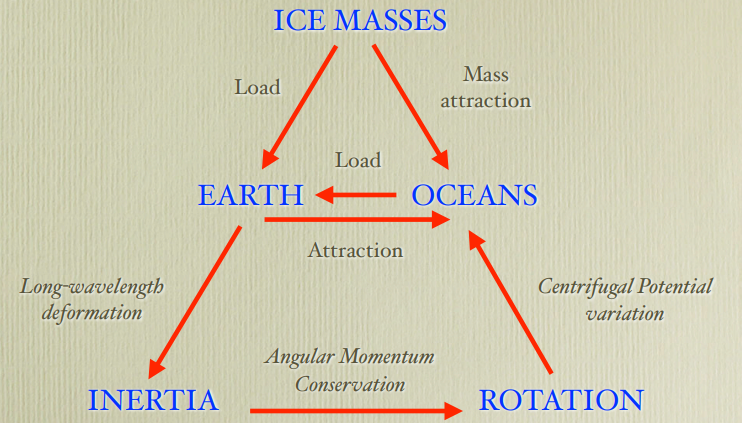
\includegraphics[width=0.7\linewidth]{fig/sea_level_variability.png}
    \caption{Interazioni fra scioglimento dei ghiacci e livello marino.}
    \label{fig:sea_level_variability}
\end{figure}

Un \textit{modello di aggiustamento isostatico} si basa sulla conoscenza della storia dei carichi di ghiacci e oceani, un modello reologico della Terra e un'equazione del livello marino.

\begin{figure}[htb]
    \centering
    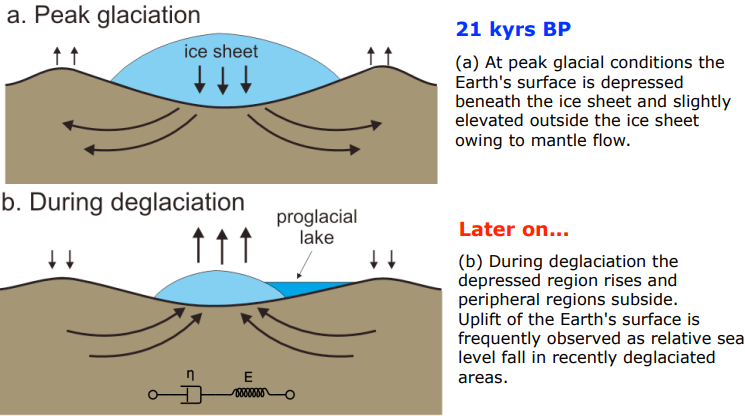
\includegraphics[width=0.7\linewidth]{fig/post-glacial_rebound.png}
    \caption{Rimbalzo post-glaciale.}
    \label{fig:post-glacial_rebound}
\end{figure}

\subsection{\textcolor{colore2}{Dinamica interna della Terra}}

Arthur Holmes fu il primo a ipotizzare, nel 1944, che all'interno del mantello terrestre l'energia fosse scambiata per convezione e che fosse possibile osservarne le conseguenze sulla superficie.\\

\noindent \textbf{Equazioni della convezione nel mantello terrestre}

\begin{itemize}
    \item Continuità (per un fluido incomprimibile): $\nabla \cdot \vec{v} = 0 $;
    \item Conservazione della quantità di moto (per un fluido Newtoniano): $- \nabla P + \eta \nabla^2 \vec{v} + \rho' \vec{g} = 0$, dove $\eta$ rappresenta la viscosità Newtoniana, $P$ la pressione e $\rho'$ la variazione nella densità del fluido;
    \item Equazione di stato: $\rho' = - \rho_0 \alpha_v (T - T_0)$, dove $\rho_0$ è la densità alla temperatura $T_0$ e $\alpha_v$ il coefficiente di dilatazione termica;
    \item Conservazione dell'energia: $\frac{\partial T}{\partial t} + (\vec{v} \cdot \nabla) T = \kappa \nabla^2 T$, dove $\kappa$ è la diffusività termica.
\end{itemize}

\noindent In un fluido stratificato in base alla temperatura, si ha convezione se la forza di galleggiamento supera quelle di attrito viscoso e di diffusione del calore.
Il rapporto fra le forze è indicato dal \textit{numero di Rayleigh}:

\begin{equation}
    Ra = \frac{Galleggiamento}{Resistenza} = \frac{\alpha \Delta T g \rho d^3}{\eta \kappa}
    \label{eq:Rayleigh}
\end{equation}

dove:
\begin{itemize}
    \item $\alpha$ rappresenta il coefficiente di espansione termica;
    \item $d$ rappresenta lo spessore del volume in cui avviene la convezione;
    \item $\eta$ rappresenta la viscosità del fluido;
    \item $\kappa$ rappresenta la diffusività termica.
\end{itemize}

\noindent Le celle convettive si formano se il numero di Rayleigh del sistema supera il valore critico di circa 2000.
All'interno del mantello si stima un valore compreso tra 20'000 e 30'000, per cui ci si aspetta che avvenga la convezione, alimentata dal gradiente termico e dal decadimento degli isotopi radioattivi.
Le celle convettive interagiscono con le placche tettoniche e la litosfera modifica i pattern delle celle convettive.\\

\noindent \textbf{Forze agenti sul moto delle placche}

Nel 1994 Uyeda iniziò a modellare le forze agenti sul sistema, considerando la subduzione dovuta allo sprofondamento delle placche, ma si hanno ancora delle domande aperte:

\begin{itemize}
    \item La convezione avviene in tutto il mantello?
    \item Sono presenti due o più strati separati in cui avviene la convezione?
    Una possibile prova del fatto che esistano almeno due strati è data dal fatto che non sono mai stati osservati sismi originati a profondità maggiori di 700 km.
    \item Prevalgono le celle convettive o i pennacchi (che attraversano il mantello in circa $10^8$ anni)?
    \item La modalità di convezione nel mantello è cambiata nel corso della storia della Terra?
    \item I moti delle placche sono consistenti con il moto del mantello?
\end{itemize}

\noindent Il flusso di calore attraverso la superficie della Terra è ovunque positivo, ma raggiunge i valori più elevati presso le dorsali oceaniche (fino a 450 $mW/m^2$).
La distribuzione dei vulcani, lungo \textit{archi vulcanici} come quello in Indonesia o in Giappone, ricalca le zone di subduzione delle placche tettoniche.

\newpage

\section{\textcolor{colore7}{Richiami sulle funzioni armoniche}}

Le funzioni armoniche permettono di studiare il campo di gravità della Terra e i fenomeni globali.

\subsection{\textcolor{colore7}{Equazione di Laplace in coordinate sferiche}}

Il \textit{Laplaciano} è un operatore differenziale del secondo ordine, definito come la divergenza del gradiente, $\nabla^2 f = \nabla \cdot (\nabla f)$, grazie al quale è possibile ricavare l'\textit{equazione di Laplace}:

\begin{equation}
    \nabla^2 f = 0
    \label{eq:Laplace}
\end{equation}

\noindent Le soluzioni dell'equazione di Laplace sono dette \textbf{funzioni armoniche}.
Un esempio è il potenziale gravitazionale all'esterno del pianeta.\\

\noindent
In coordinate sferiche, l'equazione di Laplace assume la forma:

\begin{equation}
    \frac{1}{r^2} \frac{\partial}{\partial r} \left(r^2 \frac{\partial f}{\partial r} \right) + \frac{1}{r^2 sin \theta} \frac{\partial}{\partial \theta} \left( sin \theta \frac{\partial f}{\partial \theta}\right) + \frac{1}{r^2 sin^2 \theta} \frac{\partial^2 f}{\partial \lambda^2} = 0
    \label{eq:Laplace_sf}
\end{equation}

\noindent
dove $f$ è una funzione del raggio $r$ (diretto verso l'esterno), della colatitudine $\theta$ (diretta verso sud) e della longitudine $\lambda$ (diretta verso est).
Invece di separare le variabili, si può costruire la soluzione in maniera induttiva, partendo da funzioni semplici.

\begin{figure}[!h]
    \centering
    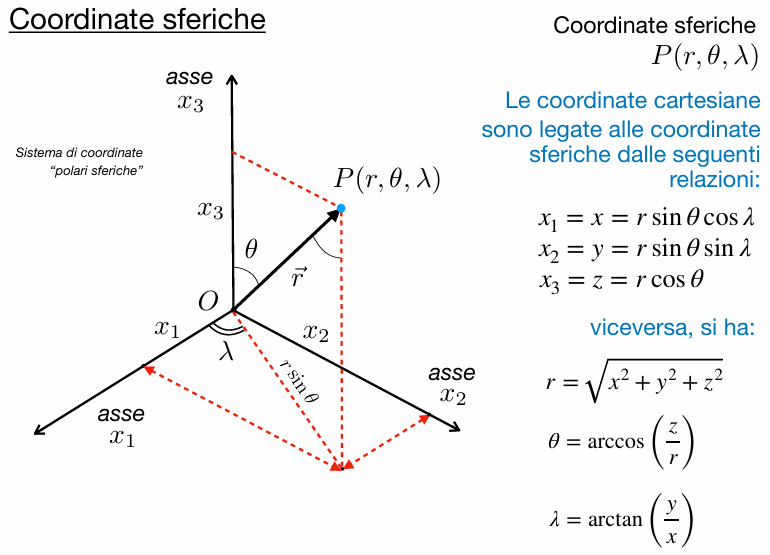
\includegraphics[width=0.6\linewidth]{fig/coordinate_sferiche.png}
    \caption{Legame tra coordinate cartesiane e sferiche.}
    \label{fig:coordinate_sferiche}
\end{figure}

\noindent
Si consideri un vettore nella forma sferica: $\boldsymbol{u} = u_r \hat{\boldsymbol{r}} + u_\theta \hat{\boldsymbol{\theta}} + u_\lambda \hat{\boldsymbol{\lambda}}$.
Le componenti cartesiane sono date da una trasformazione ortogonale.

%\begin{equation}
%    \begin{bmatrix}
%        u_x \\ u_y \\ u_z
%    \end{bmatrix} = \begin{bmatrix}
%        sin\theta cos\lambda & cos\theta cos\lambda & -sin\lambda \\ sin\theta sin\lambda & cos\theta sin\lambda & cos\lambda \\ cos\theta & -sin\theta & 0
%    \end{bmatrix} \begin{bmatrix}
%        u_r \\ u_\theta \\ u_\lambda
%    \end{bmatrix}
%    \label{eq:cartesiane_da_sferiche}
%\end{equation}

\subsection{\textcolor{colore7}{Polinomi di Legendre (LP)}}

Si tratta di \textit{polinomi ortogonali classici}, su cui si fonda la soluzione dell'equazione di Laplace in coordinate sferiche.
Sono funzioni armoniche unidimensionali e soluzioni dell'\textit{equazione di Legendre}:

\begin{equation}
    \frac{d}{dx} \left( (1 - x^2) \frac{dP_l(x)}{dx} \right) + l(l+1) P_l(x) = 0; -1 \le x \le 1 , l \in \mathbb{N}
    \label{eq:Legendre}
\end{equation}

\noindent
Per $l = 0, 1, 2, \dots$

\begin{equation}
    P_l (x) = \frac{1}{2^l l!} \frac{d^l}{dx^l} (x^2 - 1)^l
\end{equation}

\noindent Sono polinomi di grado $l$ di parità definita da $l$, che all'aumentare del grado approssimano sempre di più delle funzioni trigonometriche, mostrando una \textit{lunghezza d'onda spaziale} $\lambda_l$ data dalla \textit{regola di Jeans}:

\begin{equation}
    \lambda_l \approx \frac{2 \pi a}{l + \frac{1}{2}} \xrightarrow{l \longrightarrow \infty} \frac{2 \pi a}{l}
    \label{eq:Jeans}
\end{equation}

\noindent
\textbf{Proprietà dei Polinomi di Legendre}

\begin{enumerate}
    \item Ortogonalità: nell'intervallo $0 \le \theta \le \pi$,
    \begin{equation}
        \int_0^\pi P_l(cos\theta) P_{l'} (cos\theta) sin\theta d\theta = \frac{2 \delta_{ll'}}{2l + 1}
    \end{equation}
    cioè gli LP sono mutualmente ortogonali;
    \item Parità $P_l (1) = 1$ e $P_l (-1) = (-1)^l$;
    \item Derivate traslate: $P_l (x) = \frac{P'_{l+1}(x) - P'_{l-1}(x)}{2l+1}, l \ge 1$;
    \item Legame coi polinomi di Chebichev del secondo tipo;
    \item Funzione generatrice degli LP;
    \item Somma di Legendre: $\frac{1}{2 sin \left(\frac{\alpha}{2} \right)} \equiv \sum_{l=0}^\infty P_l (cos \alpha)$
\end{enumerate}

\noindent \textcolor{colore4}{\textbf{Distribuzione di massa sulla superficie di una sfera}}

Si consideri una concentrazione di massa, \textbf{MASCON}, come un ghiacciaio, distribuita sulla superficie della sfera secondo la legge:

\begin{equation}
    h(\theta) = \begin{cases}
        H & se \text{ } 0 \le \theta \le \alpha \\ 0 & altrimenti
    \end{cases}
\end{equation}

\noindent
Si ha cioè un disco di spessore uniforme.

\noindent
Sfruttando le proprietà dei polinomi di Legendre, si possono trovare le costanti $h_l$ tali che $h(\theta) = \sum_{l=0}^\infty h_l P_l (cos \theta)$, cioè lo \textbf{sviluppo di $h(\theta)$ in serie di polinomi di Legendre}, in cui le costanti $h_l$ sono dette \textbf{coefficienti dello sviluppo}.
Si tratta di un problema inverso.

\noindent
Il caso del cratere da impatto di Chicxulub è un esempio di applicazione di questo tipo di problemi.\\

\noindent
Integrando su tutta la sfera, si ottiene la seguente espressione analitica per i coefficienti dello sviluppo:

\begin{equation}
    h_l = \frac{2l + 1}{2} \int _0^\pi h(\theta) P_l (cos \theta) sin \theta d \theta
\end{equation}

\noindent
La soluzione analitica ha la seguente forma:

\begin{equation}
    h_l = \frac{H}{2} \begin{cases}
        1 - cos \alpha & \text{ se } l = 0 \\ P_{l-1} (cos \alpha) - P_{l+1} & \text{ se } l \ge 1
    \end{cases}
\end{equation}

\noindent Si può inoltre modificare l'espressione di $h(\theta)$ in modo che la massa della Terra sia conservata.
Questo caso può trovare un'applicazione nell'ambito dello scioglimento dei ghiacciai, che hanno una massa pari a quella che si ridistribuisce sulla superficie del pianeta.
I dischi si usano anche per rappresentare la funzione Oceano.\\

\noindent \textcolor{colore4}{\textbf{Mascon localizzato}}

Si consideri una massa puntiforme localizzata sulla superficie della sfera tramite una funzione $\delta$ di Dirac:

\begin{equation}
    h(\theta) = H \delta (1 - cos \theta) = H \sum_{l=0}^\infty h_l P_l (cos \theta) = H \sum_{l=0}^\infty \frac{2l+1}{2} P_l (cos \theta)
\end{equation}

\noindent \textcolor{colore4}{\textbf{Valore medio dei polinomi di Legendre}}

Si scopre che $P_0$ ha valore medio unitario, mentre tutti gli altri polinomi di Legendre hanno media nulla.

\begin{equation}
    \langle P_l (x) \rangle \equiv \frac{1}{2} \int _{-1} ^1 P_l (x) dx = \begin{cases}
        1 & \text{ se } l = 0 \\ 0 & \text{ altrimenti}
    \end{cases}
\end{equation}

\subsection{\textcolor{colore7}{Polinomi associati di Legendre}}

Sono soluzioni dell'equazione di Laplace che permettono di scrivere una soluzione più generale dell'equazione di Legendre.
Sono caratterizzati da un \textbf{grado} $l$ e da un \textbf{ordine} $m \le l$.
Sono polinomi se $m$ è pari.
Si costruiscono a partire dai polinomi di Legendre:

\begin{equation}
    P_{lm} (x) = (-1)^m (1 - x^2)^{m/2} \frac{d^m}{dx^m} P_l (x)
    \label{eq:polinomi_associati_legendre}
\end{equation}

\noindent
con $x = cos \theta$; il fattore $(-1)^m$ è detto \textbf{fase di Condon-Shortley} e in alcuni testi è omesso.
Polinomi associati di Legendre diversi dello stesso ordine sono mutualmente ortogonali.\\

\noindent \textcolor{colore7}{\textbf{Polinomi associati di Legendre normalizzati}}\\

\noindent
Sono spesso preferiti in geodesia e geofisica.
Si ottengono riscalando i $P_{lm}$ tramite la seguente relazione:

\begin{equation}
    \overline{P}_{lm} (x) = \sqrt{(2 - \delta _{0m}) (2l + 1) \frac{(l-m)!}{(l+m)!}} P_{lm} (x)
\end{equation}
 
\subsection{\textcolor{colore7}{Armoniche sferiche (di superficie) in forma complessa}}

Note anche come "armoniche sferiche \textit{della meccanica quantistica}", sono state utilizzate poco in geodesia per via della grande potenza di calcolo richiesta, ma permettono una trattazione agevole dei calcoli teorici.
Sono definite da:

\begin{equation}
    \mathcal{Y}_{lm} (\theta , \lambda) = \mu _{lm} P_{lm} (cos \theta) e^{im \lambda}
    \label{eq:armoniche_sferiche_complesse}
\end{equation}

\noindent
dove

\begin{equation*}
    l = 0, 1, 2, \dots \,\,\,\,\,\,\,\,\, m = -l, -l+1, \dots , l-1, l
\end{equation*}

\begin{equation*}
    \mu_{lm} \equiv \sqrt{(2l+1) \frac{(l-m)!}{(l+m)!}}
\end{equation*}

\noindent Per gli ordini negativi vale:

\begin{equation}
    \mathcal{Y}_{l-m} (\theta , \lambda) = (-1)^m \mathcal{Y}^*_{lm} (\theta , \lambda) 
\end{equation}

\noindent La scelta del coefficiente di normalizzazione $\mu_{lm}$ fa sì che l'ortonormalità sia data da:

\begin{equation}
    \int_\gamma \mathcal{Y}_{lm} (\gamma) \mathcal{Y}^*_{l'm'} (\gamma) d\gamma = 4 \pi \delta_{ll'} \delta_{mm'} 
\end{equation}

\noindent Quindi sono normalizzate a $4\pi$, mentre nel caso della meccanica quantistica, le armoniche sferiche sono normalizzate a 1.\\

\noindent Con queste definizioni, si ottengono delle funzioni armoniche \textit{solide} di forma:

\begin{equation}
    f (r, \theta , \lambda) = r^l \mathcal{Y}_{lm} (\theta, \lambda) \text{ e } f (r, \theta , \lambda) = \frac{1}{r^{l+1}} \mathcal{Y}_{lm} (\theta, \lambda)
    \label{eq:armoniche_solide}
\end{equation}

\noindent
dove la prima è regolare in $r=0$, mentre la seconda diverge.

\noindent Una soluzione generale dell'equazione di Laplace è data allora dalla combinazione lineare:

\begin{equation}
    F(r, \theta, \lambda) = \sum_{l=0}^\infty \sum_{m = -l}^l \left(a_{lm} r^l + \frac{b_{lm}}{r^{l+1}} \right) \mathcal{Y}_{lm} (\theta, \lambda)
    \label{eq:soluzione_laplace}
\end{equation}

\noindent Questa espressione costituisce lo sviluppo in armoniche sferiche di $F$.

\noindent
Definendo $(a_{lm} r^l + b/ r^{l+1}) = f_{lm}$ si ottiene invece lo sviluppo in armoniche sferiche di superficie:

\begin{equation}
    F(\theta, \lambda) = \sum_{l=0}^\infty \sum_{m = -l}^l f_{lm} \mathcal{Y}_{lm} (\theta, \lambda)
\end{equation}

\noindent
Si osserva un'importante analogia con lo spazio cartesiano: le armoniche sferiche sono la base ortonormale di uno spazio di dimensione infinita:

\begin{equation}
    \vec{v} = \sum_{i = 1}^3 v_i \hat{x}_i \longrightarrow f(\omega) = \sum_{lm} a_{lm} Y_{lm} (\omega)
\end{equation}

\noindent
Le armoniche sferiche di grado 0 sono dette \textit{termini di monopolo}, quelle di grado 1 \textit{termini di dipolo} e quelle di grado 2 \textit{termini di quadrupolo}.

Spesso si indicano le funzioni armoniche normalizzate a 1 con $Y_{lm}$ e quelle normalizzate a $4\pi$ con $\mathcal{Y}_{lm}$.

\subsection{\textcolor{colore7}{Teorema di addizione}}

Si consideri un osservatore sulla superficie della sfera, in posizione $P = (\theta, \lambda) = \gamma$, e una sorgente $S = (\theta', \lambda') = \gamma'$.
Sia $\hat{\alpha}$ l'angolo tra $S$ e $P$.

\begin{figure}[htb]
    \centering
    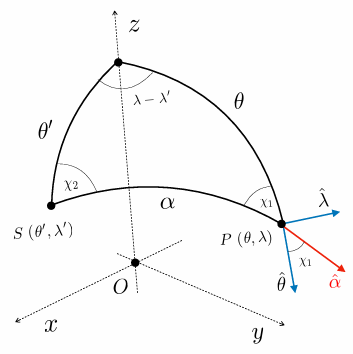
\includegraphics[width=0.45\linewidth]{fig/geometria_sferica.png}
    \caption{Geometria utile all'enunciazione dei teoremi di addizione.}
    \label{fig:geometria_sferica}
\end{figure}

\noindent Il \textbf{teorema di addizione} afferma che:

\begin{equation}
    P_l (cos \alpha) = \frac{1}{2l + 1} \sum_{m=-l}^l \mathcal{Y}^*_{lm} (\gamma') \mathcal{Y}_{lm} (\gamma)
    \label{eq:addizione}
\end{equation}

\noindent
Formule analoghe valgono anche per i gradienti.

\subsection{\textcolor{colore7}{Armoniche sferiche in forma reale}}

Sono una forma reale delle funzioni armoniche di superficie, che formano un sistema ortonormale completo di funzioni, di ampio utilizzo nelle applicazioni pratiche.
La forma generica è:

\begin{equation}
    R_{lm} (\theta, \lambda) = (c_{lm} cos m \lambda + s_{lm} sin m \lambda ) P_{lm} (cos \theta)
\end{equation}

\noindent
con $c_{lm}$ e $s_{lm}$ coefficienti reali adimensionali e $P_{lm}$ polinomi di Legendre non normalizzati.\\

\noindent
Si hanno tre tipi di armoniche sferiche (Figura \ref{fig:spherical_harmonics}):

\begin{itemize}
    \item Zonali $(m=0)$, che si annullano su $l$ paralleli;
    \item Tesserali $(0 < m < l)$, che si annullano su $l-m$ paralleli e $2m$ meridiani;
    \item Settoriali $(m=l)$, che si annullano su $2m$ meridiani.
\end{itemize}

\begin{figure}[h]
    \centering
    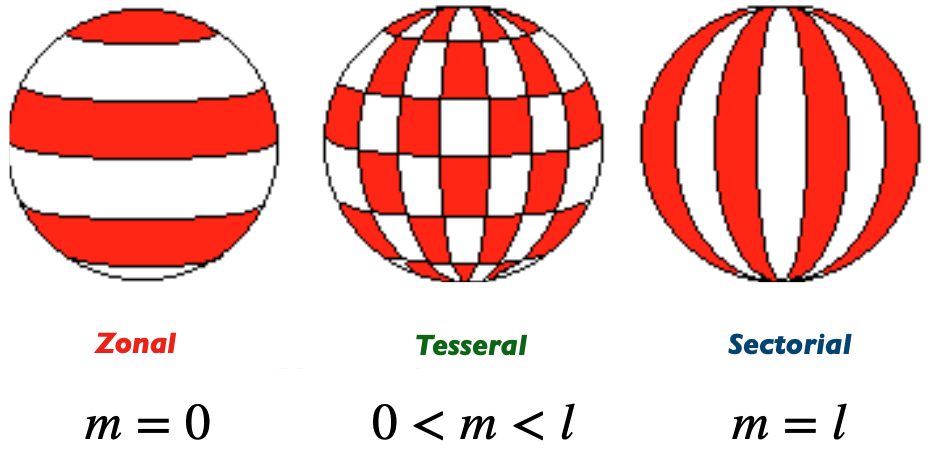
\includegraphics[width=0.7\linewidth]{fig/spherical_harmonics.png}
    \caption{Tre tipi di armoniche sferiche.}
    \label{fig:spherical_harmonics}
\end{figure}

\noindent Le armoniche sferiche di grado 2 hanno un ruolo fondamentale nella descrizione delle maree.

\subsection{\textcolor{colore7}{Sviluppo in serie di armoniche sferiche}}

Le armoniche sferiche permettono di rappresentare ogni funzione che varia sulla superficie di una sfera tramite una combinazione lineare, in maniera analoga a come le serie di Fourier permettono di fare con le funzioni che variano nel tempo.

\noindent
Sia $f(\gamma)$ una funzione reale e a quadrato sommabile, con $\gamma = (\theta, \lambda)$. Si consideri la formula diretta:

\begin{equation}
    f(\gamma) = \sum _{lm} f_{lm} \mathcal{Y}_{lm} (\gamma)
\end{equation}

\noindent
Si moltiplica per $\mathcal{Y}^*_{l'm'}(\gamma)$:

\begin{equation}
    f(\gamma) \mathcal{Y}^*_{l'm'}(\gamma) = \sum _{lm} f_{lm} \mathcal{Y}_{lm} (\gamma) \mathcal{Y}^*_{l'm'}(\gamma)
\end{equation}

\noindent
Si integra sulla superficie della sfera:

\begin{equation}
    \int_\gamma f(\gamma) \mathcal{Y}^*_{l'm'}(\gamma) d \gamma = \sum _{lm} f_{lm} \int _\gamma \mathcal{Y}_{lm} (\gamma) \mathcal{Y}^*_{l'm'}(\gamma) d \gamma
\end{equation}

\noindent
Si sfrutta la normalizzazione:

\begin{equation}
     \int_\gamma f(\gamma) \mathcal{Y}^*_{l'm'}(\gamma) d \gamma = 4 \pi \sum _{lm} f_{lm} \delta_{ll'} \delta_{mm'} = 4 \pi f_{l'm'}
\end{equation}

\noindent
Si ricava così la formula inversa:

\begin{equation}
    f_{lm} = \frac{1}{4\pi} \int_\gamma f(\gamma) \mathcal{Y}^*_{lm} (\gamma) d\gamma
\end{equation}

\noindent
Il problema inverso costituito dal calcolo dei coefficienti $f_{lm}$ richiede di conoscere la funzione $f(\gamma)$ su tutta la superficie della sfera, il che risulta spesso impossibile in campo geofisico. 
Questo limita il calcolo di $f_{lm}$ e il valore di $l_{max}$ a un valore finito, che dipende dalla densità dei punti di griglia.\\

\noindent
Lo sviluppo complesso è equivalente a quello reale:

\begin{equation}
    f(\gamma) = \sum_{l=0}^\infty \sum_{m=-l}^l f_{lm} \mathcal{Y}_{lm}(\gamma)
\end{equation}

\noindent
In geodesia, gli sviluppi reali normalizzati sono convenzionalmente usati per la descrizione del potenziale del campo di gravità.

\subsection{\textcolor{colore7}{Statistica sulla sfera}}

Le oscillazioni spaziali delle armoniche sferiche non sono equispaziate, ma hanno una lunghezza caratteristica che si può stimare grazie alla \textit{Regola di Jeans} (vedi \ref{eq:Jeans}), dove $2\pi a \approx 40'000 km$.\\

\noindent
Possiamo caratterizzare l'andamento di una data funzione $f(\gamma)$ sulla sfera usando definizioni statistiche elementari.
La media di $f(\gamma)$ sulla sfera unitaria è:

\begin{equation}
    \langle f (\gamma) \rangle \equiv \frac{1}{4 \pi} \int _\gamma f(\gamma) d\gamma
\end{equation}

\noindent 
con $d \gamma = sin \theta d \theta d \lambda $ l’elemento di area sulla superficie della sfera unitaria.\\
La formula deriva dalle proprietà dei polinomi di Legendre, per cui è possibile valutare immediatamente la media:

\begin{equation}
    \langle \mathcal{Y}_{lm} (\gamma) \rangle = \frac{1}{4 \pi} \int_\gamma \mathcal{Y}_{lm} (\gamma) d \gamma = \frac{1}{4 \pi} \int _\gamma \mathcal{Y}_{lm} (\gamma) \mathcal{Y}^*_{00} (\gamma) d \gamma = \delta _{l0} \delta _{m0}
\end{equation}

\noindent La media si può relazionare ai coefficienti dello svilupo:

\begin{align}
    \langle f (\gamma) \rangle &= \frac{1}{4 \pi} \int_\gamma f(\gamma)d\gamma = \frac{1}{4 \pi} \int_\gamma \left( \sum_{lm} f_{lm} \mathcal{Y}_{lm} (\gamma) \right)d\gamma \\ &= \frac{1}{4 \pi} \sum_{lm} f_{lm} \int_\gamma \mathcal{Y}_{lm} (\gamma) d\gamma = \sum_{lm} f_{lm} \langle \mathcal{Y}_{lm} \rangle = \sum_{lm} f_{lm} \delta_{l0} \delta_{m0} \\ &= f_{00} 
\end{align}

\noindent
Quindi solo l'armonica di grado e ordine $(l,m) = (0,0)$, ovvero $\mathcal{Y}_{00} = 1$ ha media unitaria, tutte le altre hanno media nulla.
Se $f(\gamma)$ ha media nulla sulla superficie unitaria $\gamma$, allora nel suo sviluppo manca il termine $(l,m) = (0,0)$.\\

\noindent
La varianza di una funzione $f(\gamma)$ sulla sfera unitaria è:

\begin{equation}
    var(f) \equiv \sigma^2 (f) = \langle f^2 \rangle - \langle f \rangle^2
\end{equation}

\noindent La \textit{potenza totale} di una funzione reale $f(\gamma)$ è:

\begin{equation}
    TP = \frac{1}{4 \pi} \int_\gamma f^2 (\gamma) d \gamma \equiv \langle f^2(\gamma) \rangle
\end{equation}

\noindent
La potenza totale coincide, per funzioni a media nulla, con la varianza $\sigma^2$.
Sviluppando il calcolo si ottiene:

\begin{align}
    TP &= \frac{1}{4 \pi} \int_\gamma f(\gamma)f^*(\gamma)d\gamma = \frac{1}{4 \pi} \int_\gamma \left( \sum_{lm} f_{lm} \mathcal{Y}_{lm} (\gamma) \right) \left( \sum_{l'm'} f^*_{l'm'} \mathcal{Y}^*_{l'm'} (\gamma) \right)d\gamma \\ &= \frac{1}{4 \pi} \sum_{lm}  \sum_{l'm'}f_{lm} f^*_{l'm'} \int_\gamma \mathcal{Y}_{lm} (\gamma) \mathcal{Y}^*_{l'm'} (\gamma) d\gamma = \frac{1}{4 \pi} \sum_{lm}  \sum_{l'm'}f_{lm} f^*_{l'm'} \delta_{ll'} \delta_{mm'} = \sum_{lm} f_{lm} f^*_{lm} \\ &= \sum_{l=0}^\infty S_{ff}(l)
\end{align}

\noindent
dove si usa la definizione di \textit{spettro armonico}:

\begin{equation}
    S_{ff} (l) = \sum _{m = - l}^lf_{lm} f^*_{lm}
\end{equation}

\noindent Si definisce anche la \textit{densità spettrale} di $f(\gamma)$:

\begin{equation}
    SD = \frac{1}{2l+1} S_{ff}(l)
\end{equation}

\noindent La \textit{potenza incrociata} di due funzioni reali $f(\gamma)$ e $g(\gamma)$ è:

\begin{equation}
    CP = \frac{1}{4 \pi} \int_\gamma f(\gamma) g^*(\gamma) d\gamma = \sum_{l=0}^\infty S_{fg}(l)
\end{equation}

\noindent
dove si indica lo \textit{spettro di potenza incrociato} delle due funzioni:

\begin{equation}
    S_{fg} (l) = \sum_{m=-l}^l f_{lm}g^*_{lm}
\end{equation}

\noindent Grazie alla \textit{correlazione grado per grado} fra due funzioni reali $f(\gamma)$ e $g(\gamma)$ è possibile stabilire quanto i due campi siano correlati fra loro e su quale scala spaziale:

\begin{equation}
    C_{fg} (l) = \frac{S_{fg} (l)}{\sqrt{S_{ff}(l)} \sqrt{S_{gg}(l)}} \text{ , con } -1 \le C(l) \le 1
\end{equation}

\noindent
Se $f = g$ si ha $C_{fg}(l) = 1$, mentre se $f = -g$ si ha $C_{fg}(l) = -1$.\\

\noindent
Le ondulazioni del geoide fanno sì che la correlazione fra i campi di geoide e topografia (Figura \ref{fig:correlation}) sia molto alta per valori di $l \ge 15$: il geoide a piccola scala riflette la topografia, per via di fenomeni come l'isostasia, mentre a grande scala la correlazione è inferiore perché il geoide risponde alle anomalie di densità associate alla dinamica interna della Terra.\\

\noindent
Si usa inoltre l'\textit{indice di correlazione lineare di Pearson} $\rho$ per esprimere un'eventuale relazione di linearità fra due variabili statistiche.

\subsection{\textcolor{colore7}{Spettro armonico}}

Lo \textit{spettro armonico} o \textit{power spectral density} permette di determinare quanta energia vi sia in ciascuna oscillazione armonica che compone una funzione.
Data una funzione:

\begin{equation}
    f(\gamma) = \sum _{l=o}^{l_{max}} \sum_{m=-l}^l f_{lm} \mathcal{Y}_{lm}(\gamma)
\end{equation}

\noindent Si definisce lo spettro come:

\begin{equation}
    PSD(l) = \frac{1}{2l+1} \sum_{m=-l}^l f_{lm} f^*_{lm}
\end{equation}

\noindent In molti casi lo spettro armonico varia con il grado armonico seguendo una legge di potenza:

\begin{equation}
    S^2_l(f) = Al^\beta
\end{equation}

\noindent
Per cui si distinguono tre casi:

\begin{itemize}
    \item $\beta = 0$: tutti i gradi armonici hanno la stessa energia e lo spettro è detto \textit{bianco};
    \item $\beta < 0$: l'energia decade con il grado armonico e lo spettro è detto \textit{rosso};
    \item $\beta > 0$: l'energia cresce con il grado armonico e lo spettro è detto \textit{blu}.
\end{itemize}

\noindent
In particolare, lo spettro del geoide segue la \textit{regola di Kaula}: $S \propto l^{-2.16}$, ma il significato di questa osservazione non è ancora stato compreso.\\

\noindent \textbf{\textcolor{colore4}{Spettro armonico della $\delta$ di Dirac}}\\

\noindent
Sviluppando la $\delta$ di Dirac in funzioni armoniche e applicando il teorema di addizione, si osserva che lo spettro non dipende dal grado, per cui è bianco. 

\subsection{\textcolor{colore4}{Funzione Oceano}}

Un'importante applicazione delle funzioni armoniche è quella dell'analisi spettrale di un campo scalare come quello della \textit{funzione Oceano}, definita come:

\begin{equation}
    O (\gamma) = \begin{cases}
        1 & \text{ se $\gamma$ è nel mare} \\ 0 & \text{ se $\gamma$ è sulla terraferma}
    \end{cases}
    \label{eq:funzione_oceano}
\end{equation}

\begin{figure}[h!]
    \centering
    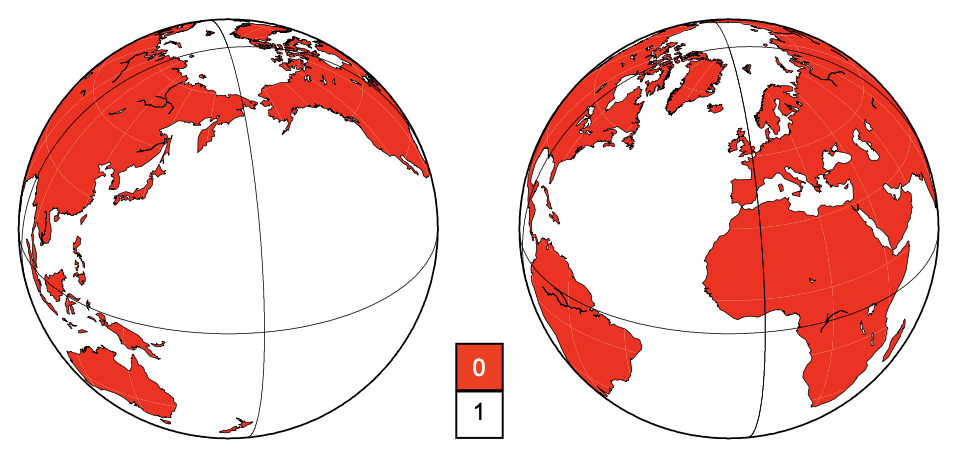
\includegraphics[width=0.6\linewidth]{fig/funzione_oceano.png}
    \caption{Funzione Oceano}
\end{figure}

\noindent Tale funzione dipende dal tempo e dal livello del mare, per cui ci si focalizza su un istante fissato e si decompone in funzioni armoniche:

\begin{equation}
    O (\gamma) = \sum_{lm}^{l_{max}} o_{lm} \mathcal{Y}_{lm} (\gamma)
\end{equation}

\noindent Risolvere il problema inverso significa determinare i coefficienti:

\begin{equation}
    o_{lm} = \frac{1}{4\pi} \int_\gamma O (\gamma) \mathcal{Y}^*_{lm} (\gamma) d\gamma \equiv \frac{1}{4\pi} \int_{oceano} \mathcal{Y}^*_{lm} (\gamma) d\gamma
\end{equation}

\noindent Tale integrale si può valutare solo numericamente, attraverso due approcci:\\

\noindent \textbf{A: metodo classico}\\

\noindent
Si suddivide la superficie terrestre in $N$ quadrilateri, così da spezzare il calcolo di $o_{lm}$ nella somma di $N$ contributi.
Si verifica che lo spettro della funzione Oceano è rosso e che gli oceani hanno un peso maggiore rispetto ai dettagli più piccoli.

\noindent In particolare il coefficiente $o_{00}$ vale 0.71, che riflette la frazione della superficie terrestre ricoperta da oceani.

\noindent Grazie ai coefficienti armonici dello sviluppo è possibile ricostruire la funzione originale grazie alla combinazione lineare delle armoniche sferiche complesse.
Si nota che ponendo $l_{max} = 72$ si ottengono delle linee di costa squadrate che riflettono la suddivisione operata in questo approccio.\\

\noindent \textbf{B: metodo geodetico}\\

\noindent
Si suddivide la superficie terrestre in una griglia geodesica in cui ogni cella ha area equivalente, con la geometria basata su quella dell'icosaedro.
L'idea, già utilizzata in ambito astrofisico per la CMB, fu applicata inizialmente da Max Tegmark.\\

\noindent
Il numero di pixel $N_p$ dipende dalla risoluzione $R$ secondo la legge:

\begin{equation}
    N_p = 40R(R-1)+12
\end{equation}

\noindent Il vantaggio di questo metodo sta nel fatto che l'area delle celle è equivalente, il che rende il calcolo molto più agevole.
Un metodo simile si basa sulla griglia di Fibonacci regolarizzata ai poli.

\newpage

\section{\textcolor{colore2}{Geosfera, geodinamica e Sistema Terra}}

All'inizio del XX secolo, il pioniere della ricerca polare Alfred Wegener propose la \textbf{teoria della deriva dei continenti}, su cui si basa l'odierna \textbf{teoria della tettonica delle placche} (dal greco "costruire").
La teoria, secondo la quale le masse continentali si muovono lentamente separandosi da un unico supercontinente chiamato Pangea, fu inizialmente screditata.
Solamente a partire dagli anni Cinquanta fu accettata, grazie a nuove scoperte a supporto di questa teoria, come evidenze nel campo del paleomagnetismo.\\

\noindent
La tettonica, o geologia strutturale, studia gli spostamenti e le deformazioni della crosta terrestre.
Si ipotizza che la crosta possa sprofondare fino al mantello e interagire con le inversioni del campo magnetico.
La convezione del mantello è compatibile con le ondulazioni osservate del geoide (di circa 10 m).

\subsection{\textcolor{colore2}{Deriva dei continenti}}

Wegener non conosceva i fondali oceanici, così basò la sua teoria su una serie di osservazioni condotte sulle superfici dei continenti:

\begin{itemize}
\item Evidenze paleontologiche: alcuni fossili di organismi simili si trovano a grande distanza, come il caso del mesosauro, ritrovato in Africa ed in Sud America;
\item Evidenze paleoclimatiche: alcune antiche glaciazioni (come quella del Permiano, 300-250 milioni di anni fa) hanno lasciato delle tracce in continenti adesso separati dagli oceani, come Sud America, Africa, India, Australia e Antartide.
%non ci sono anche quelle geologiche?
%non ho visto niente nelle slide e nemmeno nei miei appunti
\end{itemize}

\noindent
In precedenza, osservando il profilo delle coste atlantiche di Sud America e Africa, Antonio Snider-Pellegrini (1802-1885) teorizzò la possibilità della deriva dei continenti causata dal diluvio universale e Seuss teorizzò che le catene montuose si fossero formate per la contrazione del pianeta, dovuta al suo raffreddamento.

Attualmente si teorizza che circa 250 milioni di anni fa i continenti attuali fossero riuniti in un'unica massa continentale, detta \textit{Pangea}.
Probabilmente in precedenza si verificarono altri eventi simili.\\

\noindent
\textbf{Problemi della teoria della deriva dei continenti}

\begin{enumerate}
    \item Per la sismologia la Terra è un corpo solido, in cui si propagano le onde elastiche, mentre per la deriva dei continenti questi si muovono su un fluido;
    \item Non è chiaro quale forza origini la deriva dei continenti.
\end{enumerate}

\noindent
Wegener propose una forza detta \textit{Polflucht} (dal tedesco "volo dai poli"), dovuta alla forza centrifuga, che sposterebbe i continenti verso l'Equatore, ma essa sarebbe comunque troppo debole per spiegare questa disgregazione.

\subsection{\textcolor{colore2}{Osservazioni a supporto della teoria della tettonica delle placche}}

\begin{itemize}
    \item Forma dei fondali oceanici: le osservazioni sono iniziate nella seconda metà del XX secolo, ma l'esistenza di una dorsale medioatlantica fu proposta già a durante il XIX secolo da Matthew Fontaine Maury.
    Il sistema di rilievi sottomarini si estende per circa 50'000 km in tutto il mondo e raggiunge un'altezza media di circa 4500 m rispetto al fondale circostante.
    Lo spessore dei sedimenti sui fondali è inoltre decisamente inferiore a quanto ci si potrebbe aspettare considerando un deposito durato centinaia di milioni di anni;
    \item Esistenza delle anomalie magnetiche: le inversioni del campo magnetico terrestre non seguono una legge chiara (183 inversioni negli ultimi 83 milioni di anni, l'ultima avvenuta 780 mila anni fa).
    Anche la durata di tali inversioni è variabile: si stima che durino tra i 2 e i 12 mila anni.
    Glatzmaier e Roberts modellarono per primi l'inversione.\\

    \begin{figure}[h!]
        \centering
        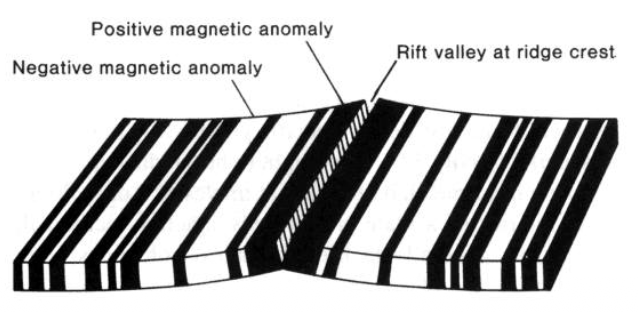
\includegraphics[width=0.5\linewidth]{fig/magnetic_anomalies.png}
        \caption{Anomalie magnetiche dei fondali oceanici.}
    \end{figure}

    Le indagini magnetometriche evidenziano la simmetria delle anomalie magnetiche attorno all'asse delle creste oceaniche.
    È possibile determinare l'orientamento del campo magnetico terrestre mediante la magnetizzazione residua acquisita dai minerali ferromagnetici quando, raffreddandosi al di sotto della temepratura di Curie, si magnetizzano parallelamente al campo magnetico pesente in quel momento;
    \item Ipotesi dell'allargamento dei fondali marini: come può aggiungersi nuova crosta lungo le creste oceaniche senza che la dimensione o la massa della Terra aumentino?
    Harry Hess trovò una spiegazione ipotizzando che la crosta oceanica ridiscenda nel mantello nei pressi delle fosse oceaniche, così che i fondali vengano "riciclati" velocemente, in accordo con l'età media della crosta oceanica, di circa 150 milioni di anni.
    Questo spiega perché le rocce oceaniche sono più giovani di quelle continentali;

    \begin{figure}[h!]
        \centering
        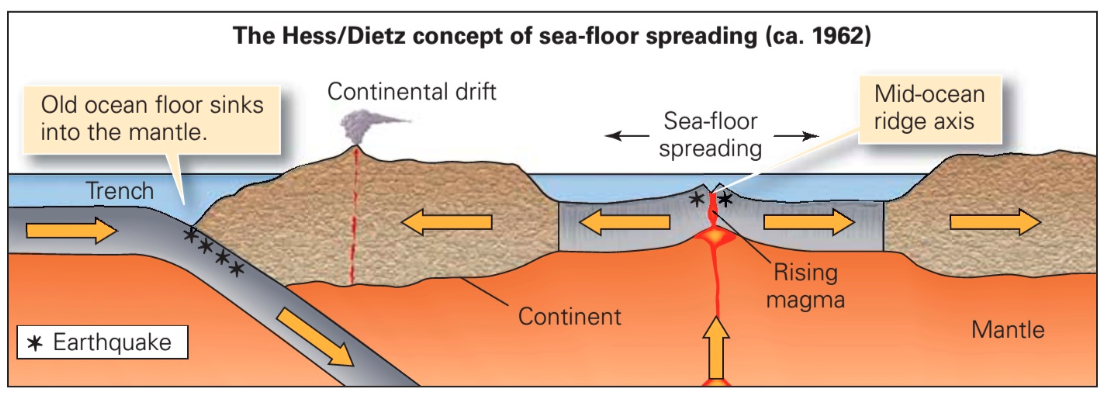
\includegraphics[width=0.6\linewidth]{fig/seafloor_spreading.png}
        \caption{Seafloor spreading.}
    \end{figure}

    \item Raffreddamento della litosfera oceanica: il flusso di calore attraverso la superficie è massimo nei pressi delle dorsali oceaniche, in accordo con la minore età della litosfera in queste zone.
    Le misure sono condotte grazie a delle sonde che sfruttano la legge della conduzione di calore di Fourier:

    \begin{equation}
        q_s \approx -k \frac{dT}{dy}
    \end{equation}

    \begin{figure}[h!]
        \centering
        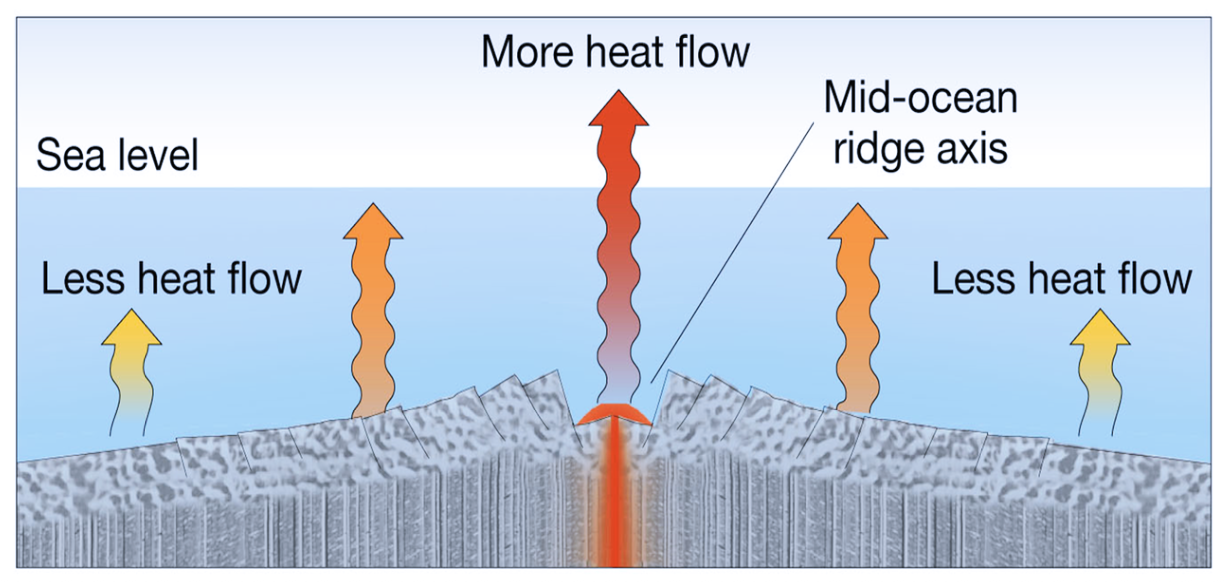
\includegraphics[width=0.5\linewidth]{fig/heat_flow.png}
        \caption{Flusso di calore attraverso la litosfera.}
    \end{figure}

    Il flusso di calore decresce con l'età del fondale, secondo la legge $q_s \propto \frac{1}{\sqrt{\text{età}}}$, che funziona molto bene con i dati disponibili.
    Questa legge tende però a sovrastimare il flusso di calore per la litosfera più recente e sovrastimarlo per quella più antica; c'è invece maggiore accordo per la litosfera di età compresa tra 50 e 100 milioni di anni.\\
    
    \noindent
    Per il principio di isostasia la profondità dell'oceano aumenta per compensare la contrazione termica della litosfera, da cui la legge Batimetria = $A + B\sqrt{\text{età}}$.
    In generale quando la risalita del materiale a causa dell'apertura dei fondali è più veloce, il livello marino è maggiore, mentre quando il processo è più lento il livello marino è minore, per via della conservazione del volume oceanico;

    \begin{figure}[htb]
        \centering
        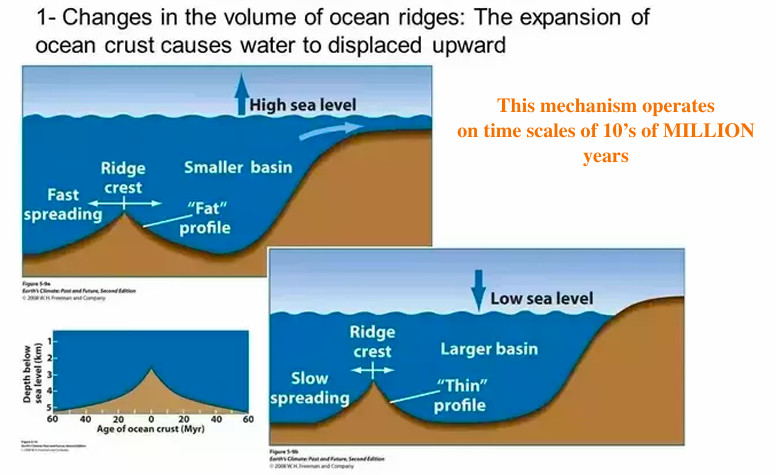
\includegraphics[width=0.5\linewidth]{fig/seafloor_shape.png}
        \caption{Cause tettoniche dei cambiamenti del livello marino.}
        \label{fig:seafloor_shape}
    \end{figure}

    \item Terremoti e vulcani: i terremoti tendono a concentrarsi lungo le linee di faglia interessate dalla tettonica delle placche, in particolare presso le dorsali oceaniche (a profondità minime) e le fosse oceaniche.
    In queste ultime, i terremoti seguono le zone di Wadati-Benioff, superfici inclinate di 40-60$^\circ$ che raggiungono i 700 km di profondità.
    Al contrario, nei pressi delle creste oceaniche si osservano terremoti a profondità minime.
    Il riconoscimento di tale connessione conferma l'ipotesi di allargamento del fondale marino: questo processo interessa le zone in cui la crosta oceanica viene generata (lungo le creste) e le zone in cui la litosfera affonda nel mantello (fosse oceaniche).
    
    Il vulcanismo si manifesta prevalentemente lungo i confini delle placche litosferiche:
    per il 75\% come vulcanismo sottomarino presso le dorsali, in corrispondenza dei punti in cui le placche si allontanono
    e in parte come vulcanismo subaereo nelle zone di subduzione e in punti interessati da pennacchi di risalita dal mantello, come le isole del Pacifico.
    Esistono inoltre dei punti caldi (\textit{hotspots)}, come quelli delle Hawaii o di Yellowstone, alimentati dal mantello sottostante, che presenta una temperatura più elevata rispetto a quella del mantello circostante.
    La posizione di questi \textit{hotspots} sulla superficie della Terra è indipendente dal movimento delle placche, per cui possono creare delle catene di vulcani che si muovono sopra di esse;

    \item Placche tettoniche: esistono circa 15 placche maggiori, separate fra loro da 3 diversi tipi di margini (divergenti, convergenti e trascorrenti o trasformi).
    Il moto di ogni placca è una rotazione rigida attorno ad un asse detto \textit{asse di Eulero}, grazie al quale si può  caratterizzare il campo di velocità delle placche e di conseguenza i tipi di margini.
    Nota la velocità delle placche, è possibile valutarne la divergenza (che indica creste e fosse oceaniche) e il rotore (da cui la vorticità e la caratterizzazione dei margini trascorrenti).

    \begin{figure}[!h]
        \centering
        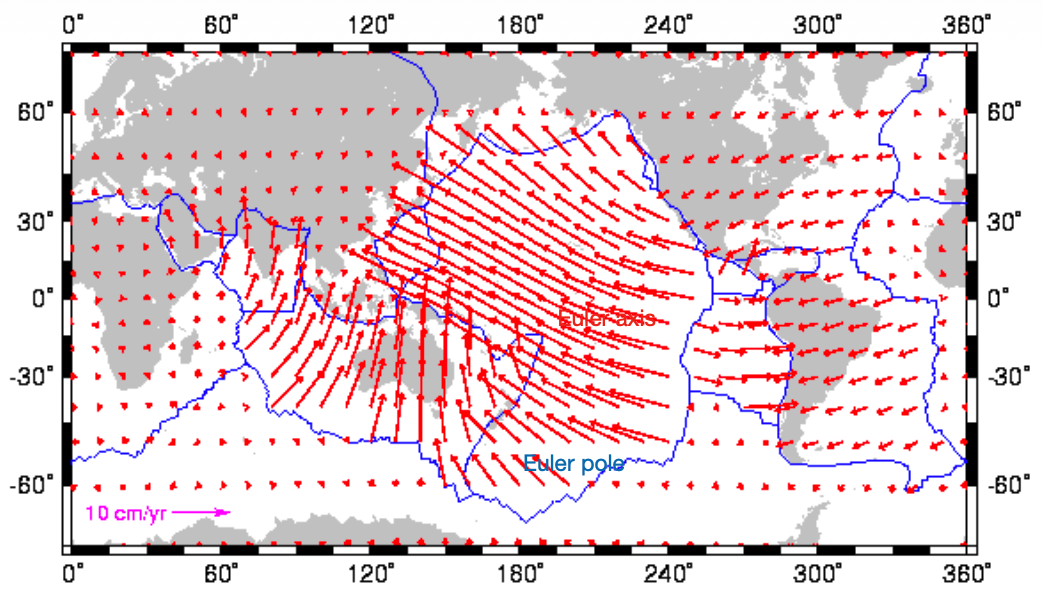
\includegraphics[width=0.65\linewidth]{fig/tettonica_placche.png}
        \caption{Campo di velocità delle placche tettoniche.}
    \end{figure}

    Il movimento complessivo delle placche, che si può tracciare rispetto al sistema di riferimento dei punti caldi, è diretto verso ovest (\textit{westward drift della litosfera}): si ha cioè una rotazione netta delle placche.
    La placca Pacifica, priva di massa continentale, ha vorticità trascurabile e risulta la più veloce ed energetica.
    Un controesempio è fornito da Marte, su cui si osservano gli effetti del vulcanismo antico, ma non dello spostamento delle placche sulla superficie.
    Su Venere invece la convezione è molto più lenta e ostacolata per via della minore presenza di acqua nel mantello.
    L'attività tettonica è studiata anche sui satelliti di Giove.
\end{itemize}

\newpage

\section{\textcolor{colore7}{Campo di Gravità}}

\subsection{\textcolor{colore2}{Distribuzioni di massa}}

Lo studio di come la massa è distribuita all'interno di un corpo è fondamentale per comprenderne il comportamento dinamico.
Nel caso del nostro pianeta, il campo di gravità e la forma stessa della Terra sono la manifestazione diretta della sua distribuzione interna di massa.
Di conseguenza, analizzare queste distribuzioni risulta essenziale per la geodesia e la geofisica.\\

\noindent
Le componenti fluide della Terra e il suo moto di rotazione ne influenzano il campo di gravità.
Per un corpo deformabile come la Terra, infatti, la distribuzione della massa è fortemente influenzata dalla rotazione stessa; viceversa, qualsiasi variazione temporale nella distribuzione delle masse va a modificare i parametri di rotazione terrestre.


Le distribuzioni di massa variano nel tempo a causa di una vasta gamma di processi che spaziano su diverse scale temporali:
processi climatici come variazioni a breve e lungo termine legati al ciclo dell'acqua, allo scioglimento dei ghiacci e alle dinamiche atmosferiche e oceaniche;
processi geologici, quindi dinamiche interne profonde che operano su scale temporali molto più lunghe.

Le ondulazioni del geoide sono influenzate maggiormente da questi ultimi processi, che dipendono dalla distribuzione di massa a grande profondità.\\

\noindent
Secondo il \textbf{modello PREM} è possibile descrivere la Terra grazie ad una serie di sfere concentriche caratterizzate da proprietà diverse, mentre nella realtà questa simmetria viene meno, a cause di asimmetrie nelle distribuzioni di massa e dipendenze temporali.
Le variazioni del campo di gravità sono attualmente misurate dai satelliti GRACE.
Le proprietà reologiche (che regolano la velocità delle onde sismiche) e la densità (da cui dipende il campo di gravità) dipendono solo dalla distanza dal centro.

\subsection{\textcolor{colore7}{Momenti delle distribuzioni}}

Un continuo è un altro modello molto utilizzato per studiare le distribuzioni di massa senza particolari assunzioni di simmetria.
Essa è caratterizzata da alcuni momenti, tra cui:

\begin{itemize}
    \item Massa (momento di ordine 0). È uno scalare (tensore di rango 0) che dipende solo dalla densità locale:

    \begin{equation}
        M \equiv \int_V \rho (\vec{x}) dV
    \end{equation}

    \noindent
    dove la densità $\rho$ è definita come $\rho(\vec{x}) = dm/dV$.
    La densità media è quindi: $\bar{\rho} = M/V$.
    
    \item Centro di massa (momento di ordine 1). È un vettore (tensore di rango 1) dato da:

    \begin{equation}
        \vec{x}_{CM} \equiv \frac{\int_V \vec{x}dm}{\int_V dm} = \frac{1}{M} \int_V \vec{x} dm
    \end{equation}

    \noindent rappresenta la media del vettore poszione $\vec{x}$ pesata sulla distribuzione di massa.\\

    \noindent
    Le sue componenti sono:

    \begin{equation}
        (x_1, x_2, x_3)_{CM} = \frac{1}{M} \left(\int_V x_1 dm , \int_V x_2 dm , \int_V x_3 dm\right)
    \end{equation}

    È sempre possibile scegliere un sistema di riferimento in cui il centro di massa si annulla: è il sistema in cui l'origine coincide con il centro di massa.

    \item Momento di inerzia (momento di ordine 2). È un tensore (di rango 2) simmetrico a valori reali con 6 componenti indipendenti.
    
    \begin{equation}
        I_{ij} = \int_V (x_lx_l \delta_{ij} - x_ix_j)dm = \begin{pmatrix}
            I_{11} & I_{12} & I_{13} \\ I_{21} & I_{22} & I_{23} \\ I_{31} & I_{32} & I_{33}
        \end{pmatrix}
        \label{eq:inerzia}
    \end{equation}

    I tre \textit{elementi diagonali} sono dati da:
    
    \begin{equation}
        I_{ii} = \int_V (x_j^2 + x_k^2) dm
    \end{equation}
    
    mentre i \textit{prodotti di inerzia} sono dati da:
    
    \begin{equation}
        I_{ij} = I_{ji} = - \int_V x_ix_j dm
    \end{equation}

    \textbf{Proprietà del momento di inerzia}:

    Gli autovettori di $I_{ij}$ (\textit{assi principali}) sono ortogonali fra loro e formano una base;

    Gli autovalori di $I_{ij}$ sono reali e vale $I_1 < I_2 < I_3$;

    La traccia $Tr(I_{ij})$ è invariante a seguito di un cambio di sistema di riferimento;

    Il determinante è invariante a seguito di un cambio di sistema di riferimento.

    \end{itemize}

\subsection{\textcolor{colore7}{Legge della gravitazione di Newton}}

Dalla legge della gravitazione di Newton segue che il moto di due corpi puntiformi che interagiscono tramite questa legge è descritto dalle \textbf{leggi di Keplero}:

\begin{enumerate}
    \item L'orbita di un pianeta è un'ellisse e il Sole è in uno dei due fuochi.
    \item La congiungente copre aree uguali in tempi uguali.
    \item Il rapporto tra il quadrato del periodo di rivoluzione e il cubo del semiasse maggiore dell'orbita è costante:

    \begin{equation}
        \frac{T^2}{R^3} = K
    \end{equation}
    
\end{enumerate}

\noindent
Nel caso di corpi più complessi, come la Terra, le irregolarità misurate da appositi satelliti permettono di ottenere informazioni sul campo di gravità.\\

\noindent Si definisce il \textit{campo gravitazionale} in un punto P:

\begin{equation}
    \vec{g}(P) \equiv \frac{\vec{F}}{m} = \frac{GM}{r^2} \hat{r}
\end{equation}

\noindent
Quindi, per una distribuzione di massa si sfrutta il principio di sovrapposizione:

\begin{equation}
    \vec{g}(P) = G \sum_{n} \frac{m_n}{r_n^2} \hat{r}_n
    \label{eq:campo_gravitazionale}
\end{equation}

\noindent
Siccome si tratta di un campo centrale, la circuitazione è nulla e, grazie al teorema di Stokes, si dimostra che è anche irrotazionale.
Si può allora definire il campo a partire da un \textbf{potenziale gravitazionale} scalare: $\vec{g} = \nabla U$.\\

\noindent
Il flusso del campo gravitazionale attraverso una superficie sferica $S$ di raggio $r$ è dato da:

\begin{equation}
    \Phi_S (\vec{g}) \equiv \int_S \vec{g} \cdot \vec{S} = \int_S \vec{g} \cdot \hat{n} dS = 4 \pi r^2 \vec{g} \cdot \hat{n} = - 4 \pi r^2 \frac{GM}{r^2} = - 4 \pi GM
\end{equation}

\noindent
cioè dipende solamente dalla massa contenuta nella sfera (legge di Gauss per il campo gravitazionale).\\

\noindent
Usando la definizione di densità e il teorema della divergenza:

\begin{equation}
    \Phi_S (\vec{g}) = -4 \pi G M_{in} = -4 \pi G \int_V \rho (\vec{x}) dV = \int_V \nabla \cdot \vec{g} dV
\end{equation}

\noindent
Quindi la divergenza di $\vec{g}$ è:

\begin{equation}
    \nabla \cdot \vec{g} = - 4 \pi G \rho (\vec{x})
\end{equation}

\noindent
Dato che $\vec{g} = \nabla U$, otteniamo che il potenziale gravitazionale $U$ soddisfa l'equazione di Poisson all'interno e l'equazione di Laplace all'esterno del pianeta, per cui è una funzione armonica:

\begin{equation}
    \text{Poisson: } \nabla^2 U = - 4 \pi G \rho(\vec{x}) \text{ }\text{ }\text{ }\text{ }\text{ }\text{ }\text{  Laplace: } \nabla^2U=0
\end{equation}

\noindent
Si possono definire le \textit{superfici equipotenziali} ponendo $U(x,y,z) = cost.$, ortogonali al campo gravitazionale in ogni punto (che non è però costante né in modulo né in direzione).
Il \textbf{geoide} è una superficie equipotenziale.
Posto $\vec{g} = - \gamma \hat{n} = \nabla U$, dove $\hat{n}$ è la normale uscente dalla superficie equipotenziale, si può definire:

\begin{equation}
    \gamma = - \frac{\partial U}{\partial n}
\end{equation}

\noindent
Una sfera in cui la densità dipende unicamente dalla distanza dal centro determina un campo gravitazionale esterno pari a quello di un corpo puntiforme di uguale massa: non c'è modo di determinare la distribuzione interna di densità misurando unicamente il campo gravitazionale esterno.

\subsection{\textcolor{colore7}{Campo gravitazionale della Terra}}

A causa della rotazione terrestre, al potenziale gravitazionale si somma un potenziale centrifugo.
La somma è detta \textbf{gravity potential}:

\begin{equation}
    W(x,y,z) = W_g + W_c
\end{equation}

\noindent Così si definisce la \textbf{gravità} come somma dei due contributi:

\begin{equation}
    \vec{g} = \nabla W = \vec{g}_g + \vec{g}_c
\end{equation}

Mentre il potenziale gravitazionale di un corpo generico è estremamente complesso da calcolare, quello centrifugo (che non è armonico, infatti $\nabla^2W_c = 2\omega^2$) dipende dalla velocità rotazionale:

\begin{equation}
    W_c(x,y,z) = \frac{1}{2} \omega^2 (x\hat{x} + y\hat{y}) = W_c(r, \theta, \lambda) = \frac{1}{2} \omega^2 p^2 = \frac{1}{2}r^2\omega^2sin^2\theta \Longrightarrow \vec{g}_c = \omega^2\vec{p}  
    \end{equation}

\subsection{\textcolor{colore7}{Geoide}}

Gauss propose come \textit{figura matematica della Terra} il \textbf{geoide}, cioè la superficie equipotenziale ideale intercettata dalla superficie degli oceani, di equazione $W=W_0=cost.$, perpendicolare in ogni punto al vettore gravità.
Si definiscono:

\begin{itemize}
    \item l'\textit{altezza rispetto all'ellissoide di riferimento} o elevazione $h$,
    \item l'\textit{altezza ortometrica} o quota $H$, cioè l'altezza rispetto al geoide,
    \item l'\textit{ondulazione del geoide} $N$, cioè la distanza tra il geoide e l'ellissoide.
\end{itemize}

\noindent
Vale la relazione $h = H + N$.\\

\noindent
Poiché le misure geodetiche (incluse quelle ottenute tramite tecniche satellitari) sono quasi esclusivamente riferite al sistema delle superfici di livello, il geoide riveste un ruolo fondamentale nella geodesia.
La Geodesia Fisica mira alla determinazione della funzione $W(x,y,z)$.
Infatti, se la funzione $W$ è nota, allora risultano note tutte le superfici di livello, incluso il geoide.

\begin{figure}[htb]
    \centering
    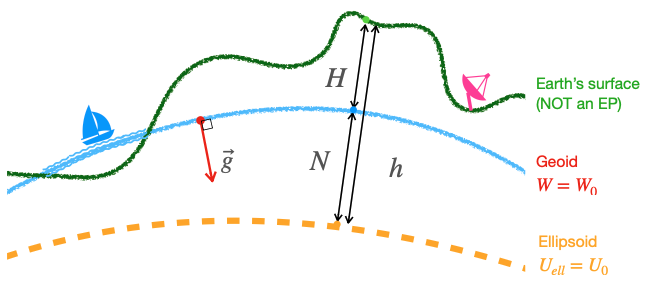
\includegraphics[width=0.7\linewidth]{fig/geoide02.png}
    \caption{Geoide e superficie della Terra. $H$ rappresenta l'altezza ortometrica.}
    \label{fig:geoide}
\end{figure}

\subsection{\textcolor{colore7}{Espansione armonica del potenziale gravitazionale}}

Dato che il potenziale gravitazionale è armonico fuori dalla Terra

\begin{equation}
    \nabla^2 W_g = 0
\end{equation}

\noindent
è conveniente esprimerlo in termini di funzioni armoniche sferiche.\\

\begin{figure}[!h]
    \centering
    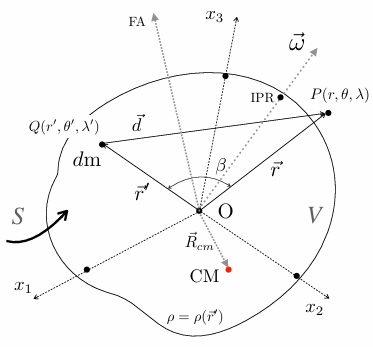
\includegraphics[width=0.5\linewidth]{fig/source_observer.png}
    \caption{Geometria del problema con osservatore e punto di massa.}
    \label{fig:source_observer}
\end{figure}

\noindent
Si consideri un corpo di densità arbitraria $\rho(\vec{x)}$, volume $V$ e superficie $S$ che ruota con velocità angolare $\vec{\omega} \parallel z$.
Il centro di massa \textit{CM} non coincide necessariamente con l'origine del sistema di riferimento \textit{O}.
Si considerino sulla superficie una massa puntiforme $dm = \rho(\vec{x})$ (sorgente) in $Q(r^\prime, \theta^\prime, \lambda^\prime)$, individuata dal vettore $\vec{r^\prime}$ e
una massa puntiforme (osservatore) $P(r, \theta, \lambda)$ individuata da $\vec{r}$. L'angolo tra le due è $\beta$.\\

\noindent
Vogliamo determinare il potenziale gravitazionale in \textit{P} dovuto a tutta la distribuzione di massa.\\

\noindent La distanza tra $P$ e $Q$ è ottenuta dal teorema di Carnot:

\begin{equation}
    \vec{d} = \vec{r} - \vec{r}' \longrightarrow \frac{1}{d} = \frac{1}{r} \sqrt{\frac{1}{1-2zcos\beta+z^2}}
\end{equation}

\noindent
con $cos\beta = cos\theta cos\theta' + sin\theta sin\theta ' cos(\lambda - \lambda')$.\\

\noindent Il potenziale gravitazionale in $P$ dovuto all'elemento di massa $dm$ è:

\begin{equation}
    dW_g = \frac{Gdm}{d}
\end{equation}

\noindent Grazie alla funzione generatrice dei polinomi di Legendre, si ottiene:

\begin{equation}
    dW_g = \frac{Gdm}{r} \sum_{l=0}^\infty \left( \frac{r'}{r} \right)^l P_l(cos\beta)
\end{equation}

\noindent Da cui, integrando su tutto il volume, si ricava l'\textit{espansione di multipolo} del potenziale gravitazionale esterno:

\begin{equation}
    W_g (r, \theta, \lambda) = \frac{G}{r} \sum_{l=0}^\infty \int_V \left( \frac{r'}{r} \right)^l P_l(cos\beta) dm
    \label{eq:gravitational_field_multipole}
\end{equation}

\noindent In tale espansione ($W_g (\vec{x}) = W_g^{(0)} (\vec{x}) + W_g^{(1)} (\vec{x}) + W_g^{(2)} (\vec{x}) + ...$), il multipolo di grado 0 rappresenta il potenziale di una massa puntiforme:

\begin{equation}
    W_g^{(0)}(\vec{x}) = W_g^{(0)}(r) = \frac{G}{r} \int_V dm = \frac{GM}{r}
\end{equation}

\noindent
ovvero il potenziale gravitazionale che osserveremmo in $r$ per una massa puntiforme $M$ o per una distribuzione di massa sferica simmetrica di pari massa.\\

I termini successivi rappresentano quindi le discrepanze dal potenziale sferico e decadono con potenze che dipendono dal grado $l$ ($\propto 1/r^{l+1})$.
La lunghezza d'onda spaziale di questi termini segue la regola di Jeans (vedi eq. \ref{eq:Jeans}).

\subsection{\textcolor{colore7}{Coefficienti di Stokes}}

Applicando il teorema di addizione (\ref{eq:addizione}) all'espansione di multipolo del campo gravitazionale nell'espressione ~\ref{eq:gravitational_field_multipole}, si ottiene un'espressione in cui non compaiono i polinomi di Legendre:

\begin{equation}
    P_l(cos\beta) = \frac{1}{2l+1} \sum_{m=-l}^l \mathcal{Y}^*_{lm} (\theta', \lambda') \mathcal{Y}_{lm}(\theta, \lambda)
\end{equation}

\noindent Confrontando con l'espansione in armoniche sferiche complesse si ricava:

\begin{equation}
    W_g (r, \theta, \lambda) = \frac{GM}{r} \sum_{lm} \left( \frac{a}{r} \right) ^l W_{g,lm} \mathcal{Y}_{lm} (\theta, \lambda)
\end{equation}

\noindent
dove compaiono i coefficienti complessi:

\begin{equation}
     W_{g,lm} = \frac{1}{M} \frac{1}{2l+1} \int_V \left( \frac{r'}{a} \right) ^l \mathcal{Y}^*_{lm} (\theta', \lambda') dm
\end{equation}

\noindent
dove $a$ è il raggio della Terra.
Questa espressione complessa si usa raramente, mentre la forma reale trova ampio utilizzo nella geodesia satellitare:

\begin{equation}
    W_g (r, \theta, \lambda) = \frac{GM}{r} \sum_{lm} \left( \frac{a}{r} \right) ^l (c_{lm} cos m\lambda + s_{lm} sin m\lambda) P_{lm}(cos \theta)
\end{equation}

\noindent
dove compaiono i \textbf{coefficienti di Stokes} $c_{lm}$ e $s_{lm}$ del campo gravitazionale, che dipendono dalla distribuzione di massa:

\begin{equation}
    \left\{ \begin{matrix}
        c_{lm} \\ s_{lm}
    \end{matrix}\right\} = (2-\delta_{0m}) \frac{(l-m)!}{(l+m)!} \frac{1}{M} \int_V \left( \frac{r'}{a} \right)^l P_{lm} (cos \theta) \left\{ \begin{matrix}
        cos m\lambda' \\ sin m\lambda'
    \end{matrix}\right\} dm
\end{equation}

\noindent
dove $l=0,1,2,\dots$ e $0 \leq m \leq l$. In base al grado si hanno coefficienti diversi: 

\begin{itemize}
    \item $l=0$: solo un coefficiente ($c_{00}$), è costante e indipendente dalla distribuzione di massa;
    \item $l=1$: tre coefficienti ($c_{10}, c_{11}, s_{11}$) associati alla scelta dell'origine del sistema di riferimento;
    \item $l=2$: cinque coefficienti ($c_{20}, c_{21}, c_{22}, s_{21}, s_{22}$) legati agli elementi del tensore di inerzia della distribuzione di massa.
\end{itemize}

\noindent
I coefficienti di grado basso dipendono dalla scelta del sistema di riferimento: se il centro di massa si trova nell'origine, allora i termini di grado 1 scompaiono.
Grazie ai satelliti, si cerca adesso di misurare la variazione nel tempo dei coefficienti di Stokes.\\

\noindent
Si consideri un corpo sfericamente simmetrico (Figura \ref{fig:stokes_a}):

\begin{figure}[!h]
    \centering
    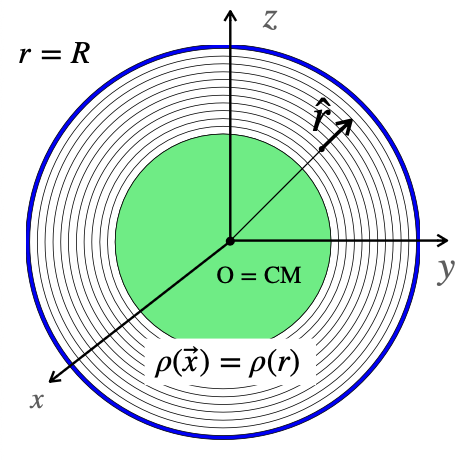
\includegraphics[width=0.35\linewidth]{fig/stokes_a.png}
    \caption{Distribuzione di massa sfericamente simmetrica.}
    \label{fig:stokes_a}
\end{figure}

\noindent
con densità $   rho(\vec x) = \rho(r)$ per $0 \leq r \leq R$.
Per questo corpo conosciamo la massa $M= 4\pi \int_0^R \rho(r) r^2 dr$, l'accelerazione di gravità
$\vec g (r) = - \frac{GM}{r^2} \hat{r}$ e il potenziale gravitazionale $W_g(r) = \frac{GM}{r}$.\\

\noindent
I coefficienti di Stokes sono: 

\begin{itemize}
    \item per $l=0$, $c_{00} = 1$, valido per tutti i corpi;
    \item per $l=1$, $c_{10} = c_{11} = s_{11} = 0$ perché $O=CM$;
    \item per $l\geq 3$, $c_{lm} = s_{lm} = 0$ perché l'unico termine di multipolo è quello di grado 0.
\end{itemize}

\noindent
Il momento di inerzia è dato da:

\begin{align}
    I &= \frac{1}{3}(I_{xx}+I_{yy}+I_{zz})=\frac{2}{3}\int_V(x^2+y^2+z^2)dm=\frac{2}{3}\int_Vr^4\rho(r)drsin\theta d\theta d\lambda \\ &=\frac{8\pi}{3}\int_0^Rr^4\rho(r)dr
\end{align}

\noindent
Per una massa omogenea vale:

\begin{equation}
    I_{hom} = \frac{8\pi}{15}R^5\rho_0
\end{equation}

\noindent
Dal confronto con il caso di una massa puntiforme si ricava il momento di inerzia medio normalizzato:

\begin{equation}
    \frac{I_{hom}}{MR^2} = \frac{2}{5}
\end{equation}

Nel caso della Terra si osserva che questo rapporto vale invece 0.33, per cui non è omogenea, ma c'è una concentrazione di massa al centro, a causa dell'autocompressione e della differenziazione chimica, che fanno aumentare la densità degli strati più profondi.

\subsection{\textcolor{colore7}{Ondulazioni del geoide}}

La forma della Terra è sferica in prima approssimazione, ma si può considerare anche un'ellissoide per maggiore precisione.
Gauss credeva di poterla descrivere attraverso un corpo molto regolare.
Introdusse così il \textbf{geoide}, cioè la superficie equipotenziale che intercetta la superficie degli oceani.\\

\noindent
Per misurare le irregolarità del geoide si considera un modello di Terra ideale (\textit{Terra normale}). Questa Terra:

\begin{itemize}
    \item è assisimmetrica;
    \item ruota con velocità angolare costante pari alla velocità angolare media terrestre;
    \item ha massa pari a quella terrestre;
    \item è un ellissoide a due assi;
    \item è definita da 4 parametri geometrici;
    \item ha un potenziale di gravità \textit{normale} dato da $U = U_g + U_c$, mentre il \textit{geoide normale} ha equazione $U=U_0$.    
\end{itemize}

\noindent
I 4 parametri geometrici sono $a, f, M, \omega$:

\begin{itemize}
    \item $a$: semiasse maggiore;
    \item $b$: semiasse minore;
    \item $f = \frac{a-b}{b}>0$: schiacciamento;
    \item $e^2 = \frac{a^2 - b^2}{a^2}$: eccentricità,
    \item $M$: massa;
    \item $\omega$: velocità angolare.
\end{itemize}

\noindent La differenza tra il campo di gravità del geoide e quello dell'ellissoide normale definisce le \textbf{ondulazioni del geoide}.

\begin{figure}[!h]
    \centering
    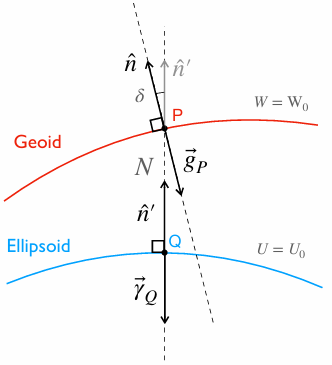
\includegraphics[width=0.5\linewidth]{fig/ondulazioni.png}
    \caption{Geometria della formula di Brun. 
    $P$ e $Q$ sono punti sulla superficie del geoide e dell'ellissoide, rispettivamente.}
    \label{fig:ondulazioni}
\end{figure}

\noindent
%Una piccola perturbazione rispetto al raggio terrestre data dalla :
Le ondulazioni del geoide sono date dalla \textit{formula di Brun}:

\begin{equation}
    N = \overline{PQ} = \frac{T_P}{\gamma_Q}
    \label{eq:Brun}
\end{equation}

\noindent
dove $T = W - U$ è il \textit{potenziale anomalo} e $\gamma$ è la gravità dell'ellissoide.
T può essere considerata una piccola perturbazione, dato che tutti gli ellissoidi "fittano bene" il geoide.
Quindi $N$ è una quantità piccola rispetto al raggio terrestre.\\

\noindent Si tratta della formula più importante della geodesia fisica.
Si ottiene a partire dalla definizione di derivata:

\begin{equation}
    U_P \simeq U_Q + \left( \frac{\partial U}{\partial n'} \right)_Q N
\end{equation}

\noindent Ma si ha il potenziale di gravità:

\begin{equation}
    \gamma_Q = - \left( \frac{\partial U}{\partial n'} \right)_Q
\end{equation}

\noindent Per cui vale:

\begin{equation}
    U_P \simeq U_Q - \gamma_Q N
\end{equation}

\noindent Da cui si ricava:

\begin{equation}
    \gamma_Q N = U_Q - U_P = (W_P - U_P ) - (W_P - U_Q) = T_P - (W_0 - U_0)
\end{equation}

\noindent La formula di Brun si ottiene ponendo in particolare $W_0 = U_0$.

\noindent L'ondulazione $N$ è proporzionale al potenziale di disturbo $T$ in $P$ rispetto al potenziale gravitazionale $\gamma$ in $Q$.\\

\begin{figure}[!h]
    \centering
    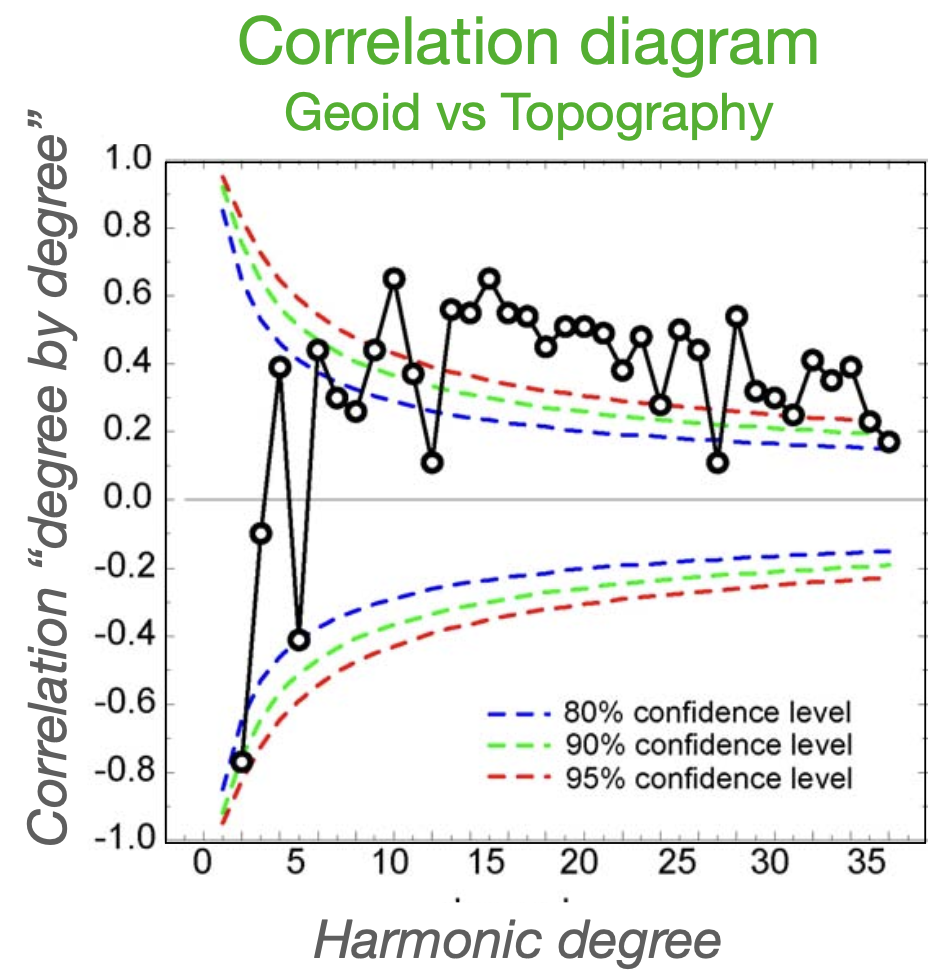
\includegraphics[width=0.45\linewidth]{fig/geoid_correlation.png}
    \caption{Diagramma di correlazione tra gradi armonici per geoide e topografia.}
    \label{fig:correlation}
\end{figure}

\noindent
Il potenziale $\gamma_Q$ è esprimibile come $\gamma_Q = \gamma_0 + \epsilon$, con $\gamma_0 = GM/R^2$ la gravità sulla superficie di una sfera di raggio $R$ (il raggio medio terrestre) e $\epsilon$ una quantità piccola $|\epsilon| \ll \gamma_0$. 
Questa approssimazione è detta \textit{approssimazione sferica}, segue che:

\begin{equation}
    N = \frac{T_P}{\gamma_0 + \epsilon} = \frac{T_P}{\gamma_0 (1 + \epsilon/\gamma_0)} \simeq \frac{T_P}{\gamma_0}(1 - \epsilon/\gamma_0)
\end{equation}

Dato che $T_P$ è una piccola perturbazione si ottiene di nuovo la formula di Brun (eq \ref{eq:Brun}).\\

\noindent
Grazie ai coefficienti di Stokes è possibile rappresentare $W_g$ e $U_g$ espandendoli in serie di armoniche sferiche reali e determinare che il geoide si discosta dall'ellissoide al massimo di un centinaio di metri.

\noindent
Le ondulazioni del geoide apparentemente non mostrano nessuna particolare simmetria o pattern.
La correlazione tra le ondulazioni e la topografia (Figura \ref{fig:correlation}) non è significativa per grandi lunghezze d'onda ($l < 12$), diventa invece significativa per lunghezze d'onda più corte ($l > 12$).
A grande scala il geoide sente l'effetto delle anomalie di densità associate alla dinamica interna della Terra; a piccola scala, invece, riflette i processi superficiali.

\newpage

\section{\textcolor{colore2}{Criosfera}}

Si tratta dell'insieme di tutti i ghiacci presenti sulla Terra, una volta considerati parte dell'idrosfera.
È una componente estremamente sensibile ai cambiamenti climatici ed evolve molto rapidamente.
Interagisce fortemente con il clima ed è un'importante fonte di acqua dolce.
Le masse glaciali esercitano un carico sulla Terra ed un'attrazione gravitazionale con gli oceani.
La forma degli oceani determina la pressione sui fondali e il potenziale centrifugo.

\subsection{\textcolor{colore2}{Acqua e ghiaccio}}

L'acqua ricopre il 71\% della superficie terrestre.

\begin{itemize}
    \item Il 96.5\% si trova in mari e oceani;
    \item l'1.7\% nelle acque sotterranee;
    \item l'1.7\% nei ghiacciai;
    \item lo 0.001\% in atmosfera sottoforma di vapore, nubi o precipitazione.
\end{itemize}

Solo il 2.5\% dell'acqua sulla Terra è dolce e il 98.8\% di essa si trova nel ghiaccio e nel suolo.
Meno dello 0.3\% dell'acqua dolce si trova nei fiumi, laghi e nell'atmosfera.\\

\noindent
L’origine dell’acqua sulla Terra è ancora un problema aperto: le comete da sole non sembrano spiegare interamente la presenza degli oceani.
Un ruolo importante potrebbe essere stato ricoperto dai meteoriti e dai planetesimi ghiacciati durante l’intenso bombardamento tardivo ($\approx 700$ milioni di anni dopo la formazione della Terra), anche se studi recenti suggeriscono che parte dell’idrogeno necessario alla formazione dell’acqua fosse già presente all’interno della Terra primordiale.\\

Il ciclo dell'acqua descrive il continuo movimento dell’acqua sulla superficie terrestre, nell’atmosfera, nel sottosuolo e anche tra l’interno della Terra e lo spazio esterno.
Sebbene la quantità totale di acqua sulla Terra rimanga quasi costante nel tempo, la sua distribuzione tra oceani, ghiacci, acque dolci e atmosfera varia in funzione delle condizioni climatiche.
Il ciclo dell’acqua influisce inoltre sulla convezione del mantello e quindi sulla tettonica delle placche.

\subsection{\textcolor{colore2}{Componenti della criosfera}}

Dalla IPCC del 2007 si distinguono i \textit{ghiacciai}, che permettono di determinare la topografia sottostante, dalle \textit{lenzuola glaciali}, che la nascondono completamente.

Lo spessore della neve è nell'ordine di un metro, mentre il ghiaccio marino generalmente arriva a qualche metro; i ghiacciai alpini hanno uno spessore di alcune decine di metri, le piattaforme glaciali anche 200 metri.
Lo spessore del ghiaccio nelle lenzuola glaciali si misura spesso in km, tanto da abbassare per via di processi isostatici la crosta terrestre.

In base allo spessore cambia anche la scala temporale di variabilità, da pochi giorni per la neve, agli anni per i ghiacciai, alle centinaia di migliaia di anni per le calotte glaciali (Figura \ref{fig:cryosphere_scales}).

\begin{figure}[!h]
    \centering
    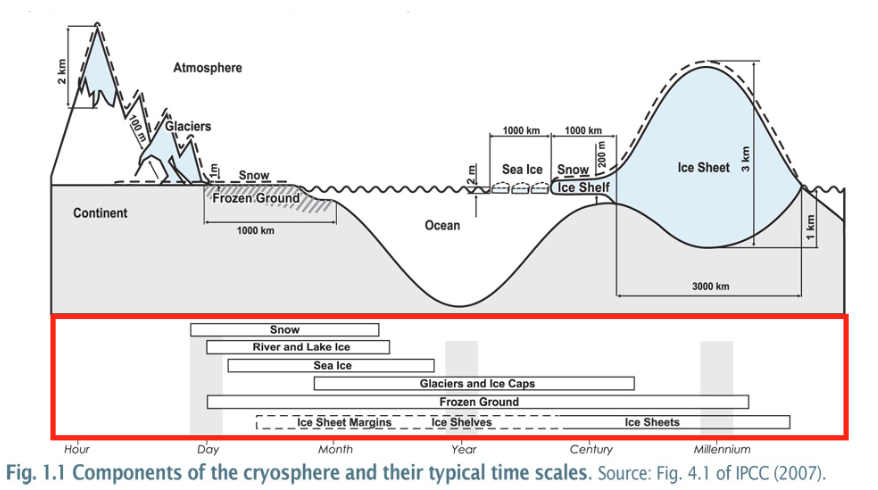
\includegraphics[width=0.75\linewidth]{fig/cryosphere_scales.png}
    \caption{Scale spaziali e temporali delle componenti della criosfera.}
    \label{fig:cryosphere_scales}
\end{figure}

\subsubsection{\textcolor{colore2}{Neve}}

La neve rappresenta la componente della criosfera con la maggiore estensione geografica, arrivando a coprire circa 50 milioni di $km^2$ nell'emisfero settentrionale durante i mesi invernali.
Si origina come cristalli di ghiaccio all'interno di nubi con temperature inferiori agli $0^\circ$C e precipita in forme variegate come fiocchi (aggregati di cristalli), grandine e nevischio.\\

\noindent
Una volta depositata al suolo, la neve evolve in base alla densità e al tempo di permanenza.
Con neve compatta (\textit{firn}) si fa riferimento alla neve che ha resistito per più di un anno, raggiungendo una densità superiore ai 550 $kg/m^3$.
Altre tipologie sono la neve sciolta (slush) o i sastrugi.\\

\noindent
L'estensione della neve ha conseguenze dirette sul bilancio energetico del pianeta.
Dato il suo alto albedo, la neve riflette la maggior parte della radiazione solare, contribuendo a mantenere basse le temperature superficiali.
Al contempo, la sua bassa conducibilità termica funge da isolante per il terreno, proteggendo il suolo dalle rigide temperature invernali.

Infine, la capacità della neve di uniformare le irregolarità del terreno riduce la resistenza al vento e modifica gli scambi energetici con l'atmosfera.
Queste interazioni locali e regionali influenzano pesantemente il budget energetico della terra alla superficie, con efetti che si propagano influenzando la circolazione atmosferica globale.

\subsubsection{\textcolor{colore2}{Ghiaccio marino}}

Il ghiaccio marino ha origine direttamente dal congelamento della superficie oceanica.
A causa della salinità, questo processo richiede temperature inferiori rispetto allo zero termico dell'acqua dolce, innescandosi solitamente intorno ai $-1.8^\circ$C.
Nonostante il suo spessore limitato, che varia da pochi centimetri a pochi metri, la sua influenza sul sistema climatico è significativa.\\

\noindent
La classificazione del ghiaccio marino dipende dall'età, dallo spessore e dalla forma.
Si passa dalle fasi iniziali come il \textit{nials} (uno strato sottile inferiore ai 10 cm) al ghiaccio grigio, fino ad arrivare al ghiaccio del primo anno (\textit{first-year ice}), che può raggiungere i 1.8 metri.
Il ghiaccio pluriennale, ovvero quello che è sopravvissuto ad almeno una stagione di fusione estiva, è più denso e strutturato.\\

\noindent
Il ghiaccio marino funge da "coperta termica" globale, isolando l'oceano dall'atmosfera e limitando lo scambio di calore e umidità.
Un contributo fondamentale riguarda l'albedo: la sua superficie brillante riflette più radiazione solare rispetto agli oceani, contribuendo a mantenere fresche le regioni polari.
Quindi, lo scioglimento del ghiaccio marino innesca un feedback positivo: il calore assorbito comporta una diminuzione della superficie riflettente, accelerando ulteriormente il riscaldamento nelle alte latitudini.\\

\noindent
Le osservazioni satellitari effettuate a partire dal 1979 mostrano che l'estensione minima del ghiaccio artico, che viene raggiunta ogni settembre, sta diminuendo al ritmo del 13.2\% per decennio.

\begin{figure}[!h]
    \centering
    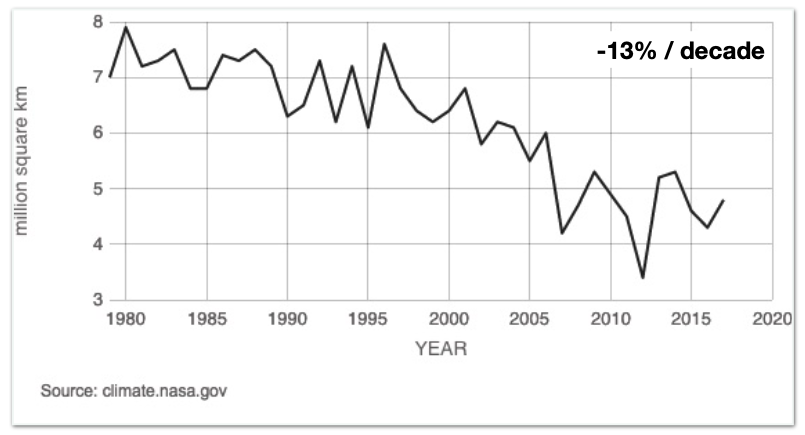
\includegraphics[width=0.55\linewidth]{fig/artic_sea_minimum.png}
    \caption{Estensione media mensile del ghiaccio marino.}
\end{figure}

\subsubsection{\textcolor{colore2}{Permafrost}}

Il permafrost è definito come terreno la cui temperatura rimane pari o inferiore a 0 °C per almeno due anni consecutivi.
La sua identificazione si basa esclusivamente su criteri termici: l'acqua ghiacciata può essere presente, ma non è una condizione necessaria per la sua classificazione.
Questa componente della criosfera è ampiamente diffusa nelle regioni artiche e subartiche, nelle zone montuose d'alta quota e le regioni prive di ghiaccio dell'Antartide.
Nell'emisfero nord, il permafrost interessa circa 23 milioni di $km^2$, un'area superiore a due volte la superficie degli Stati Uniti continentali.\\

\noindent
Dal punto di vista strutturale, il permafrost può essere continuo, discontinuo, sporadico e isolato.
Come evidenziato dai profili termici, si distinguono diverse zone:

\begin{itemize}
    \item Strato attivo (\textit{active layer}): è la porzione più superficiale, soggetta a forti fluttuazioni stagionali. Questo strato fonde durante l'estate e congela in inverno, quindi è più reattivo alle variazioni di temperatura stagionali;
    \item Permafrost: situato al di sotto dello strato attivo, risponde a variazioni termiche su scala decennale. A causa della bassa velocità di conduzione del calore nel terreno, le variazioni interannuali della temperatura dell'aria vengono mediate, rendendo questa zona un indicatore sensibile dei trend climatici a lungo termine;
    \item Talik: porzioni di terreno non ghiacciato che possono trovarsi all'interno o alla base del permafrost.
\end{itemize}

\noindent
La sua importanza per il sistema Terra è cruciale a causa del carbonio intrappolato al suo interno: si stima che contenga circa 1400 Gt di carbonio, quasi il doppio di quanto sia attualmente presente nell'intera atmosfera terrestre.
Lo Yedoma è un tipo di permafrost risalente al Pleistocene ricco di carbonio, situato in Russia e Siberia. Si stima che un aumento della temperatura globale di $1.5^\circ$C rispetto ai livelli attuali sarebbe sufficiente per innescarne il disgelo.

\subsubsection{\textcolor{colore2}{Ghiacciai}}

I ghiacciai sono grandi masse di ghiaccio in movimento, nate dalla stratificazione e compattazione della neve, che fluiscono lentamente sotto l'effetto della gravità e della pressione interna.
Costituiscono la più grande riserva di acqua dolce del pianeta, e sono secondi solo agli oceani per riserva di acqua totale.\\

\noindent
I ghiacciai si formano a partire da precipitazioni nevose persistenti a temperature inferiori al punto di congelamento per gran parte dell'anno.
Attraverso un processo di \textit{pressure sintering}, i cristalli di neve accumulati si fondono nei punti di contatto, espellendo l'aria e aumentando progressivamente la densità.
Nelle regioni più fredde, come l'Antartide centrale, dove le precipitazioni sono scarse e la fusione quasi assente, questa trasformazione in ghiaccio glaciale può richiedere da secoli a millenni.\\

\noindent
Si categorizzano in base alla morfologia, alle caratteristiche termiche e al comportamento.
Alcuni raggiungono velocità di alcuni metri al giorno.

\begin{itemize}
    \item Ghiacciai alpini: ricoprono montagne e valli;
    \item Calotte glaciali (\textit{ice caps}): hanno estensione inferiore a 50'000 $km^2$ e si trovano in regioni montuose;
    \item Lenzuola glaciali (\textit{ice sheets}): hanno estensione superiore a 50'000 $km^2$. I soli due esempi esistenti sono quelli che coprono Antartide e Groenlandia.
    \item Piattaforme glaciali (\textit{ice shelves}): porzioni di ghiaccio che galleggiano sull'acqua;
    \item Correnti glaciali (\textit{ice streams}): sezioni delle lenzuola glaciali che raggiungono la massima velocità.
\end{itemize}

\noindent
La perdita di massa per fusione o distacco dei ghiacciai è detta \textit{ablazione} e si monitora per studiare il bilancio di massa, grazie anche a fotografie storiche.
Se l'accumulo di massa supera l'ablazione, il ghiacciaio avanza; in caso contrario, si osserva un ritiro.\\

\noindent
Sebbene i ghiacciai rappresentino solo lo 0,5\% del ghiaccio terrestre totale, il loro scioglimento ha contribuito all'innalzamento del livello del mare nel secolo scorso in misura maggiore rispetto alle lenzuola glaciali.\\

\noindent
Questi sistemi sono monitorati costantemente, anche attraverso ghiacciai "benchmark" come quello sul Monte Rainier, poiché fungono da indicatori delle variazioni climatiche globali.\\

\noindent
L'estensione dei ghiacciai segue cicli di lungo periodo, stimati in circa 90 mila anni, legati alle variazioni dell'orbita terrestre e dell'irradiazione solare.\\

\noindent
I ghiacciai sono corpi mobili dotati di una propria dinamica interna.
Il movimento avviene principalmente attraverso due meccanismi:

\begin{itemize}
    \item Deformazione plastica: a profondità elevate, la pressione degli strati superiori induce il ghiaccio a comportarsi come un materiale plastico, permettendogli di scorrere lentamente;
    \item Scorrimento basale: quando alla base del ghiacciaio è presente acqua liquida, la massa può scivolare sul letto roccioso. Se invece il ghiaccio è congelato direttamente al suolo, la velocità alla base è nulla.
\end{itemize}

\noindent
L'attrito esercitato dalle pareti delle valli e dal letto roccioso rallenta il flusso ai bordi e sul fondo.
Di conseguenza, la velocità è massima verso il centro della massa.
Sebbene la velocità media si misuri in metri all'anno, alcuni ghiacciai si muovono appena nel corso di un decennio; in altri casi i ghiacciai possono andare incontro a surge improvvisi, raggiungendo spostamenti di decine di metri al giorno.

\subsubsection{\textcolor{colore2}{Lenzuola (o scudi) glaciali}}

Si tratta di ghiacciai con un'estensione superficiale superiore a 50'000 $km^2$ che nascondono completamente la topografia sottostante.
Attualmente, gli unici scudi glaciali esistenti ricoprono la Groenlandia e l'Antartide.\\

\noindent
Si formano in migliaia di anni per accumulo di ghiaccio e la compattazione della neve.
Dall'ultimo massimo glaciale tre lenzuola glaciali si sono completamente sciolte: Laurentide (Nord America), Weichselian (Europa settentrionale) e Patagonia.
In tale periodo esistevano molti ponti di ghiaccio che permisero lo spostamento degli umani attraverso diversi continenti.\\

\begin{figure}[!h]
    \centering
    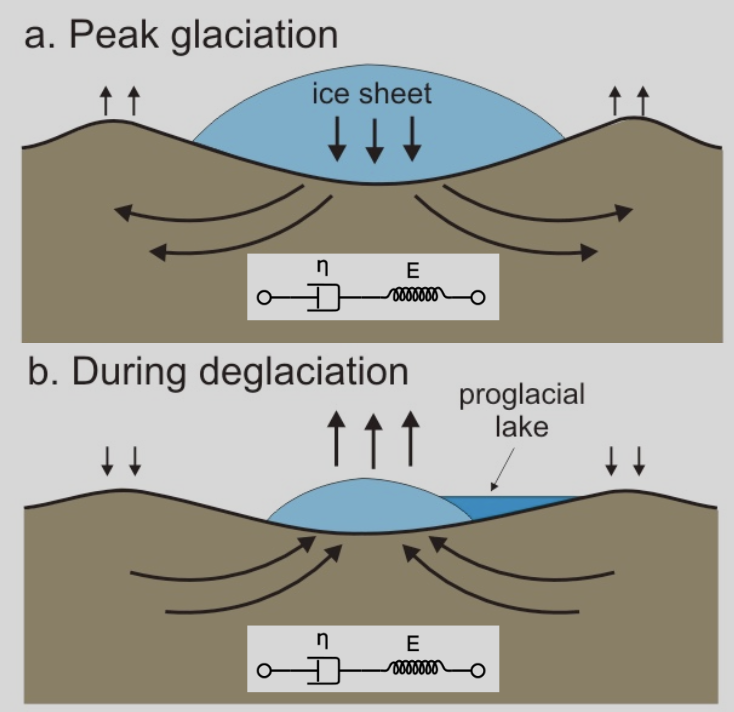
\includegraphics[width=0.4\linewidth]{fig/rimbalzo.png}
    \caption{Le due fasi del rimbalzo post-glaciale.}
    \label{fig:rimbalzo}
\end{figure}

\noindent
Il peso di queste masse esercita una pressione tale da deformare la crosta terrestre.
Questo fenomeno, noto come Aggiustamento Isostatico Glaciale (o rimbalzo post-glaciale) rivela come la Terra si comporti come un corpo reologico di Maxwell (Figura \ref{fig:rimbalzo}):

\begin{itemize}
    \item Fase di picco glaciale (comportamento elastico): la superficie terrestre sprofonda sotto il carico del ghiaccio e si solleva leggermente nelle aree periferiche a causa del flusso del mantello.
    \item Fase di deglaciazione (comportamento viscoso): con lo scioglimento dei ghiacci, la regione depressa inizia a risalire lentamente mentre le zone periferiche sussidono.
\end{itemize}

\noindent
La Groenlandia e l'Antartide presentano dinamiche di perdita di massa (ablazione) differenti:

\begin{itemize}
    \item Groenlandia: se fusa completamente, innalzerebbe il livello del mare di circa 7 metri.
    L'ablazione è dominata dallo scioglimento superficiale e basale vicino alle coste.
    Le tecniche gravimetriche indicano una perdita di massa di circa $286 \pm 21$ Gt all'anno.
    \item Antartide: ha un livello marino equivalente di 58 metri.
    La perdita di massa avviene principalmente tramite \textit{calving} (distacco di iceberg).
    La perdita di massa stimata è di circa $127 \pm 39$ Gt all'anno.
\end{itemize}

\noindent
In Antartide la Catena Transantartica (che si sviluppa tra il Mare di Ross e il Mare di Weddell) separa l'Antartide Orientale dall'Antartide Occidentale, dove si trova la ben studiata Penisola Antartica.
Al di sotto si trovano almeno 600 laghi subglaciali.\\

\noindent
La stabilità delle lenzuola glaciali è strettamente legata alla lubrificazione della loro base.
La \textit{grounding line} (linea di galleggiamento) individua il confine dove il ghiaccio smette di poggiare sul letto roccioso e inizia a galleggiare.
La modellizzazione attuale presenti dei limiti: spesso le lenzuola glaciali sono trattate come condizioni al contorno di sforzo normale, senza tenere conto della reologia del ghiaccio.\\

\noindent
Le lenzuola glaciali sono importanti archivi climatici.
Le carote di ghiaccio permettono di ricostruire la composizione atmosferica e le temperature di centinaia di migliaia di anni fa.

\subsubsection{\textcolor{colore2}{Piattaforme glaciali}}

Sono piattaforme galleggianti di ghaiccio permanente, collegate alla terraferma, che si propagano nell'oceano a partire dalle lenzuola polari.
A differenza del ghiaccio marino (sea ice), le piattaforme glaciali sono costituite da ghiaccio d'acqua dolce proveniente dalla terraferma.\\

\noindent
Si trovano prevalentemente in Antartide, ma sono presenti anche in Groenlandia e nel Canada artico.
Hanno estensioni di migliaia di $km^2$ e spessori di centinaia di metri. In Groenlandia, la quasi totalità del loro spessore rimane immersa sott'acqua.
Galleggiano sull'acqua dell'oceano, formando una barriera tra quest'ultimo e le lenzuola glaciali.
L'acqua liquida che scorre al di sotto favorisce lo scorrimento del ghiaccio verso l'oceano e il calving.\\

\noindent
Il processo di perdita di massa naturale è il calving, ovvero il distacco di iceberg dal fronte della piattaforma.
L'equilibrio della piattaforma è però estremamente sensibile alle variazioni termiche:
in condizioni di stabilità, la spinta idrostatica sostiene la piattaforma e questa limita il flusso del ghiacciaio per gravità;
l'aumento delle temperature provoca la percolazione dell'acqua nelle fratture del ghiacciaio, accelerando la disintegrazione della piattaforma.
Quando una piattaforma si ritira oltre la \textit{grounding line}, il supporto idrostatico diminuisce. Il ghiacciaio continentale subisce una rapida accelerazione e un assottigliamento, riversando masse di ghiaccio nell'oceano.

\begin{figure}[!h]
    \centering
    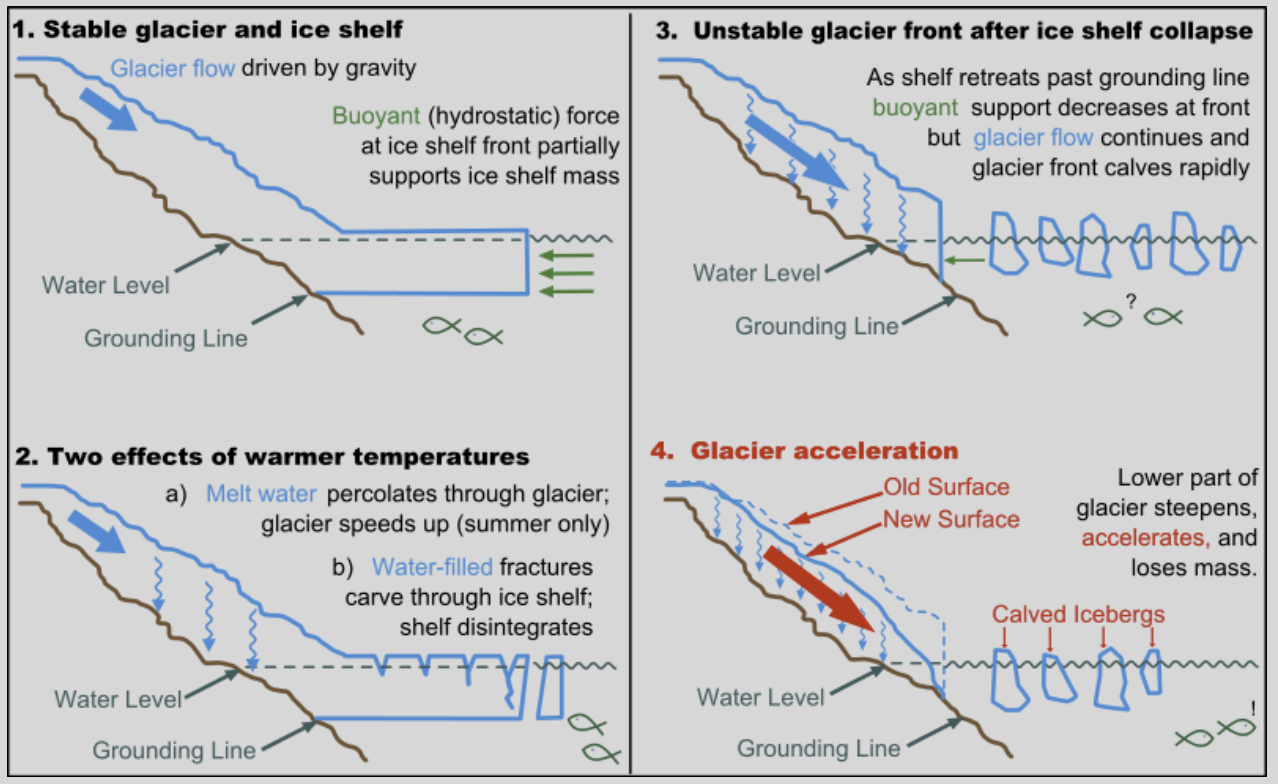
\includegraphics[width=0.5\linewidth]{fig/ice_shelves.png}
    \caption{Processo di \textit{calving} di una piattaforma glaciale.}
    \label{fig:ice_shelf}
\end{figure}

\noindent
La fusione delle piattaforme ghiacciate ha due contributi:

\begin{itemize}
    \item Impatto diretto: poiché le piattaforme galleggiano, la loro fusione contribuisce minimamente all'innalzamento del livello del mare (si stima circa 4 cm se fondessero tutte le piattaforme esistenti);
    \item Impatto indiretto: la rimozione delle piattaforme permette ai ghiacciai continentali (che poggiano sulla terraferma) di fluire molto più velocemente verso l'oceano. Questo nuovo volume di ghiaccio, spostandosi da sopra il livello del mare, contribuisce significativamente all'innalzamento dei mari.
\end{itemize}

\subsection{\textcolor{colore2}{Groenlandia}}

La geofisica moderna nacque a seguito degli studi condotti in Groenlandia dal fisico e meteorologo tedesco Alfred Wegener.
Circa 130'000 anni fa la Groenlandia non era ricoperta dai ghiacci. 
Fu scoperta attorno all'anno 1000 (quando la temperatura media globale era maggiore di quella attuale) dal vichingo Erik il Rosso, che esplorò anche la costa occidentale e favorì la nascita di diversi insediamenti.

Il ghiacciaio di Jackobshavn, vicino alla città di Ilulissat, nella Baia di Disko, mostra una ritirata estremamente rapida: il \textit{calving front} avanza di diversi chilometri all'anno verso l'entroterra.

Il centro della Groenlandia è costituito da un cratone molto stabile che si trova sotto il livello del mare, su cui poggiano oltre 3 km di ghiaccio.
Sono presenti pochi laghi subglaciali, grazie anche alla presenza del canyon più lungo del mondo, che drenando l'acqua potrebbe aver aumentato la stabilità del ghiaccio soprastante.

Attualmente la Groenlandia perde circa 8'500 tonnellate di ghiaccio ogni secondo, ma negli ultimi 20'000 anni si sono alternate diverse fasi di riscaldamento e raffreddamento.
Durante l'evento del \textit{Younger Dryas}, circa 12'000 anni fa, lo scioglimento del ghiacciaio di Laurentide, in Nord America, comportò il rilascio di un'enorme quantità di acqua fredda, che sconvolse la circolazione oceanica, interrompendo per diverse migliaia di anni il generale processo di riscaldamento che la Terra stava attraversando.

La missione \textit{IceBridge} della NASA monitora il ghiaccio marino e continentale grazie a dei voli condotti sopra la Groenlandia e parte dell'Antartide.
Grazie a dei radar sono stati misurati gli strati ghiacciati a diverse latitudini e profondità.

\subsubsection{\textcolor{colore2}{Modellazione delle deformazioni elastiche in atto in Groenlandia}}

\textit{ICESat} (\textbf{I}ce, \textbf{C}oud, and Land \textbf{E}levation \textbf{Sat}ellite) è un satellite della NASA che dal 2003 monitora il bilancio di massa e la distribuzione topografica dei ghiacci in Groenlandia con una risoluzione di 5 km $\times$ 5 km.
Si è misurata una diminuzione dell'altezza del ghiaccio di circa 3 m all'anno in alcune zone vicine alla costa e un aumento in zone più centrali (a causa del recente aumento delle nevicate).
Il bilancio complessivo è fortemente negativo e sta peggiorando in fretta ($-240 \pm 28$ Gt/y, dove 360 Gt di ghiaccio determinano un aumento del livello marino di 1 mm).

Grazie ai dati forniti dal satellite, è possibile modellare la risposta alla fusione del ghiaccio grazie al codice di calcolo $REAR$ (\textbf{R}egional \textbf{E}l\textbf{a}stic \textbf{R}ebound calculator).
A seguito dell'applicazione di un carico come un Mascon si osservano le seguenti risposte:

\begin{itemize}
    \item lo spostamento verticale è sempre negativo e raggiunge l'entità massima sotto al carico;
    \item lo spostamento orizzontale è rivolto verso il centro del disco e raggiunge il massimo nei pressi del bordo;
    \item l'altezza del geoide aumenta ovunque, ma in maniera più evidente nei pressi del Mascon.
\end{itemize}

La Groenlandia subisce un sollevamento geodetico di circa 18 mm/y nei pressi delle coste, maggiore dell'innalzamento del livello marino.
Mentre per alcuni processi di breve durata è possibile utilizzare un modello elastico, per altri, di maggiore durata, è necessario tenere in considerazione la risposta viscoelastica.

\newpage

\section{\textcolor{colore7}{\textcolor{colore7}{Reologia I}}}

\subsection{\textcolor{colore7}{Movimenti incessanti nel Sistema Terra}}

I movimenti della Terra sono testimoniati dai terremoti, manifestazioni di onde elastiche regolate dall'\textit{equazione d'onda di Newton}, alla base della sismologia:

\begin{equation}
    \rho \frac{\partial^2 \vec{u}}{\partial t^2} = \left( K + \frac{4}{3} \mu \right) \nabla (\nabla \cdot \vec{u}) - \mu \nabla \times (\nabla \times \vec{u})
    \label{eq:onda}
\end{equation}

A causa della complessità dell'interno della Terra, la diffusione delle onde sismiche non è banale.
Siccome hanno un periodo caratteristico di pochi secondi, permettono di sondare il pianeta ad alta frequenza, alla quale il mantello appare solido.
Terremoti particolarmente energetici fanno assumere alla Terra vibrazioni in moti sferici, che ne cambiano la forma, e toroidali, che causano torsione, dissipando energia (oscillazioni libere). 
Il tempo caratteristico di queste oscillazioni è di decine di minuti.
Furono misurate per la prima volta a seguito del terremoto del Cile del 1960.

I moti mareali hanno periodi semidiurni, diurni e annuali e sono dovuti alla non uniformità dei campi gravitazionali.
Causano anche le correnti oceaniche.
La Terra risponde in maniera elastica.

\subsection{\textcolor{colore2}{Reologia e Scienze della Terra}}

La \textbf{reologia} nacque per studiare il fluire delle lave, ma si applica anche a ghiacciai, livello del mare, deformazioni post-sismiche, isostasia glaciale e tettonica delle placche.
Il termine deriva dal greco e indica lo studio di flussi e deformazioni dei materiali.\\

\noindent
Il concetto di corpo rigido fu introdotto da Archimede, ma trova la sua formalizzazione matematica con Newton nel 1687.
Hooke definì le basi dell'elasticità (1678), mentre Bernoulli ed Eulero iniziarono a descrivere i fluidi invisicidi (1800s).
Successivamente furono studiati fluidi e materiali viscoelastici, fino all'avvento della reologia nel 1929.\\

\noindent
Einstein trovò una formula per descrivere la viscosità di una sospensione diluita di particelle in un fluido di viscosità iniziale $\eta_m$:

\begin{equation}
    \frac{\eta}{\eta_m} = 1 + \frac{5}{2} c \text{ , dove c $\ll$ 1 è la concentrazione}
\end{equation}

\noindent
In reologia la definizione di materiale solido o fluido non è fatta in base alla sua struttura atomica,
bensì un materiale è definito fluido se fluisce quando sottoposto ad uno stress costante.
La fluidità quindi non è una proprietà intrinseca del materiale, ma dipende da fattori esterni come la temperatura, la pressione e il tempo di carico.\\

\noindent
Si hanno due approcci fondamentali allo studio della reologia:

\begin{itemize}
    \item Meccanica dei continui (macroreologia): le proprietà dei materiali sono descritte in maniera fenomenologica,
    ignorando la natura corpuscolare e descrivendo il comportamento macroscopico;
    \item Fisica dello stato solido (microreologia): considera la microfisica, e le proprietà a livello atomico, in maniera complementare al primo approccio.
\end{itemize}

La reologia studia i materiali con caratteristiche sia solide che fluide, mettendo in relazione \textit{stress} e \textit{strain}.

Si può descrivere la struttura interna della Terra sulla base di una stratificazione chimica (crosta, mantello e nucleo) o reologica (litosfera, astenosfera, mesosfera, nucleo esterno e nucleo interno).
La stratificazione chimica è studiata grazie alla sismologia, mentre quella reologica grazie a processi tettonici e dall'isostasia.

\subsection{\textcolor{colore7}{Equazioni reologiche costitutive}}

Le grandezze cinematiche e dinamiche di base della reologia sono, rispettivamente, lo strain (o \textit{strain rate}) $\varepsilon$, che generalizza il concetto di spostamento o deformazione,
e lo stress, o sforzo, $\sigma$, che generalizza il concetto di forza agente sul corpo, entrambi tensori cartesiani di rango 2.

Traslazioni e rotazioni, quindi operazioni che non causano deformazioni, non sono investigate dalla reologia.

Altri parametri o proprietà intrinseche dei materiali comprendono rigidità, comprimibilità e viscosità.
Questi sono detti \textit{parametri materiali} (di natura tensoriale) e il loro valore dipende dalle condizioni esterne.
Anche il tipo di comportamento reologico può differire al variare delle condizioni esterne.\\

\noindent
La forma generale delle equazioni costitutive mette in relazione le quantità cinematiche e dinamiche attraverso dei parametri materiali, come si osserva nell'\textit{equazione di stato reologica}:

\begin{equation}
    R(\varepsilon, \dot{\varepsilon}, \ddot{\varepsilon}, ...; \sigma, \dot{\sigma}, \ddot{\sigma}, ...; \{M\} ) = 0
    \label{eq:reologia}
\end{equation}

\noindent
dove $R$ rappresenta la funzione reologica, $\varepsilon$ lo strain, $\sigma$ lo stress ed $\{M\}$ il vettore di parametri materiali.
Queste relazioni si ottengono da evidenze sperimentali e da principi fisici.
La classificazione di un materiale in classi reologiche (come elstico, plastico o viscoso) riflette il tipo di equazione reologica che lo descrive.
Si distinguono diversi comportamenti reologici.

\begin{table}[h]
    \centering
    \renewcommand{\arraystretch}{1.5}
    \setlength{\tabcolsep}{12pt}
    \begin{tabular}{|c|c|c|}
        \hline
        $F=-kx$ & Legge delle molle & Elasticità lineare \\ 
        \hline
        $F_{attrito}=\mu N$ & Legge di Amonton & Attrito \\ 
        \hline
        $\sigma_{ij}=C_{ijkl}\varepsilon_{kl}$ & Legge di Hooke (3D) & Elasticità tridimensionale \\ 
        \hline
        $\sigma=C\varepsilon$ & Legge di Hooke (1D) & Elasticità monodimensionale \\ 
        \hline
        $\vec{J}=-\boldsymbol{D}\nabla c$ & Legge di Fick & Diffusione \\ 
        \hline
        $q=-\frac{k}{\mu}\Delta P$ & Legge di Darcy & Flusso in mezzo poroso \\ 
        \hline
        $V=RI$ & Legge di Ohm & Circuiti elettrici \\ 
        \hline
    \end{tabular}
\end{table}

\noindent
$C_{ijkl}$ è il tensore delle costanti elastiche.

\subsection{\textcolor{colore7}{Esperimenti meccanici ideali}}

Sono esperimenti in cui stress o strain cambiano nel tempo in modo tale da manifestare l'equazione costitutiva che caratterizza il materiale.

\subsubsection{\textcolor{colore7}{Creep test}}

Si applica uno stress costante $\sigma_0$ al tempo $t=0$.
Lo stress $\sigma (t)$ è quindi descritto tramite la \textit{funzione di Heaviside}:

\begin{equation}
    \sigma(t) = \sigma_0 H(t) \text{ , dove } H(t) \equiv \begin{cases}
        0 & se \text{  } t \le 0 \\ 1 & se \text{  } t > 0
    \end{cases}
\end{equation}

\noindent
In risposta al carico lo strain aumenta nel tempo, mentre il materiale striscia.

\noindent In un esperimento di creep si osservano tre fasi:

\begin{itemize}
    \item \textit{creep primario}, transiente, in cui $\dot{\varepsilon}$ varia nel tempo;
    \item \textit{creep secondario}, stazionario, in cui $\dot{\varepsilon}$ resta costante;
    \item \textit{creep terziario}, che precede la rottura.
\end{itemize}

\begin{figure}[htbp]
    \centering
    \begin{minipage}{0.25\textwidth}
    \centering
    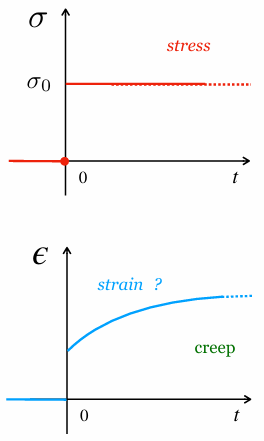
\includegraphics[width=\linewidth]{fig/creep_test.png}
    \caption{Creep test.}
    \label{fig:creep_test}   
    \end{minipage}
    \hfill
    \begin{minipage}{0.65\textwidth}
    \centering
    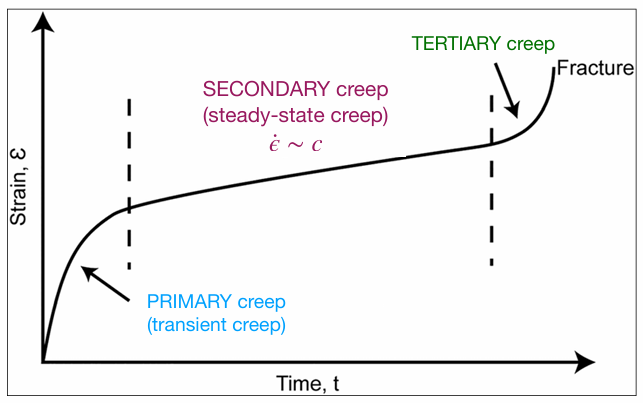
\includegraphics[width=\linewidth]{fig/creep_strain.png}
    \caption{Esempio di \textit{curva di creep}: deformazione sotto stress costante in un creep test.}
    \label{fig:creep_strain}    
    \end{minipage}
\end{figure}

\subsubsection{\textcolor{colore7}{Relaxation test}}

Si applica uno strain costante $\varepsilon_0$ al tempo $t=0$ e si misura la diminuzione dello stress, mentre il materiale si rilassa.

\begin{equation}
    \varepsilon(t) = \varepsilon_0 H(t) \text{ , dove } H(t) \equiv \begin{cases}
        0 & se \text{  } t \le 0 \\ 1 & se \text{  } t > 0
    \end{cases}
\end{equation}

\begin{figure}[H]
    \centering
    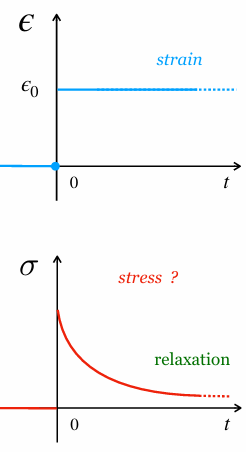
\includegraphics[width=0.5\linewidth]{fig/relaxation_test.png}
    \caption{Relaxation test.}
    \label{fig:relaxation_test}
\end{figure}

\noindent
Generalmente si osserva un decadimento dello stress, ma non necessariamente questo è esponenziale.

\subsubsection{\textcolor{colore7}{Loading/Unloading test}}

Si applica uno stress costante $\sigma_0$ per un periodo finito $T$ e si misura lo strain variabile durante e dopo.

\begin{equation}
    \sigma(t) = \sigma_0 (H(t-t_1) - H(t-t_2))
\end{equation}

\begin{figure}[H]
    \centering
    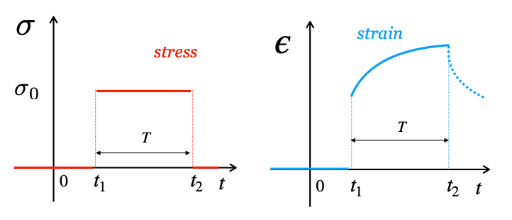
\includegraphics[width=0.5\linewidth]{fig/LU_test.png}
    \caption{Loading/Unloading test.}
\end{figure}

\subsubsection{\textcolor{colore7}{Dynamic test}}

Si applica uno stress che oscilla nel tempo secondo una funzione armonica e si misurano la differenza di fase tra stress e strain, associato alla dissipazione di energia.

\begin{equation}
    \sigma(t) = H(t) sin (\omega t + \varphi) \text{ , dove } \omega = \frac{2\pi}{T} \text{ è la frequenza, } T \text{ è il periodo e } \varphi \textit{ è la fase}
\end{equation}

\begin{figure}[H]
    \centering
    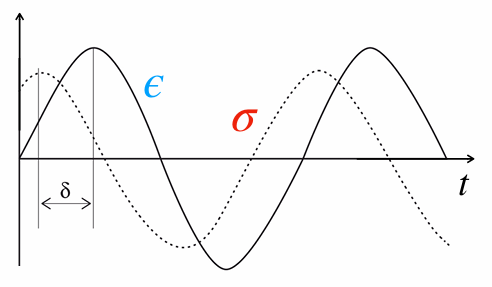
\includegraphics[width=0.5\linewidth]{fig/dynamic_test.png}
    \caption{Dynamic test.}
    \label{fig:dynamic_test}
\end{figure}

\noindent
Grazie a un creep test ideale è possibile caratterizzare i materiali secondo la loro natura reologica.\\

\noindent
Su tempi scala lunghi posso definire un materiale solido se, dopo una deformazione iniziale, mantiene la stessa forma; uno che fluisce indefinitamente invece è considerato un fluido.\\
Al contrario, a tempi scala più corti definisco altri comportamenti, come quello elastico e viscoelastico:
se lo strain aumenta linearmente con lo stress, il materiale è \textit{linearmente elastico}, 
mentre se è lo strain rate ad aumentare linearmente, il materiale è \textit{viscoso}, secondo la descrizione di Newton. 
Una combinazione dei due comportamenti caratterizza un corpo viscoelastico.

\subsection{\textcolor{colore7}{Comportamento elastico (corpo di Hooke)}}

L'estensione è proporzionale alla forza: \textit{Ut tensio, sic vis} (legge di Hooke, 1678).
Si tratta del comportamento reologico ideale noto come elasticità, tipicamente mostrato dai materiali cristallini a bassa temperatura e pressione.
Questo comportamento è definito da una deformazione istantanea all'applicazione del carico e da un recupero altrettanto immediato e totale una volta rimosso.
L'\textit{analogo meccanico} è una molla.\\

\noindent
\textbf{Legge di Hooke per i corpi elastici}: 
\begin{itemize}
    \item $\sigma = E \varepsilon$ (legge 1D, $E$ è una generica costante elastica);
    \item $\sigma_{ij} = C_{ijkl}\varepsilon_{kl}$ (legge in forma tensoriale);
    \item $\sigma_{ij} = 2\mu \varepsilon_{ij} + \lambda \varepsilon_{kk}\delta_{ij}$ (legge per corpi isotropi con $\mu$ e $\lambda$ costanti di Lamé).
\end{itemize}

\noindent \textbf{Creep test per un corpo elastico}: $\sigma = \sigma_0 H(t) \Longrightarrow \varepsilon = \frac{\sigma_0}{E}$.

\noindent \textbf{Relaxation test per un corpo elastico}: $\varepsilon = \varepsilon_0 H(t) \Longrightarrow\sigma = E \varepsilon_0 = cost.$\\

\noindent
Il comportamento elastico è valido esclusivamente al di sotto di una sollecitazione di soglia, detta \textit{limite elastico}.
Superata questa soglia, il materiale devia dalla linearità; per cui questa legge non spiega tutta la reologia.
La "costante" di proporzionalità $E$ (modulo di Young) in realtà aumenta con la pressione e diminuisce con la temperatura.
Il corpo elastico non subisce rilassamento.\\

\noindent
La litosfera superiore può essere modellata come un corpo elastico per carichi superficiali con durata dell'ordine di milioni di anni, sebbene la sua risposta reale sia viscoelastica.
Al contrario, tutta la Terra si comporta elasticamente (con imperfezioni) per carichi di breve durata (dai secondi alle ore),
il che rende la sismologia adatta ad un'analisi di tipo elastico.\\
A partire dalla sismologia è stato sviluppato il \textbf{modello PREM} (Preliminary Reference Earth Model), che lega la velocità delle onde s e p allo strato del Pianeta.

\begin{figure}[htb]
    \centering
    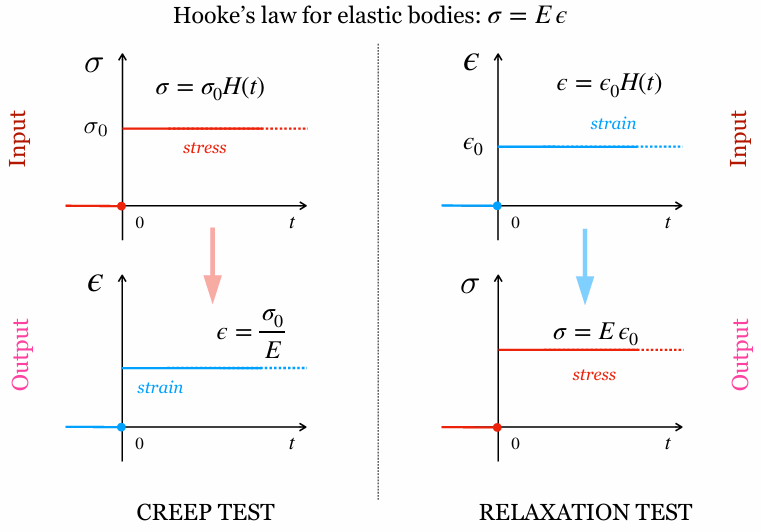
\includegraphics[width=0.7\linewidth]{fig/elastic_tests.png}
    \caption{Test meccanici ideali per un corpo elastico.}
    \label{fig:elastic_tests}
\end{figure}

\subsection{\textcolor{colore7}{Comportamento fluido (corpo di Newton)}}

All'estremo opposto dello spettro reologico rispetto ai solidi elastici si collocano i fluidi,
ovvero corpi che fluiscono in modo costante (\textit{steady-state flow}) se sottoposti a uno stress costante,
mostrando una deformazione che cambia continuamente nel tempo sotto qualsiasi carico, per quanto piccolo.\\
Il loro stato cinematico è descritto dal tensore del tasso di deformazione (\textit{strain rate tensor})
e il parametro caratteristico del materiale è la viscosità.
Su scale temporali geologiche, anche il mantello terrestre si comporta come un fluido.\\
In geodinamica, le due classi di fluidi più importanti sono i corpi newtoniani, in cui il tasso di deformazione è linearmente proporzionale allo stress,
e i corpi non newtoniani, in cui il tasso di deformazione è proporzionale allo stress elevato a una potenza $n$ (con $n > 1$).\\

\noindent
L'\textit{analogo meccanico} è uno stantuffo, che mostra un comportamento viscoso in cui la risposta dipende dal tempo:

\begin{equation}
    F = -k_v \frac{dx}{dt}
\end{equation}

\noindent
dove $k_v$ è la costante di dissipazione. Lo stress è proporzionale allo strain rate, vale cioè la \textbf{legge di Newton per i corpi fluidi}: $\sigma = \eta \dot{\varepsilon}$.\\

\begin{figure}[h!]
    \centering
    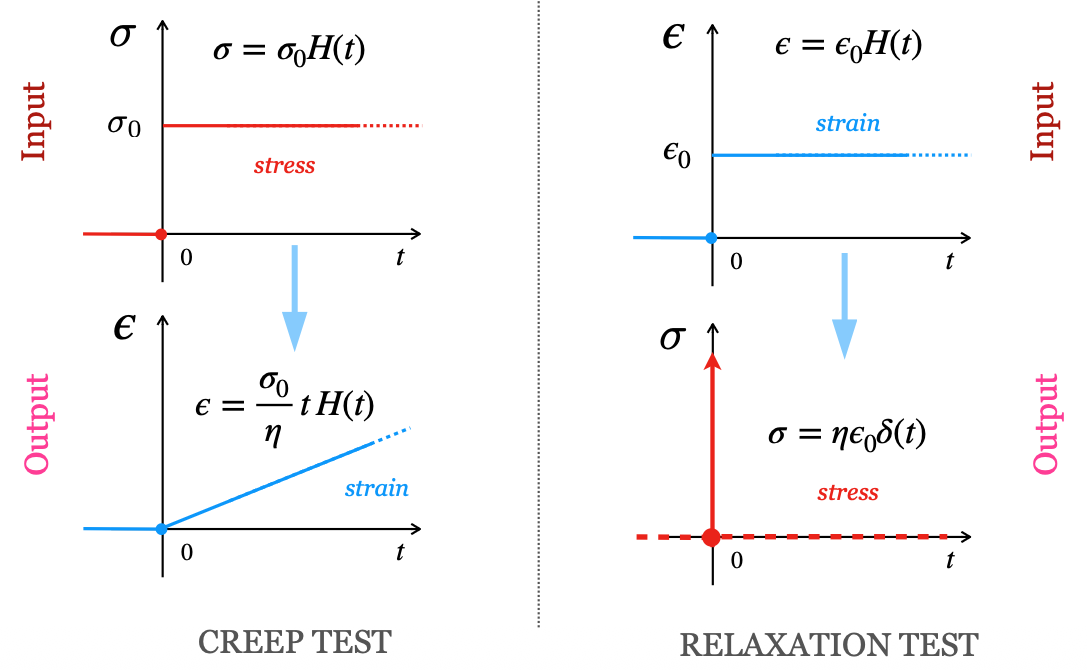
\includegraphics[width=0.7\linewidth]{fig/newton_tests.png}
    \caption{Test meccanici ideali per un corpo fluido.}
\end{figure}

\noindent
\textbf{Creep test per un corpo fluido}: $\sigma = \sigma_0 H(t) \Longrightarrow \varepsilon = \frac{\sigma_0}{\eta} t H(t)$.

\noindent
\textbf{Relaxation test per un corpo fluido}: $\varepsilon = \varepsilon_0 H(t) \Longrightarrow\sigma = \eta \varepsilon_0 \delta (t)$.\\

\noindent
dove $\eta = \sigma / \dot{\varepsilon}$ è la viscosità dinamica. Dimensionalmente:

\begin{equation}
    [\eta] = \frac{\text{stress}}{\text{strain rate}} = \text{pressione} \times \text{tempo} = \frac{FT}{L^2} = M L T^{-2} T L^{-2} = M L^{-1} T^{-1}
\end{equation}

\noindent
Nel SI $1 Pa \cdot s = 1 Pl$, con $Pl$ il \textit{Poiseuille}.\\

\noindent
Il \textit{Poise} $P$ è l'unità di misura della viscosità nel sistema cgs: $1 P = 1 g/cm/s = 0.1 Pl$.\\

\noindent
La viscosità cinematica è $\nu = \eta / \rho$. Dimensionalmente:

\begin{equation}
    [\nu] = \frac{\text{viscosità}}{\text{densità}} = \frac{M L^{-1} T^{-1}}{M L^{-3}} = \frac{L^2}{T}
\end{equation}

\noindent
La \textit{fluidità} è il reciproco della viscosità cinematica: $f = 1/\eta$.\\

\noindent
Grazie a un \textit{viscosimetro a piani paralleli} (flusso di Couvette), è possibile misurare lo shear in un fluido e da esso la viscosità dinamica:

\begin{figure}[htb]
    \centering
    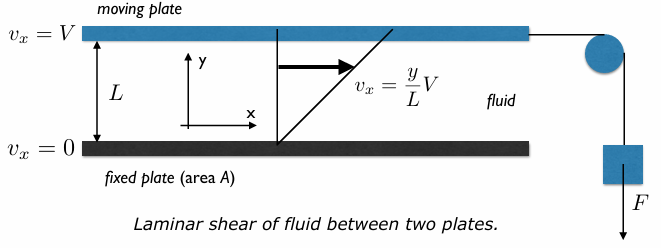
\includegraphics[width=0.7\linewidth]{fig/couvette.png}
    \caption{Viscosimetro di Couvette.}
    \label{fig:couvette}
\end{figure}

\begin{equation}
    \eta = \frac{L F}{A V}
\end{equation}

\noindent
Spesso la viscosità dinamica decade esponenzialmente con la temperatura.
Sia $Q$ l'energia di attivazione, $T$ la temperatura, $R$ la costante dei gas e $A$ una costante generica:

\begin{equation}
    \eta = A \cdot e^{\frac{Q}{RT}}
\end{equation}

\noindent
Si distinguono fluidi Newtoniani e non Newtoniani.
Nei primi la viscosità non dipende dallo stress (gas e molti liquidi), mentre nei secondi non vale la legge di Newton.
Si hanno perciò fluidi non Newtoniani:

\begin{itemize}
    \item \textit{shear-thickening}: la viscosità aumenta con lo strain rate;
    \item \textit{shear-thinning}: la viscosità diminuisce con lo strain rate;
    \item \textit{plastici di Bingham}: si comportano da solidi fino a un valore critico di stress, poi diventano dei fluidi viscosi: $\sigma = \eta \dot{\varepsilon} + cost.$
\end{itemize}

\noindent
Si può generalizzare la legge di Newton a più dimensioni:

\begin{itemize}
    \item $\sigma_{ij} = -p\delta_{ij} + C'_{ijkl} \dot{\varepsilon}_{kl}$ (forma tensoriale, dove $p$ è la pressione termodinamica e $C'_{ijkl}$ è il tensore dei parametri viscosi);
    \item $\sigma_{ij} = -p\delta_{ij} + \lambda' \dot{\theta} \delta_{ij} + 2\eta \dot{\varepsilon}_{ij}$ (legge per fluidi isotropi, dove $\theta = \dot{\varepsilon}_{kk}$ e $\lambda^\prime$ e $\eta$ sono parametri materiali). 
\end{itemize}

\noindent
L'isostasia glaciale e la convezione del mantello (che ha viscosità $\approx 10^{25}$ volte maggiore dell'acqua) si possono descrivere grazie a queste equazioni.

\newpage

\section{\textcolor{colore7}{Reologia II}}

\subsection{\textcolor{colore7}{Effetti temporali}}

In base alle condizioni esterne e alla durata del carico, le stesse rocce possono comportarsi in modi diversi e assumere comportamenti reologici opposti.
La risposta reologica dipende infatti da parametri sia intrinseci (proprietà del materiale) sia estrinseci (condizioni ambientali).\\

\noindent
Nella litosfera superiore, a basse temperature e pressioni, il comportamento è prevalentemente elastico, anche se sottoposto a carichi di lunga durata.
Al contrario, nel guscio della Terra (ad alte temperature e pressioni), la scala temporale del processo diventa rilevante:
il materiale risponde ancora in modo elastico se il carico è di breve durata, ma si comporta come un fluido (newtoniano o non newtoniano) se sottoposto a carichi di lunga durata.

Tra l'elasticità perfetta e il flusso stazionario si inserisce un comportamento intermedio, in cui la deformazione dipende dal tempo e il tasso di deformazione (\textit{strain rate}) a stress costante è una funzione decrescente con il tempo.

\begin{figure}[H]
    \centering
    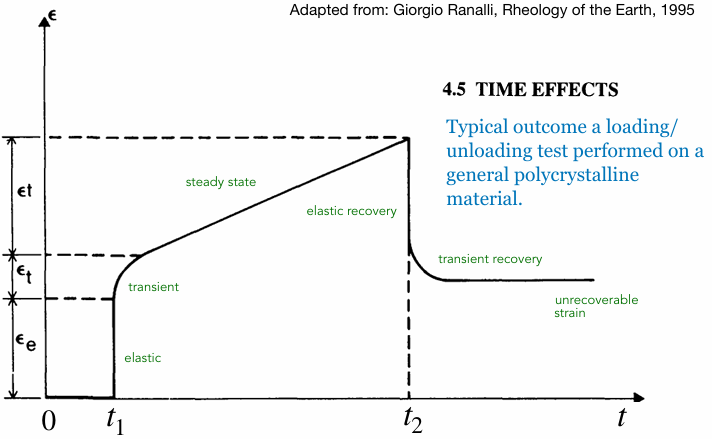
\includegraphics[width=0.7\linewidth]{fig/time_effects.png}
    \caption{Deformazione dipendente dal tempo sotto stress costante.}
    \label{fig:time_effects}
\end{figure}

\noindent
Per un carico applicato al tempo $t = t_1$ tipicamente si distinguono le seguenti fasi:

\begin{enumerate}
    \item \textbf{deformazione elastica istantanea} $\varepsilon_l$;
    \item \textbf{creep transiente} $\varepsilon_t$, in cui lo strain aumenta nel tempo con tasso decrescente;
    \item \textbf{creep stazionario} $\dot{\varepsilon}$, segue il creep transiente se le condizioni lo permettono
    (ad esempio la temperatura è sufficientemente alta) e se vi è sufficiente tempo; lo strain rate è costante;
    \item \textbf{recupero elastico istantaneo}, si verifica al tempo $t_2$ in cui il carico è rimosso.
    Si recupera lo strain elastico $\varepsilon_l$;
    \item \textbf{recupero transiente}, in cui su recupera lo strain transiente $\varepsilon_t$;
    \item \textbf{deformazione permanente}, acquisita durante la fase di creep stazionario; è permanente e non recuperabile.
\end{enumerate}

\noindent
Lo \textbf{strain creep totale} è dato da:

\begin{equation}
    \varepsilon(t) = \varepsilon_l + \varepsilon_t(t) + \dot{\varepsilon} t
\end{equation}

\noindent
dove la dipendenza temporale della funzione di creep transiente è variabile, per cui sono state proposte diverse leggi empiriche, il cui andamento è mostrato in Figura \ref{fig:transient_creep}:

\begin{itemize}
    \item \textit{legge esponenziale ritardata}: $\varepsilon_t (t) = A [1-exp(- \frac{t}{\tau})]$;
    \item \textit{equazione del creep di Andrade}: $\varepsilon_t (t) = \varepsilon_0 At^{1/\alpha}$;
    \item \textit{equazione di Scott-Blair}: $\varepsilon_t (t) = \frac{a}{\Gamma(1 + \nu)} * t^{\nu}$
    \item \textit{legge logaritmica}: $\varepsilon_t (t) = A log(1 + \alpha t)$;
    \item \textit{legge di Lomnitz modificata}: $\varepsilon_t (t) = \frac{\sigma}{\mu} \left(1 + \frac{q}{\alpha} [(1 + \alpha t)^\alpha -1] \right)$.
\end{itemize}

\begin{figure}[h!]
    \centering
    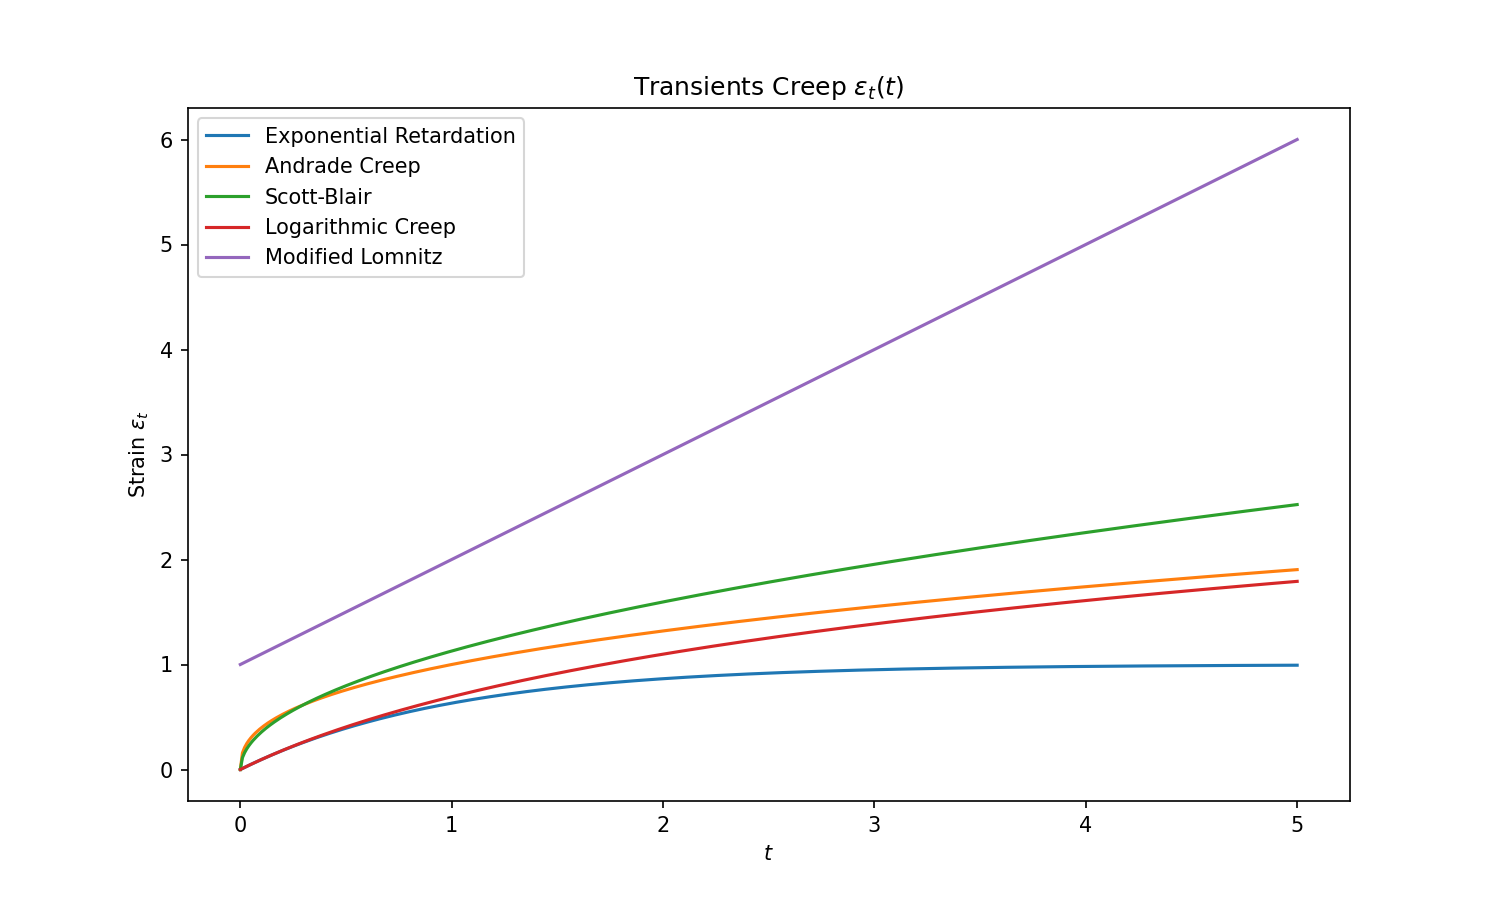
\includegraphics[width=0.7\linewidth]{fig/transient_creep.png}
    \caption{Funzioni di Creep transiente.}
    \label{fig:transient_creep}
\end{figure}

\noindent
Se la fase di creep stazionario non avviene e $\dot{\varepsilon}_t$ è una funzione decrescente con il tempo $t$, allora il materiale può essere
considerato essenzialmente elastico. 

\subsection{\textcolor{colore7}{Trasformate di Laplace}}

Sono strumenti matematici usati in ingegneria, che trovano utilizzo anche nella reologia.\\
La \textbf{trasformata di Laplace} di una funzione $f(t)$ è data da:

\begin{equation}
    \mathcal{L_-} \{f(t)\} \equiv \tilde{f}(s) = \int_{0^-}^\infty f(t) e^{-st} dt
\end{equation}

\noindent
dove $s = x + iy$ è la \textit{variabile complessa di Laplace}.
Con questa definizione il dominio di integrazione contiene l'eventuale singolarità in $t=0$.
Le trasformate di Laplace sono lineari:

\begin{equation}
    \mathcal{L_-} \{c f(t)\} = c\mathcal{L_-} \{f(t)\}
\end{equation}

\noindent
Le trasformate di Laplace sono omogenee e additive:

\begin{equation}
    \mathcal{L_-} \{f(t) + g(t)\} = \mathcal{L_-} \{f(t)\} + \mathcal{L_-} \{g(t)\}
\end{equation}

\noindent
La trasformata della derivata prima assume così la forma:

\begin{equation}
    \mathcal{L_-} \{f'(t)\} = s \tilde{f}(s) - f(0^-)
\end{equation}

\noindent
dove $f(0^-)$ è il \textit{valore pre-iniziale} di $f(t)$.\\

\noindent
Vale inoltre il \textit{teorema del valore iniziale}:

\begin{equation}
    \lim_{s \rightarrow{\infty}} s \tilde{f}(s) = f(0^+)
\end{equation}

\noindent
Date due funzioni $f(t)$ e $g(t)$, si può operare una \textbf{convoluzione temporale}:

\begin{equation}
    f(t) * g(t) = \int_{-\infty}^{+ \infty} f(t-t')g(t')dt' \mapsto \tilde{f}(s) \tilde{g}(s) 
\end{equation}

\noindent
Le trasformate mandano sistemi di equazioni differenziali in sistemi di equazioni lineari, in particolare, quelle di Laplace sono degli operatori integrali.

\subsection{\textcolor{colore7}{Comportamento viscoelastico (corpo di Maxwell)}}

Sono corpi viscoelastici che manifestano contemporaneamente proprietà tipiche dei corpi elastici e viscosi.
L'analogo meccanico è composto da un corpo di Hooke e uno di Newton in serie ($M = N - H$ nella notazione di Reiner).

\begin{figure}[h!]
    \centering
    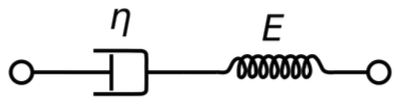
\includegraphics[width=0.4\linewidth]{fig/maxwell_body.png}
    \caption{Analogo meccanico del corpo viscoelastico.}
\end{figure}

\noindent
I due elementi sono soggetti allo stesso stress, ma a strain diversi.
Per linearità, applicando l'\textit{equazione costitutiva di Maxwell} vale allora:

\begin{equation}
    \dot{\varepsilon} = \dot{\varepsilon}_N + \dot{\varepsilon}_H = \frac{\sigma}{\eta} + \frac{\dot{\sigma}}{E}
\end{equation}

\noindent Dalla regola per le derivate, la trasformata di Laplace dell'equazione di Maxwell è data da:

\begin{equation}
    \mathcal{L}_- \{\dot \varepsilon(t) \} =  s \tilde{\varepsilon} - \varepsilon(0^-) = \mathcal{L}_- \{\dot \varepsilon_N(t) + \dot \varepsilon_H(t) \} = \frac{\tilde{\sigma}}{\eta} + \frac{1}{E} (s \tilde{\sigma} - \sigma (0^-))
\end{equation}

\noindent Considerando una condizione iniziale di equilibrio con $\sigma(0^-) = \varepsilon (0^-) = 0$, si risolve trovando:

\begin{equation}
    \tilde{\sigma} = \tilde{E}_M \tilde{\varepsilon}
\end{equation}

\noindent
dove 

\begin{equation}
    \tilde{E}_M = \frac{Es}{s + 1/\tau_M}
\end{equation}

\noindent
è il \textit{modulo complesso per la reologia di M}, mentre

\begin{equation}
    \tau_M = \eta/E
\end{equation}

\noindent
è il \textit{tempo di rilassamento di Maxwell}.\\

\noindent
Si noti l'analogia tra $\tilde{\sigma} = \tilde{E}_M \tilde{\varepsilon}$ e la legge di Hooke $\sigma = E \varepsilon$: è un'espressione del \textbf{principio di corrispondenza} della viscoelasticità lineare (\textit{la trasformata di Laplace dell'equazione reologica viscoelastica si ottiene dalle equazioni elastiche, cambiando i moduli elastici (come E) nei rispettivi moduli complessi ($\tilde{E}_M$) e cambiando $\sigma$ e $\eta$ in $\tilde{\sigma}$ e $\tilde{\eta}$}).
Tale principio risulta evidente applicando le trasformate di Laplace.\\

\noindent
\textbf{Creep test per un corpo viscoelastico}\\

\noindent
$\sigma (t) = \sigma_0 H(t) \Longrightarrow \tilde{\sigma} = \sigma_0 / s$.
Si ricava la \textbf{creep compliance} $\tilde J_M$, cioè lo strain per unità di stress in un esperimento di creep, che dipende dalla natura reologica del corpo:

\begin{equation}
    \frac{\tilde{\varepsilon}}{\sigma_0} = \frac{1}{s \tilde{E}_M} \equiv \tilde{J}_M
\end{equation}

\noindent Sostituendo, si ricava:

\begin{equation}
    \tilde{E}_M = \frac{Es}{s + 1/\tau_M} \Longrightarrow \tilde{J}_M = \frac{1}{Es} + \frac{1}{\eta s^2}
\end{equation}

\noindent Così la creep compliance di Maxwell nel dominio temporale è data dall'antitrasformata:

\begin{equation}
    J_M (t) = \frac{1}{E} H(t) + \frac{t}{\eta} \text{ , dove } t \ge 0
\end{equation}

\noindent
Il corpo maxwelliano sottoposto a stress costante mostra una risposta elastica istantanea,
seguita da un flusso con strain rate costante, senza una fase transiente intermedia.

\begin{figure}[htb]
    \centering
    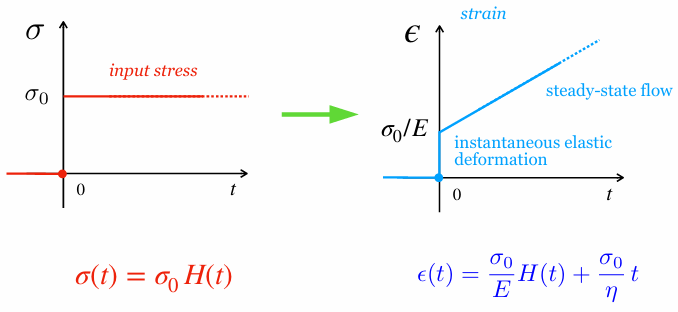
\includegraphics[width=0.7\linewidth]{fig/viscoelastic_creep.png}
    \caption{Creep test per un corpo con la reologia di Maxwell.}
    \label{fig:viscoelastic_creep}
\end{figure}

\noindent
\textbf{Relaxation test per un corpo viscoelastico}\\

\noindent
$\varepsilon (t) = \varepsilon_0 H(t) \Longrightarrow\tilde{\varepsilon} = \varepsilon_0/s$.
Si ricava il \textit{modulo di rilassamento}, cioè lo stress per unità di strain in un esperimento di rilassamento, che dipende dalla natura reologica del corpo:

\begin{equation}
    \frac{\tilde{\sigma}}{\varepsilon_0} = \frac{\tilde{E}_M}{s} \equiv \tilde{G}_M
\end{equation}

\noindent Sostituendo, si ricava:

\begin{equation}
    \tilde{E}_M = \frac{Es}{s + 1/\tau_M} \Longrightarrow \tilde{G}_M = \frac{E}{s + 1/\tau_M}
\end{equation}

\noindent Così il modulo di rilassamento di Maxwell nel dominio temporale è dato da:

\begin{equation}
    G_M(t) = Ee^{-t/\tau_M} \text{ , dove } t \ge 0
\end{equation}

\noindent Il corpo maxwelliano sottoposto a strain costante mostra uno stress che decade esponenzialmente nel tempo con costante di decadimento $\tau_M$.
Non tutti i sistemi viscoelastici si rilassano e non tutti quelli che lo fanno seguono necessariamente una legge esponenziale.

\begin{figure}
    \centering
    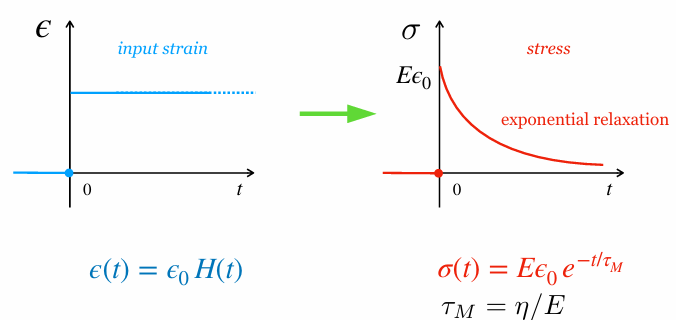
\includegraphics[width=0.7\linewidth]{fig/viscoelastic_relaxation.png}
    \caption{Relaxation test per un corpo con la reologia di Maxwell.}
    \label{fig:viscoelastic_relaxation}
\end{figure}

\subsection{\textcolor{colore7}{Considerazioni sulla reologia di corpi elastici, fluidi e viscoelastici}}

\begin{itemize}
    \item Corpo di Hooke: $\sigma = E \varepsilon \Longrightarrow \tilde{\sigma} = \tilde{E}_H \tilde{\varepsilon}$, dove $\tilde{E}_H = E$;
    \item Corpo di Newton: $\sigma = \eta \dot{\varepsilon} \Longrightarrow \tilde{\sigma} = \tilde{E}_N \tilde{\varepsilon}$, dove $\tilde{E}_N = \eta s$
\end{itemize}

\noindent Si noti che:

\begin{equation}
    \frac{1}{\tilde{E}_H} + \frac{1}{\tilde{E}_N} = \frac{1}{E} + \frac{1}{\eta s} = \frac{s + E/\eta}{Es} \equiv \frac{1}{\tilde{E}_M}
\end{equation}

\noindent
Cioè in un corpo di Maxwell, il reciproco del modulo complesso è pari alla somma dei reciproci dei moduli complessi del corpo di Hooke e di quello di Newton.\\

\noindent
Dato $\tilde{E}$, si hanno anche direttamente $\tilde{J} = 1/s \tilde{E}$ e $\tilde{G} = \tilde{E}/s$.
In ogni reologia lineare, vale:

\begin{equation}
    \tilde{J} \tilde{G} = \frac{1}{s^2}
\end{equation}

\noindent
Quindi, noto l'esito di un esperimento di creep $(\tilde J)$, i risultati dell'esperimento di rilassamento $(\tilde G)$ sono noti.\\

\noindent
Dall'antitrasformata di Laplace di questa relazione, si ottiene:

\begin{equation}
    \int_{-\infty}^{+\infty} J(t - t')G(t')dt' = \int_{-\infty}^{+\infty} J(t')G(t-t')dt' = t
\end{equation}

\noindent Per cui il problema di ricavare $G$ da $J$, o viceversa, è un problema di deconvoluzione.\\

\noindent
\textbf{Tempo di rilassamento di Maxwell della Terra}\\

\noindent
Il tempo di rilassamento di Maxwell della Terra è così dato dalla stima della viscosità derivante dagli studi del rimbalzo post-glaciale e dall'elasticità data dal modello PREM:

\begin{equation}
    \tau_M = \frac{\eta}{E} = \frac{\text{Bulk viscosity}}{\text{Bulk elasticity}} \approx \frac{10^{21 \div 22} Pa \cdot s}{10^{11} Pa} \approx 10^{10 \div 11} s \simeq 300 \div 3000 \text{anni}
\end{equation}

\noindent Perciò, assumendo che la reologia del mantello sia quella di un corpo di Maxwell, per tempi molto minori di $\tau_M$ la Terra si comporta in maniera elastica, mentre per tempi molto maggiori di $\tau_M$ si comporta in maniera viscoelastica.\\

\noindent
Si può così definire il \textbf{numero di Deborah} (dal nome della profetessa dell'Antico Testamento che disse "Dio è talmente grande che anche le montagne fluiscono sotto i suoi occhi").
È un numero adimensionale per caratterizzare quanto un materiale appaia fluido:

\begin{equation}
    De = \frac{\tau_{rel}}{\tau_{exp}} = \frac{\text{tempo di rilassamento}}{\text{tempo scala dell'esperimento}}
    \label{eq:deborah}
\end{equation}

\noindent
Quindi, minore il numero $De$, più il materiale appare fluido. Possiamo considerare tre esempi di processi per la Terra ($\tau_M \simeq 10^3$ anni):

\begin{itemize}
    \item Onde sismiche ($\tau_{exp} \simeq 1$ s): $De \sim \infty$ (comportamento elastico);
    \item Convezione del mantello ($\tau_{exp} \simeq 10^6$ anni): $De \sim 0$ (comportamento viscoso);
    \item Isostasia glaciale ($\tau_{exp} \simeq 10^3$ anni): $De \sim 1$ (comportamento viscoelastico).
\end{itemize}

\subsection{\textcolor{colore7}{Comportamento firmoviscoso (corpo di Kelvin-Voigt)}}

Un sistema formato da un corpo di Hooke e da uno di Newton in parallelo è detto \textbf{corpo di Kelvin-Voigt} e mostra un comportamento viscoelastico diverso da quello maxwelliano.
I due corpi sono sottoposti allo stesso strain ma a diverso stress.
L'analogo meccanico è composto da un corpo di Hooke e uno di Newton in parallelo. Si indica con $K = N|H$.

\begin{figure}[h!]
    \centering
    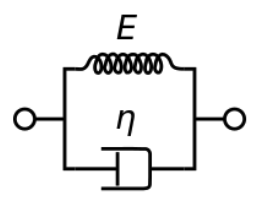
\includegraphics[width=0.2\linewidth]{fig/Kelvin_Voigt_body.png}
    \caption{Analogo meccanico del corpo firmoviscoso.}
\end{figure}

\noindent
Per linearità, lo stress totale è dato dalla somma espressa nell'\textit{equazione costitutiva di un corpo di Kelvin-Voigt}:

\begin{equation}
    \sigma = \sigma_N + \sigma_H = \eta \dot{\varepsilon} + E\varepsilon
\end{equation}

\noindent Dalla regola delle derivate delle trasformate di Laplace, si ha:

\begin{equation}
    \tilde{\sigma} = \eta (s\tilde{\varepsilon} - \varepsilon (0^-)) + E\tilde{\varepsilon} \Longrightarrow \tilde{\sigma}= \tilde{E}_K \tilde{\varepsilon} 
\end{equation}

\noindent
dove $\tilde{E}_K = \eta \left( s + \frac{1}{\tau_K}\right)$ è il \textit{modulo complesso della reologia di Kelvin-Voigt}.\\

\noindent Il \textit{tempo di ritardo} o \textit{tempo di rilassamento di Kelvin} è dato da $\tau_K = \eta/E$.
Vale il principio di corrispondenza della viscoelasticità lineare, come nel caso del corpo maxwelliano; inoltre, vale la somma dei moduli $\tilde{E}_K = \tilde{E}_N + \tilde{E}_H$.\\

\noindent
\textbf{Creep test per un corpo di Kelvin-Voigt}\\

\noindent
$\sigma(t) = \sigma_0 H(t) \Longrightarrow \tilde{\sigma} = \sigma_0 / s$.
La creep compliance del corpo di Kelvin-Voigt è data da:

\begin{equation}
    \frac{\tilde{\varepsilon}}{\sigma_0} = \frac{1}{s \tilde{E}_K} = \tilde{J}_K
\end{equation}

\noindent Sostituendo, si ha:

\begin{equation}
    \tilde{E}_K = \eta \left( s + \frac{1}{\tau_K} \right) \Longrightarrow \tilde{J}_K = \frac{1}{\eta s} \left( \frac{1}{s + 1/\tau_K} \right)
\end{equation}

\noindent Per ottenere la creep compliance nel dominio temporale, è necessario applicare il teorema di convoluzione al prodotto di due trasformate di Laplace.

\begin{equation}
    J_K(t) = \frac{1}{E} \left( 1 - e^{-t/\tau_K} \right)
\end{equation}

\noindent Si ottiene un'esponenziale ritardata, in grado di descrivere una reologia transiente:
il corpo non ha una risposta elastica istantanea, il flusso quindi avviene con uno strain rate variabile. Per tempi $t \rightarrow \infty$ si raggiunge uno strain costante.

\begin{figure}[H]
    \centering
    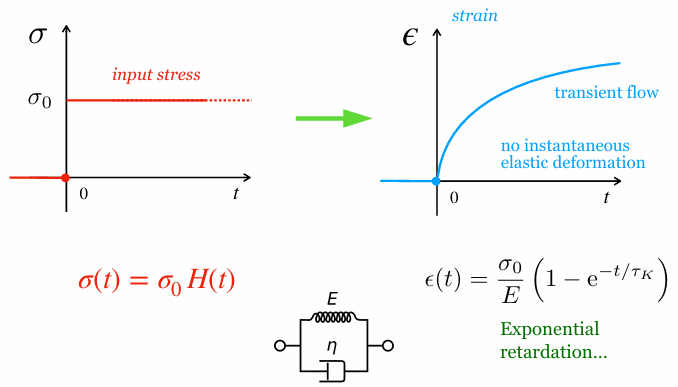
\includegraphics[width=0.7\linewidth]{fig/kelvin_creep.png}
    \caption{Creep test per un corpo di Kelvin-Voigt.}
    \label{fig:kelvin_creep}
\end{figure}

\noindent
\textbf{Relaxation test per un corpo di Kelvin-Voigt}\\

\noindent
$\varepsilon (t) = \varepsilon_0 H(t) \Longrightarrow \tilde{\varepsilon} = \varepsilon_0/s$.
Si ottiene un modulo di rilassamento, cioè il rapporto tra lo stress e lo strain in un esperimento di rilassamento, dato da:

\begin{equation}
    \frac{\tilde{\sigma}}{\varepsilon_0} = \frac{\tilde{E}_K}{s} \equiv \tilde{G}_K
\end{equation}

\noindent Sostituendo, si ha:

\begin{equation}
    \tilde{E}_K = \eta \left( s + \frac{1}{\tau_K} \right) \text{ , dove } \tilde{G}_K = \eta + \frac{E}{s}
\end{equation}

\noindent Si ricava così il modulo di rilassamento di un corpo di Kelvin-Voigt nel dominio temporale:

\begin{equation}
    G_K (t) = \eta \delta (t) + EH(t) \text{ , } t \ge 0
\end{equation}

\noindent
Cioè, per un corpo di Kelvin-Voigt soggetto a strain costante lo stress non decade nel tempo.

\begin{figure}[htb]
    \centering
    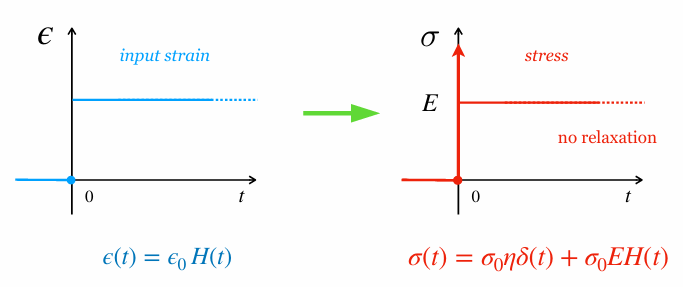
\includegraphics[width=0.5\linewidth]{fig/kelvin_relaxation.png}
    \caption{Relaxation test per un corpo di Kelvin-Voigt.}
    \label{fig:kelvin_relaxation}
\end{figure}

\subsection{\textcolor{colore7}{Proprietà dei modelli di H, N, M e K}}

Si riassumono il modulo effettivo, la creep compliance, il modulo di rilassamento e la viscosità effettiva per i modelli di Hooke, Newton, Maxwell e Kelvin-Voigt.

\begin{table}[htb]
\centering
\renewcommand{\arraystretch}{1.3}
\setlength{\tabcolsep}{8pt}
\begin{tabular}{|c|c|c|c|c|}
    \hline
    \textbf{Modello} & $\tilde{E}(s)$ & $J(t)$ & $G(t)$ & $\eta_{eff}(t) = 1/\dot{J}$ \\
    \hline
    \rowcolor{colore7!40}
    Hooke & $E$ & $1/E$ & $E$ & $\infty$ \\
    \hline
    \rowcolor{colore2!40}
    Newton & $\eta s$ & $t/\eta$ & $\eta \delta(t)$ & $\eta$ \\
    \hline
    \rowcolor{colore4!40}
    Maxwell & $\frac{Es}{s + E/\eta}$ & $\frac{H(t)}{E} + \frac{t}{\eta}$ & $E e^{-t/\tau_M}$ & $\eta$ \\
    \hline
    \rowcolor{colore5!40}
    Kelvin-Voigt & $\eta s + E$ & $\frac{1}{E} (1 - e^{-t/\tau_K})$ & $\eta \delta (t) + EH (t)$ & $\eta e^{t/\tau_K}$ \\
    \hline
\end{tabular}
\end{table}

\subsection{\textcolor{colore7}{Loading/unloading test per i modelli di H, N, M e K}}

Si consideri un esperimento di carico e scarico, per cui si applica uno stress dato da

\begin{equation}
    \sigma_{LU} (t) = \sigma_0 [H(t) - H(t-T)]    
\end{equation}

\noindent
dove $T>0$. Quindi:

\begin{itemize}
    \item un corpo di Hooke non mostra alcuna viscosità e c'è un recupero totale dello strain iniziale;
    \item un corpo di Newton non mostra elaticità, non c'è recupero dello strain iniziale e c'è uno strain permanente e flusso stazionario fino a $t=T$;
    \item per un corpo di Maxwell c'è recupero dello strain elastico, strain permanente e flusso stazionario fino a $t=T$;
    \item per un corpo di Kelvin-Voigt si osserva l'elasticità ritardata.
\end{itemize}

\begin{table}[htb]
\renewcommand{\arraystretch}{1.3}
\setlength{\tabcolsep}{8pt}
\centering
\begin{tabular}{|c|c|}
    \hline
    \textbf{Modello} & \textbf{Strain} \\
    \hline
    \rowcolor{colore7!40}
    Hooke & $\varepsilon_{LU} (t) = \varepsilon_0 [H(t) - H(t-T)]$ \\
    \hline
    \rowcolor{colore2!40}
    Newton & $\varepsilon_{LU} (t) = \frac{\sigma_0}{E} [t - (t-T)H(t-T)]$ \\
    \hline
    \rowcolor{colore4!40}
    Maxwell & $\varepsilon_{LU} (t) = \frac{\sigma_0}{2\eta} [H(t) - H(t-T)] + \frac{\sigma_0}{2\eta} [t - (t-T) H(t-\tau)]$ \\
    \hline
    \rowcolor{colore5!40}
    Kelvin-Voigt & $\varepsilon_{LU} (t) = \frac{\sigma_0}{2\eta} \left[\left(1 - e^{-\mu t/\eta} \right) - \left( 1 - e^{-(- \mu(t-T)t/\eta} \right) H(t-T) \right] $ \\
    \hline
\end{tabular}
\end{table}

\subsection{\textcolor{colore7}{Dynamic test per i modelli di H, N, M e K}}

Si consideri un esperimento dinamico, per cui si applica uno strain oscillante dato da

\begin{equation}
    \sigma(t) = \sigma_d cos \omega t
\end{equation}

\noindent
dove $t \ge 0$, $\sigma_d > 0$ e $\omega = 2\pi/P$. Si osserva che:

\begin{itemize}
    \item nel corpo di Hooke strain e stress sono in fase;
    \item nel corpo di Newton lo strain è sfasato di $90^\circ$;
    \item nel corpo di Maxwell lo strain è sfasato di una fase $\varphi$, dove $tan \varphi = -E/\eta \omega$;
    \item nel corpo di Kelvin-Voigt lo strain è sfasato di una fase $\varphi$, dove $tan \varphi = -c/s$.
\end{itemize}

\begin{table}[h!]
\renewcommand{\arraystretch}{1.3}
\setlength{\tabcolsep}{8pt}
\centering
\begin{tabular}{|c|c|c|}
    \hline
    \textbf{Modello} & \textbf{Legge costitutiva} & \textbf{Stress} \\
    \hline
    \rowcolor{colore7!40}
    Hooke & $\sigma = E \varepsilon$ & $\frac{\varepsilon(t)}{\sigma_d} = \frac{1}{E} cos \omega t$ \\
    \hline
    \rowcolor{colore2!40}
    Newton & $\dot{\varepsilon} = \frac{\sigma}{\eta}$ & $\frac{\varepsilon(t)}{\sigma_d} = \frac{1}{\eta \omega} sin \omega t$ \\
    \hline
    \rowcolor{colore4!40}
    Maxwell & $\dot{\varepsilon} = \frac{\sigma}{\eta} + \frac{\dot{\sigma}}{E}$ & $\frac{\varepsilon(t)}{\sigma_d} = \frac{1}{E} \cdot cos \omega t + \frac{1}{\eta \omega} \cdot sin \omega t$ \\
    \hline
    \rowcolor{colore5!40}
    Kelvin-Voigt & $\sigma = \eta \dot{\varepsilon} + E \varepsilon$ & $\frac{\varepsilon(t)}{\sigma_d} = c \cdot cos \omega t + s \cdot sin \omega t$\\
    \hline
\end{tabular}
\end{table}

\subsection{\textcolor{colore7}{Modelli di Maxwell generalizzati}}

Per un generico materiale viscoelastico lineare, lo strain rate è una funzione lineare delle derivate dello stress, quindi:

\begin{equation}
    \dot{\varepsilon} = \mathcal{F}(\sigma, \dot{\sigma}, \ddot{\sigma}, \dots; p_1, p_2, \dots)
\end{equation}

\noindent
con $p_i$ parametri del materiale. Ghiaccio e olivina sono due esempi di materiali reologici non lineari.\\

\noindent
Esistono altri modelli ottenuti a partire da quelli fondamentali già affrontati.\\

\noindent
Il \textbf{modello generalizzato di Maxwell} è costituito da un numero qualunque di elementi di Maxwell collegati fra loro in parallelo e rappresenta la forma più generale possibile di un modello di viscoelasticità.

\begin{equation}
    \text{GM} = \text{M}_1 | \dots | \text{M}_n
\end{equation}

\noindent
con $n$ un intero o $n=\infty$.
Questo modello tiene conto del fatto che il tempo di rilassamento non avviene ad un singolo tempo.
Prevede una risposta iniziale elastica, un periodo di transizione ed una fase stazionaria.\\

\subsection{\textcolor{colore7}{Modello di Burgers}}

Il \textbf{modello di Burgers} ($M - KV$) mostra un comportamento iniziale elastico, seguito da un creep transiente e da uno smorzamento delle vibrazioni su scale temporali ridotte, mentre su quelle più lunghe tende a mostrare un comportamento viscoelastico lineare.
Si utilizza spesso per modellare la reologia del mantello.

\begin{figure}[h!]
    \centering
    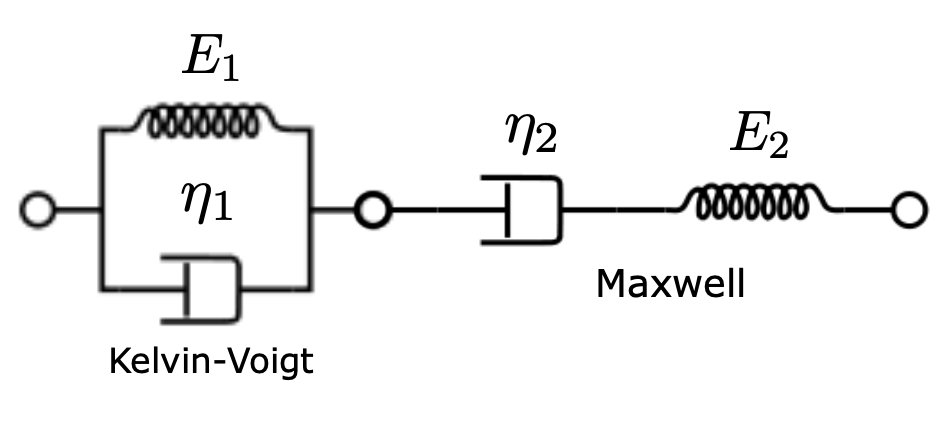
\includegraphics[width=0.5\linewidth]{fig/burgers_body.png}
    \caption{Analogo meccanico del modello di Burgers.}
\end{figure}

\noindent
\textbf{Creep test per il modello di Burgers}\\

\noindent
Le creep compliance si sommano, così che in totale si ha la somma di tre termini: la risposta elastica della molla $M$, la risposta transiente del corpo $KV$ e lo stato stazionario dello stantuffo $M$.

\begin{equation}
    J_B (t) = \frac{1}{E_2} H(t) + \frac{1}{E_1} \left( 1 - e^{-t/\tau_K} \right) + \frac{t}{\eta_2}
\end{equation}

\begin{figure}[h!]
    \centering
    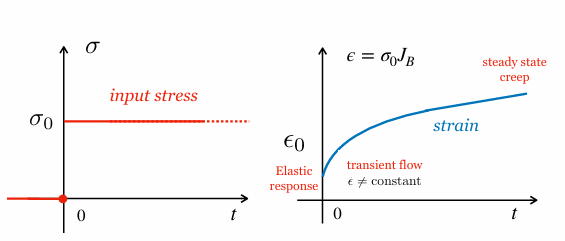
\includegraphics[width=0.7\linewidth]{fig/burgers_creep.png}
    \caption{Creep test per un corpo di Burgers.}
    \label{fig:burgers_creep}
\end{figure}

\noindent
\textbf{Relaxation test per il modello di Burgers}\\

\noindent
Il modulo di rilassamento determina uno spettro discreto di rilassamento, per cui si dice che il modello è \textit{biviscoso}.
Il modulo di rilassamento è dato da:

\begin{equation}
    G_B (t) = G_1 e^{- t/ \tau_1} + G_2 e^{- t/ \tau_2}
\end{equation}

\noindent
con $G_1$, $G_2$, $\tau_1$ e $\tau_2$ costanti positive determinate dai parametri del materiale $E_1$, $E_2$, $\eta_1$ e $\eta_2$.\\

\begin{figure}[h!]
    \centering
    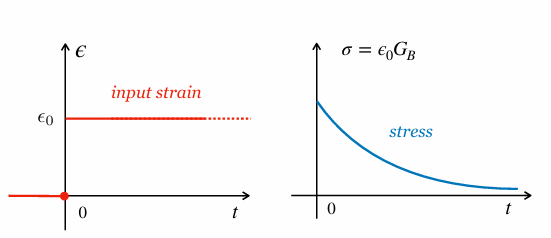
\includegraphics[width=0.65\linewidth]{fig/burgers_relaxation.png}
    \caption{Relaxation test per il modello di Burgers.}
    \label{fig:burgers_relaxation}
\end{figure}

\noindent
\textbf{Loading/unloading test per il modello di Burgers}\\

\noindent
Si ottiene la curva tipica del creep viscoelastico.

\begin{figure}[h!]
    \centering
    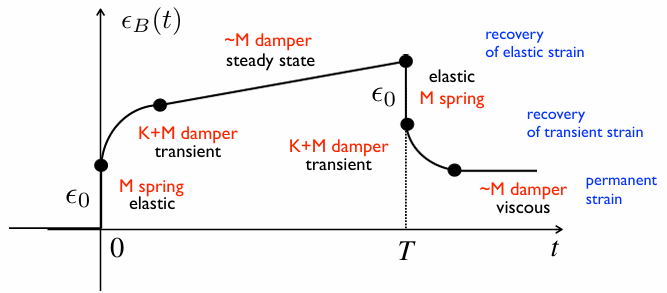
\includegraphics[width=0.7\linewidth]{fig/burgers_loading.png}
    \caption{Loading/unloading test per il modello di Burgers.}
    \label{fig:burgers_loading}
\end{figure}

\noindent
Si osservano tutte le fasi della deformazione di un corpo viscoelastico sottoposto a stress costante: la risposta elastica iniziale, quella transiente, lo stato stazionario, poi il recupero elastico, quello transiente e infine la deformazione non recuperabile.\\

\noindent
La reologia di Burgers ha tutte le proprietà mostrate dai quattro modelli reologici più semplici.

\begin{figure}[h!]
    \centering
    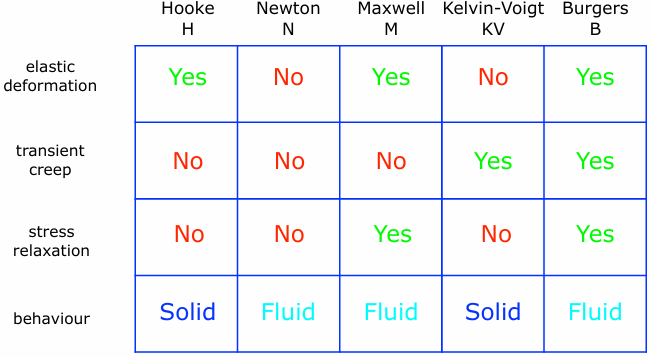
\includegraphics[width=0.55\linewidth]{fig/tabella_reologia.png}
    \caption{Tabella riassuntiva con le proprietà dei modelli analizzati.}
    \label{fig:tabella_reologia}
\end{figure}

\noindent Nel caso della \textbf{sequenza sismica}, si osservano tre fasi distinte: intersismica ($10 \div 1000$ anni), cosismica (secondi $\div$ minuti) e post-sismica (giorni $\div$ decenni).
La reologia di Burgers riesce a modellare bene le deformazioni post-sismiche.

\subsection{\textcolor{colore7}{Modello di Maxwell frazionario}}

Questo modello riesce a descrivere ancora meglio fenomeni quali le deformazioni post-sismiche,
sostituendo lo stantuffo Newtoniano nel corpo di Maxwell con uno \textit{stantuffo frazionario di Scott Blair}.

\begin{figure}[h!]
    \centering
    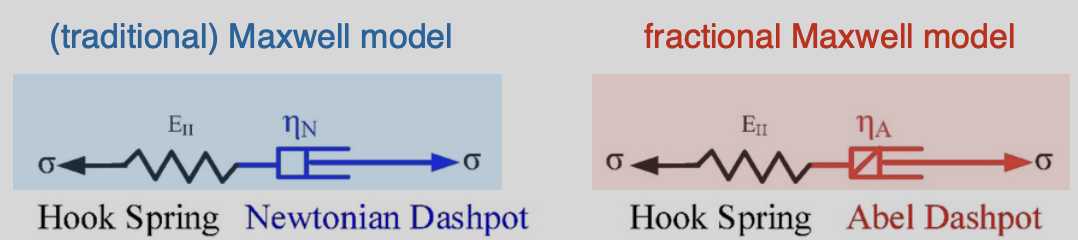
\includegraphics[width=0.6\linewidth]{fig/fractional_maxwell.png}
    \caption{Confronto tra modello di Maxwell tradizionale e frazionario.}
\end{figure}

\noindent
\textbf{Creep test per un modello di Maxwell frazionario}\\

\noindent
$\sigma(t) = \sigma_0 H(t)$, quindi la funzione di Creep è:

\begin{equation}
    J(t) = A + B t^\nu
\end{equation}

\noindent
dove $0<\nu\le1$.\\

\noindent
\textbf{Relaxation test per un modello di Maxwell frazionario}\\

\noindent
$\varepsilon (t) = \varepsilon_0 H(t)$, in questo caso, per il modulo di rilassamento è necessario ricorrere alla \textit{funzioni di Mittag-Leffler}, che generalizza il concetto di funzione $\Gamma$ considerando una derivata di ordine frazionario:

\begin{equation}
    E_\nu (z) = \sum_{n=0}^\infty \frac{z^n}{\Gamma(\nu n + 1)}
\end{equation}

\noindent
dove con $\nu = 1$ si recupera il modello di Maxwell classico. In questo modo il modulo di rilassamento è:

\begin{equation}
    G(t) = C E_\nu [-(t/\tau)^\nu]
\end{equation}

\noindent
Si hanno due incognite fondamentali per poter considerare il rimbalzo post-glaciale un creep test naturale della Terra: la storia del carico esercitato dai ghiacciai sulla superficie nel tempo e la reologia della Terra.

\newpage

\section{\textcolor{colore2}{Idrosfera}}

\subsection{\textcolor{colore2}{Introduzione e motivazione}}

Si studia il tasso di cambiamento del livello del mare per ragioni scientifiche e socioeconomiche, da alcuni decenni grazie anche all'altimetria satellitare, oltre ai mareografi.
Tra il 1993 e il 2003 si è osservato un innalzamento di $+2.8 \pm 0.4$ mm/anno, da confrontare con valori compresi fra 1 e 2 mm/anno dei decenni precedenti.
Il contributo principale è dato dall'espansione termica,
tuttavia, le stime sono ancora incerte per escludere i contributi di altre fonti, come lo scioglimento dei ghiacciai e del ghiaccio polare.
La distribuzione geografica di questo cambiamento non è uniforme a causa di tale effetto.\\

L'andamento fino al 1900 è dato da stime geologiche, poi sono arrivate le osservazioni mareografiche e l'altimetria satellitare negli anni Novanta.
L'andamento futuro è stimato empiricamente sulla base della temperatura o grazie a dei modelli di previsione.\\

\noindent
\textbf{Mareografo}\\

\noindent
Una barra graduata viene inserita in mare, spesso in un porto, così da misurare il \textit{livello marino relativo}, cioè rispetto alla Terra solida.
Si hanno perciò diverse contaminazioni dovute a vari fenomeni geologici.
Grazie ai circa 1500 mareografi presenti nel mondo, è stato possibile ricavare un trend a partire dal 1870 di $+1.8 \pm 0.2$ mm/anno.\\

\noindent
\textbf{Altimetro satellitare}\\

\noindent
A partire dal 1993 si può studiare l'altezza del geoide con grande precisione, ricavando un trend del \textit{livello marino assoluto} di $+3.2 \pm 0.4$ mm/anno.\\

\noindent
\textbf{Variazione del livello marino}\\

\begin{figure}[h!]
    \centering
    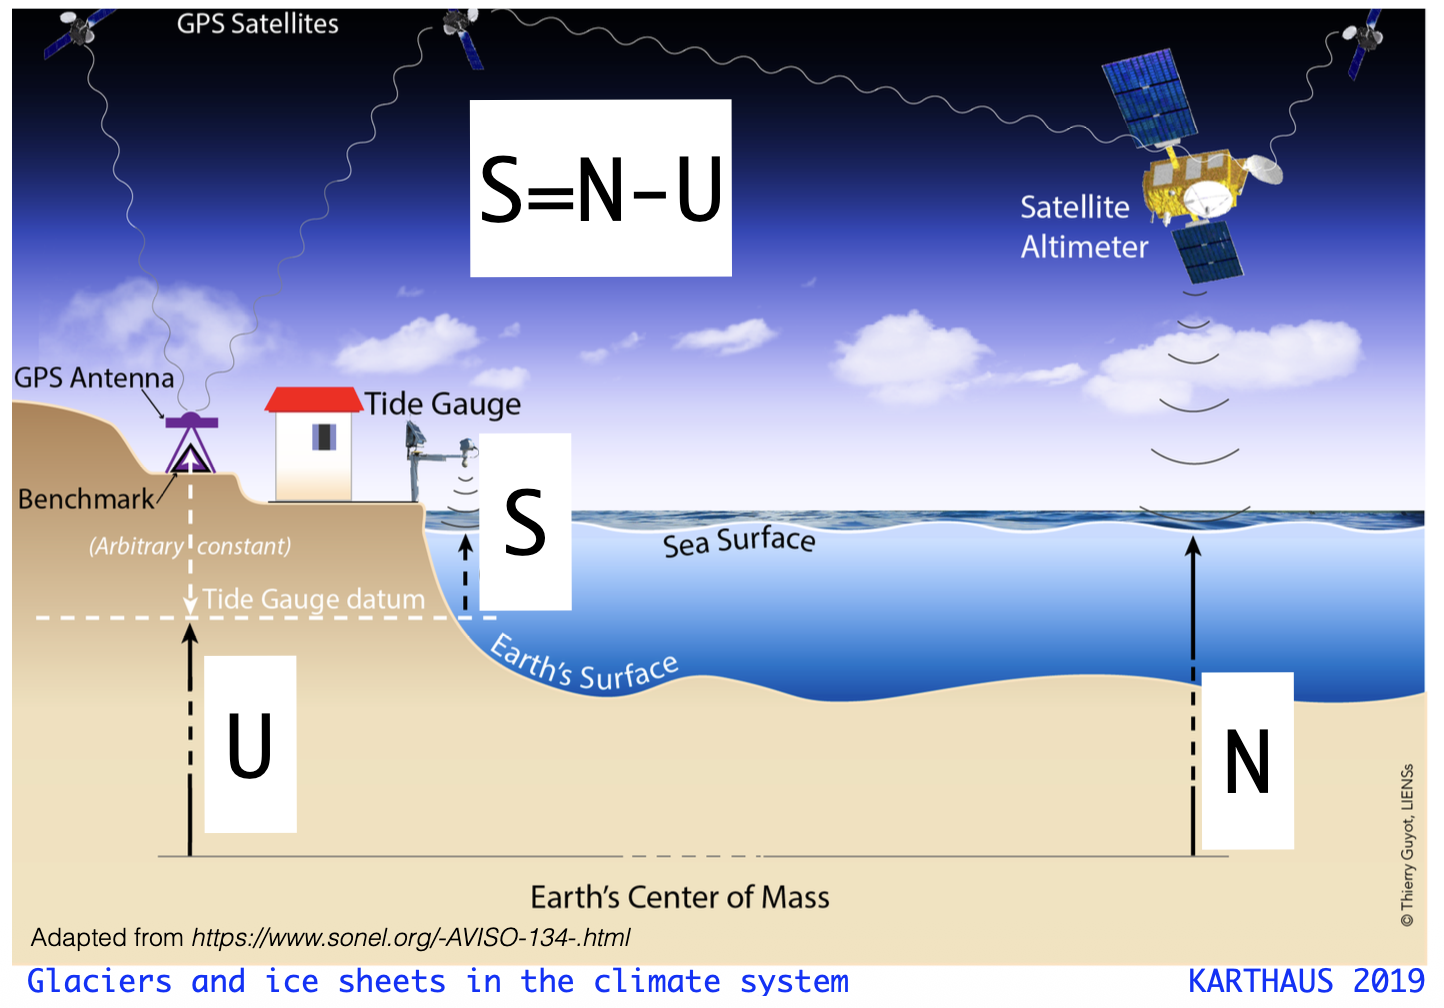
\includegraphics[width=0.5\linewidth]{fig/sea_level_eq.png}
    \caption{Equazione del livello marino.}
\end{figure}

\noindent
Si indica con $S$ il livello marino relativo, rispetto alla Terra solida, con $N$ quello assoluto, rispetto al centro di massa della Terra e con $U$ lo spostamento verticale.
Si ottiene una semplice equazione per il livello marino:
\begin{equation}
    S = N - U    
\end{equation}

\noindent
L'espansione termica è il termine attualmente dominante per l'innalzamento, poi c'è lo scioglimento di ghiacciai, Groenlandia e Antartide e l'aggiustamento glaceoisostatico.\\

\begin{figure}[h!]
    \centering
    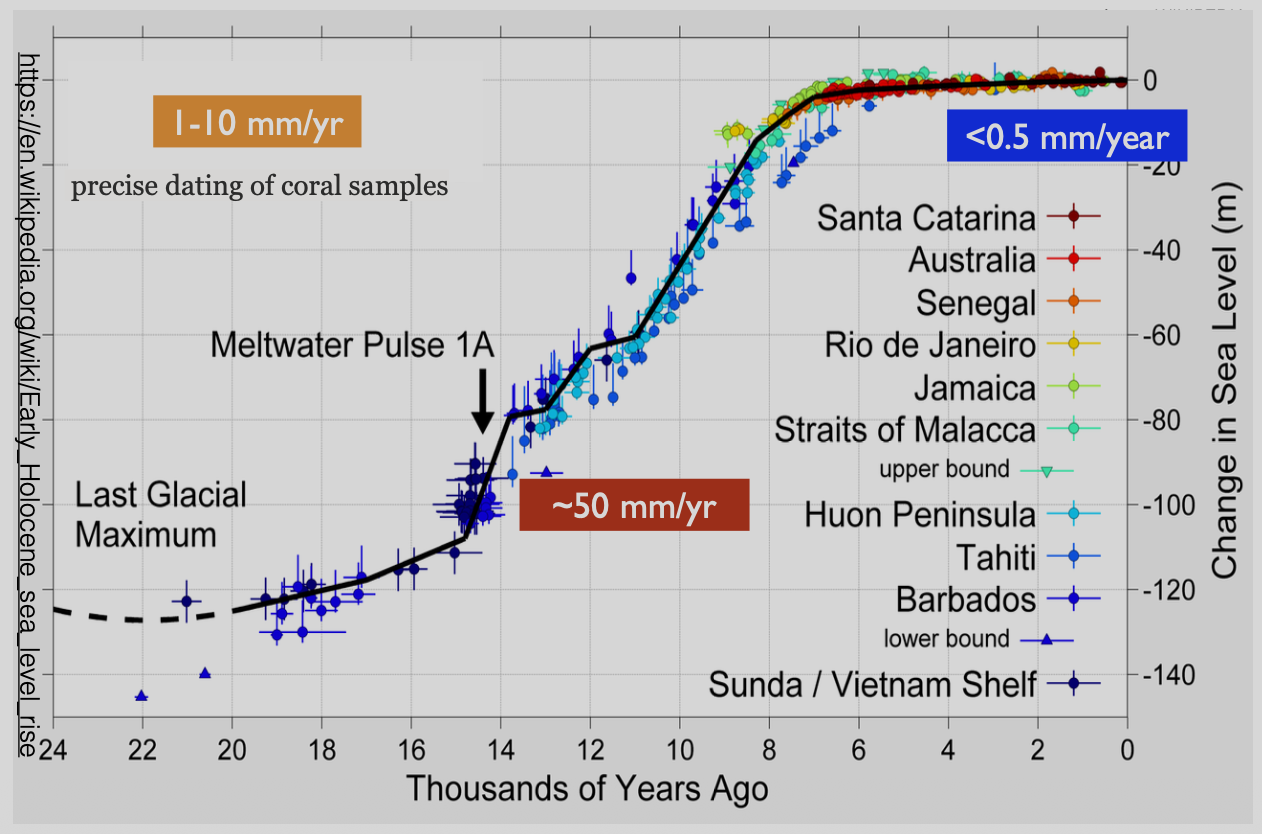
\includegraphics[width=0.5\linewidth]{fig/sea_level_21.png}
    \caption{Livello marino degli ultimi 21 mila anni.}
    \label{fig:sea_level}
\end{figure}

\noindent
Dall'ultimo massimo glaciale ($\approx$ 21'000 anni fa) fino a circa 6'000 anni fa, il livello del mare è aumentato di circa 130 m a causa della fusione delle masse glaciali (Figura \ref{fig:sea_level}).\\

\noindent
I cinque segnali vitali del pianeta, secondo la NASA, sono la concentrazione di $CO_2$, la temperatura globale, il minimo del ghiaccio marino artico, il ghiaccio terrestre e il livello del mare.

\subsection{\textcolor{colore2}{Registri individuali del livello marino}}

\subsubsection{\textcolor{colore2}{Piscine Romane}}

Le ville in riva al mare (come la Villa di Tiberio del II sec.) ospitavano delle piscine per l'itticoltura.
Grazie a queste si può misurare un aumento del livello marino relativo di $58 \pm 5$ cm, pesantemente influenzato dalla glaceoisostasia.

\subsubsection{\textcolor{colore2}{Terremoto di Messina del 28/12/1908}}

Un terremoto di magnitudo 7 causò un maremoto e circa 75'000 morti.
L'anomalia mareografica è stata misurata anche nel Tirreno a grande distanza.
Il mareografo di Messina così ha ricoperto il ruolo di sismografo a bassa frequenza, misurando uno spostamento elastico istantaneo di circa 50 cm e una risposta viscoelastica successiva, che potrebbe indicare un coinvolgimento di parte del mantello superiore.

\subsection{\textcolor{colore2}{Osservazioni strumentali dai registri globali}}

Si osserva un'oscillazione significativa con un periodo di circa 60 anni in quasi tutti i mareografi durante il XX sec., dovuta alle pulsazioni oceanografiche.
Questo rende impossibile trarre conclusioni su un trend di lungo periodo, permettendo solo stime sulla tendenza nel breve periodo.
Per questo motivo si richiede un registro di almeno 60 o 70 anni nei dati di un mareografo, il che ne esclude circa il 90\% (Figura \ref{fig:gauge_distribution}).\\

\begin{figure}[h!]
    \centering
    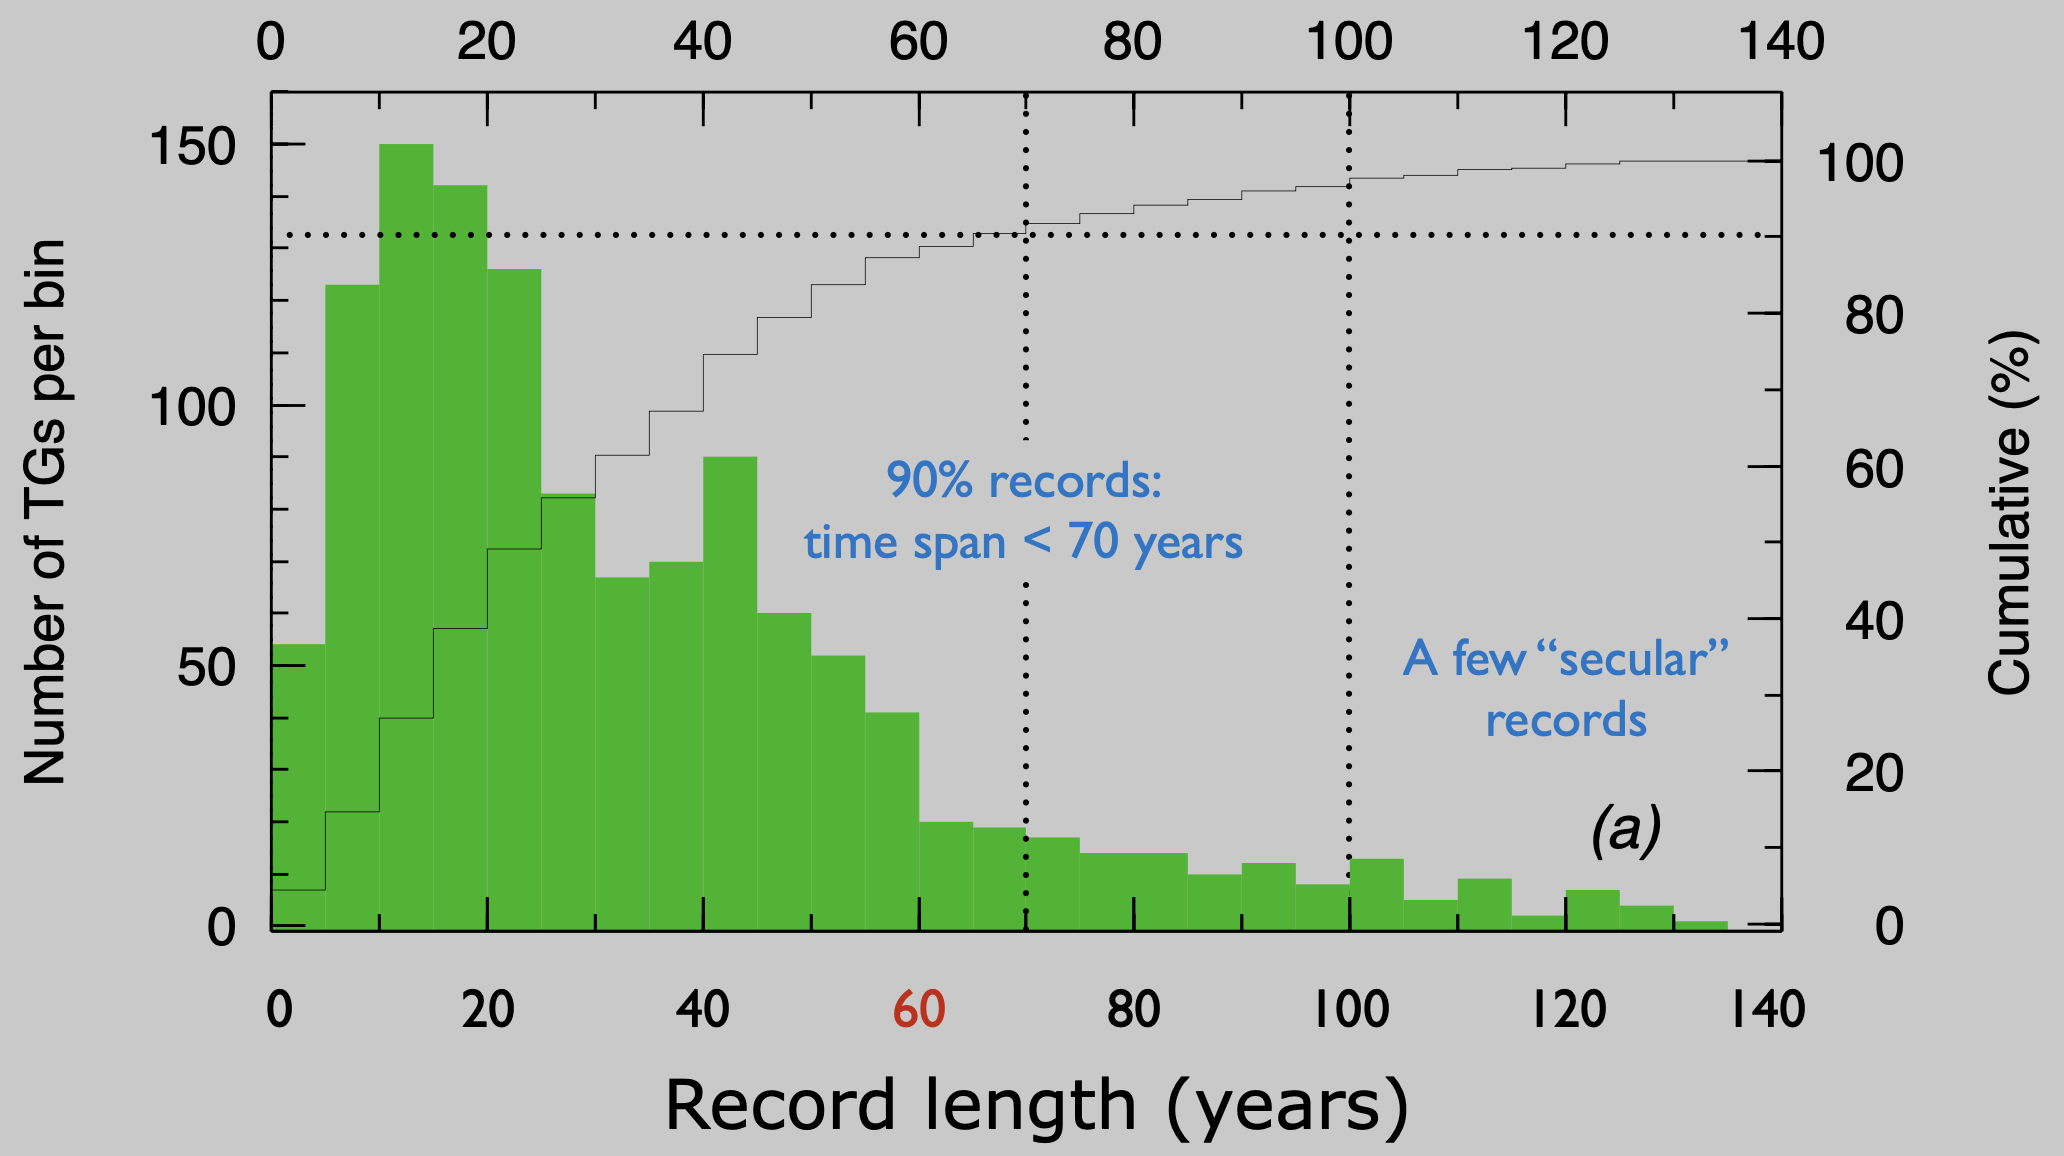
\includegraphics[width=0.5\linewidth]{fig/gauge_distribution.png}
    \caption{Distribuzione dei mareografi in funzione del periodo di attività.}
    \label{fig:gauge_distribution}
\end{figure}

\noindent
Un'altra limitazione è data dalla distribuzione non omogenea dei mareografi (Figura \ref{fig:gauge_spatial}) e dall'incompletezza dei loro dataset.

\begin{figure}[h!]
    \centering
    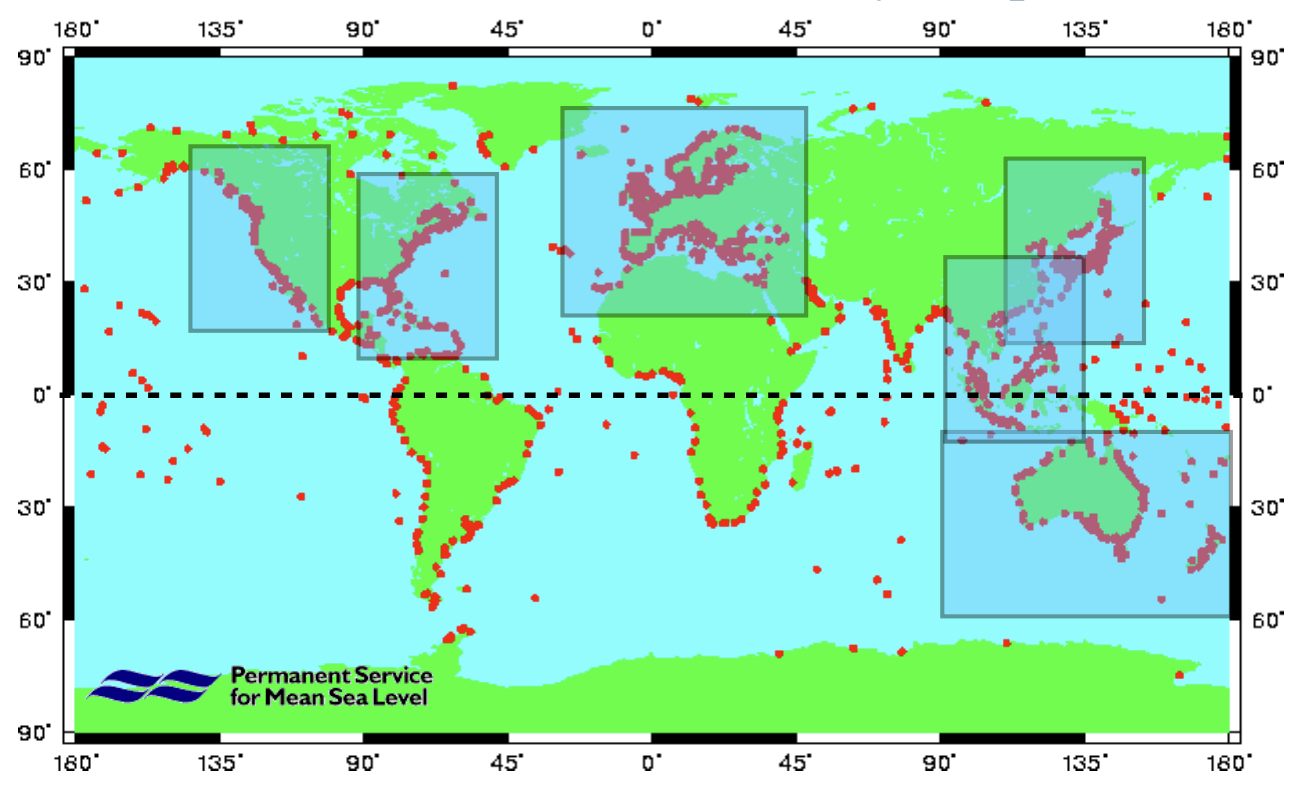
\includegraphics[width=0.55\linewidth]{fig/gauge_spatial.png}
    \caption{Distribuzione spaziale dei mareografi.}
    \label{fig:gauge_spatial}
\end{figure}

\noindent
Il \textit{Permanent Service for Mean Sea Level} (PSMSL) si occupa di standardizzare le misure.
L'approccio più usato è quello dell'\textit{ordinary least squares}, grazie al quale si ottiene, per esempio, un aumento di $1.5 \pm 0.2$ mm/anno a Trieste.\\

\noindent
Il \textit{best fit rate} per un numero $N_{tg}$ di mareografi dal database del PSMSL è così dato da:

\begin{equation}
    r_k = \frac{N_k^v \sum_j x_j y_j - \left(\sum_j x_j\right) \left(\sum_jy_j\right)}{N_k^v \left(\sum_j x_j^2 - \sum_j y_j^2 \right)}
    \label{eq:best_fit}
\end{equation}

\noindent
dove $k = 1,...,N_{tg}$ e:

\begin{itemize}
    \item $y_j$ è il livello del mare al tempo $x_j$ , con $j = 1,...,N_k^v$;
    \item $N_k^v$ è il numero di dati annuali validi nella serie temporale;
    \item $\sigma_k$ è l'incertezza del trend (95\% di confidenza).
\end{itemize}

\noindent
Quindi la variazione misurata dal mareografo è $\rho_k = r_k \pm \sigma_k$.\\

\noindent
A causa delle oscillazioni decennali, le serie temporali di durata maggiore di 60 anni tendono a mostrare variazioni molto più contenute e incertezze minori.
Alcuni mareografi misurano una diminuzione del livello marino a causa del rimbalzo glaceoisostatico.

\begin{figure}[h!]
    \centering
    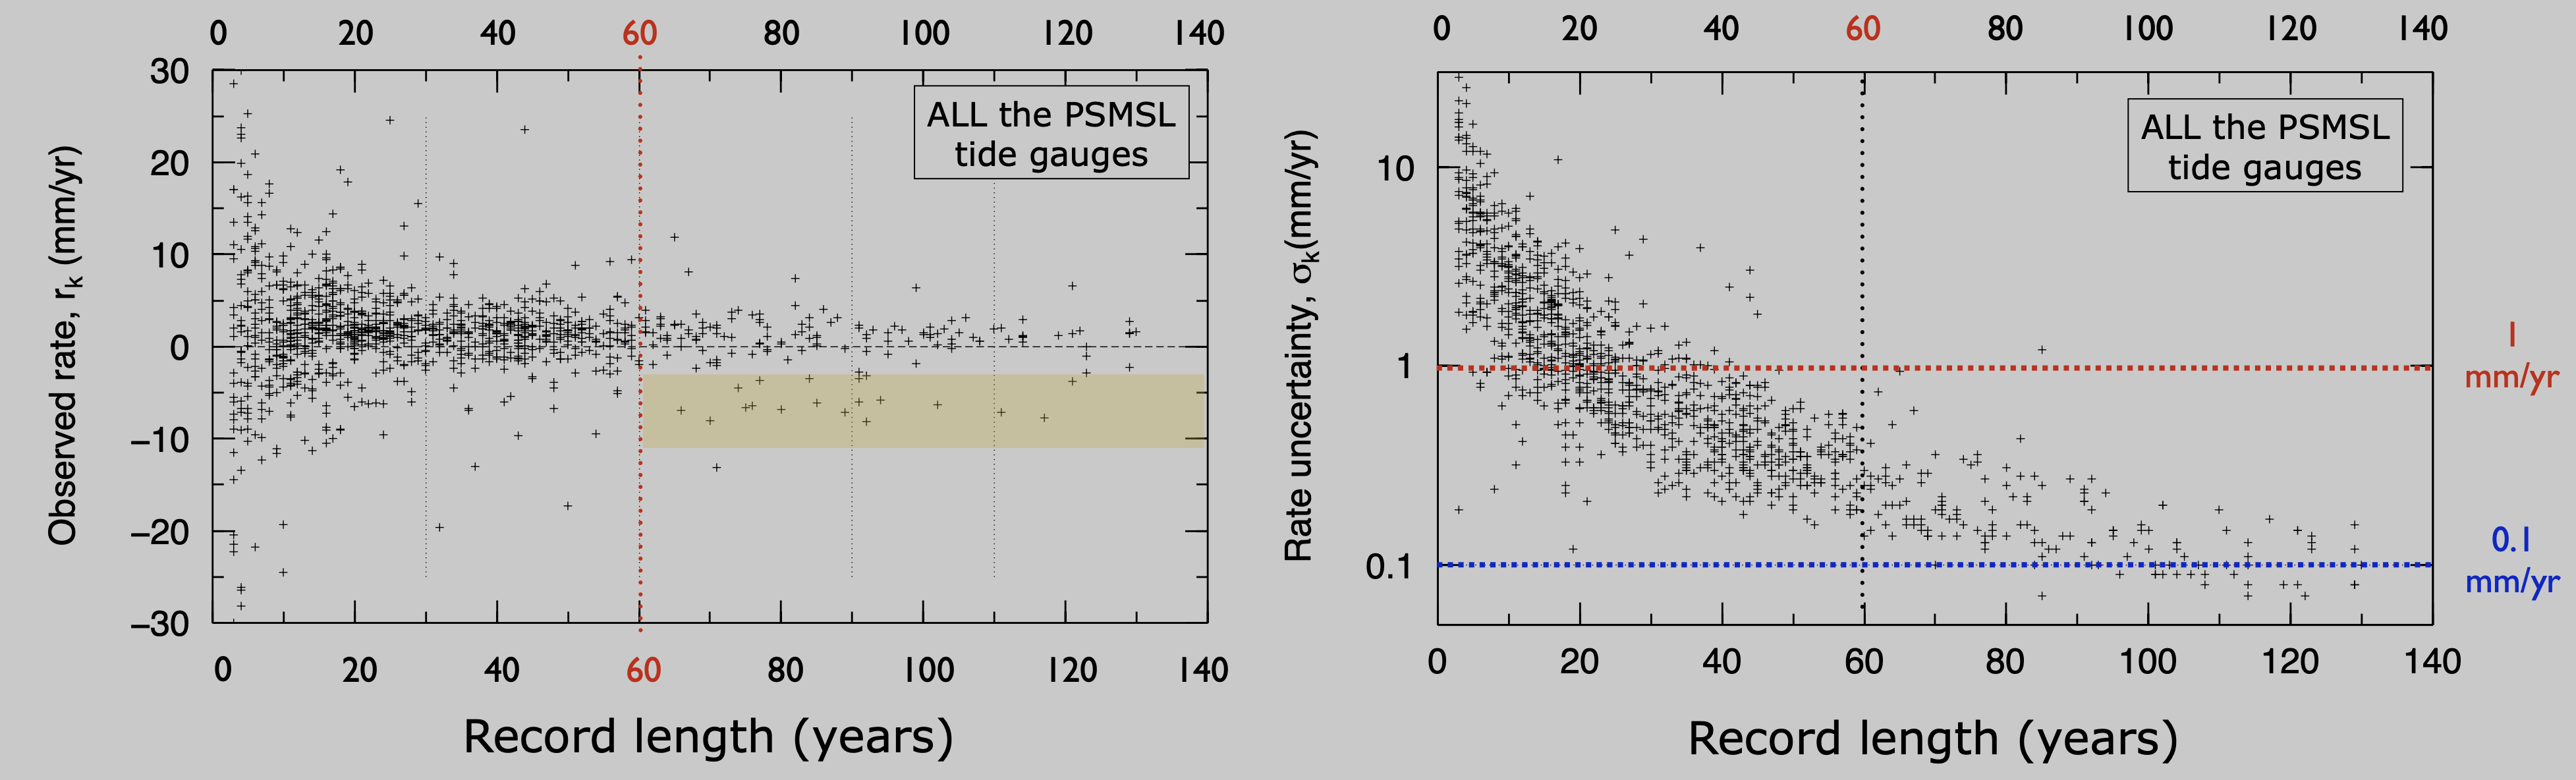
\includegraphics[width=1.0\linewidth]{fig/guage_rates.png}
    \caption{Tassi di variazione misurati dai mareografi e loro incertezze.}
\end{figure}

\subsection{\textcolor{colore2}{Problema della contaminazione glaceoisostatica}}

Un ulteriore fattore che impatta anche i record più lunghi è rappresentato dai segnali non oceanici.
A causa dello scioglimento dei ghiacciai, si misura un rimbalzo post-glaciale in corrispondenza delle regioni in cui erano presenti delle lenzuola glaciali.
Altri fattori che rendono la Terra solida instabile sono i terremoti, l'estrazione di acqua dal suolo, il deposito di materiali fluviali e la cementificazione.
A causa del maggiore carico che grava sugli oceani, anche la crosta oceanica sta subsidendo.\\

\noindent
Questi effetti contaminano i dati relativi al livello marino, come descritto dall'equazione del livello marino $S(\omega, t) = N - U$,
che si può risolvere con tecniche di tipo iterativo, partendo da soluzioni ragionevoli e ponendo approssimazioni più volte fino a convergere ad un valore.
Generalmente si parte considerando per $S$ il valore eustatico.\\

\noindent
L'equazione del livello marino introdotta da Farrell e Clark nel 1976 ha forma:

\begin{equation}
    S = \frac{\rho_i}{\gamma} G_s \otimes_i I +
        \frac{\rho_w}{\gamma} G_s \otimes_o S -
        \frac{m_i}{\rho_w A_o} -
        \frac{\rho_i}{\gamma} \overline{G_s \otimes_i I} +
        \frac{\rho_w}{\gamma} \overline{G_s \otimes_o S}
\end{equation}

\noindent
con:

\begin{itemize}
    \item $S$, variazione del livello del mare;
    \item $\rho_i$ e $\rho_w$, densità del ghiaccio e dell'acqua;
    \item $G_s$, funzione di Green per il livello del mare;
    \item $I$, variazione dello spessore del ghiaccio;
    \item $m_i$, variazione della massa del ghiaccio;
    \item $A_o$, area degli oceani;
    \item $\otimes_i$ e $\otimes_o$, convoluzioni 3D;
    \item $\overline{(\dots)}$, media dell'oceano.
\end{itemize}

\subsection{\textcolor{colore2}{Aumento del livello marino nell'ultimo secolo}}

Si riprende il \textit{best fit rate} (Equazione \ref{eq:best_fit}).
In letteratura, l'aumento globale del livello del mare si ottiene generalmente calcolando la media dei trend misurati dai mareografi:

\begin{equation}
    m=\frac{\sum_kr_k}{N_{tg}}
\end{equation}

\noindent
Questa media aritmetica è la miglior stima dell'\textbf{aumento medio globale del livello del mare} (GMSLR).\\

\noindent
L'incertezza sulle misure non è sempre disponibile, ma è fondamentale per calcolare la variazione del livello del mare medio globale.
La \textit{root mean square}:

\begin{equation}
    rms = \sqrt{\frac{\sum_k (r_k - m)^2}{N_{tg} - 1}}
\end{equation}

\noindent
rappresenta l'incertezza media dei singoli trend.
La \textit{standard deviation} della media:

\begin{equation}
    sdom=\frac{rms}{\sqrt{N_{tg}}}
\end{equation}

\noindent
rappresenta l'incertezza della stima $m$.\\

\noindent
Quindi, la GMSLR è data da:

\begin{equation}
    \mu = m \pm sdom
\end{equation}

\noindent
Nel 1941 Gutenberg fece una prima stima senza correzioni glaceoisostatiche ($1.1 \pm 0.8$ mm/anno).
In seguito altre stime non fornirono l'incertezza, fino a Peltier e Tushingham ($2.4 \pm 0.9$ mm/anno).
Pirazzoli nel 1986 ritenne impossibile calcolarlo per via dei troppi errori e del problema di mediare le incertezze.
In generale le stime non corrette per la glaceoisostasia restituiscono valori inferiori siccome molte misure sono fatte in zone vicine ai poli.\\

\noindent
Nel 1997 Douglas propose dei \textbf{criteri di selezione} per i mareografi:

\begin{enumerate}
    \item almeno 60 anni di dati;
    \item lontano dai confini delle placche tettoniche;
    \item completi almeno all'80\%;
    \item in accordo ragionevole (a basse frequenze) con i mareografi vicini;
    \item lontano da aree coperte di ghiacci durante l'ultimo massimo glaciale.
\end{enumerate}

\noindent
In questo modo restano solamente 23 mareografi (tutti in accordo, ma non necessariamente accurati), grazie ai quali si ricava un aumento, corretto per la glaceoisostasia, di $1.8 \pm 0.1$ mm/anno.
Diverse combinazioni di reologia e glaceoisostasia fittano le stesse osservazioni, per cui non si ha una soluzione univoca.

\newpage

\section{\textcolor{colore7}{Distribuzioni superficiali di massa}}

\subsection{\textcolor{colore7}{Motivazione}}

La superficie terrestre è sottoposta al carico della massa dell'atmosfera, degli oceani e dei continenti; questi possono variare nel tempo e causare una risposta elastica o viscoelastica, a seconda del numero di Deborah (Eq. \ref{eq:deborah}).
Terremoti, eruzioni vulcaniche, moti mareali e frane possono variare il carico sulla superficie.\\

\noindent
Il \textbf{modello di Boussinesq} prevede una Terra piatta ed elastica, con modulo di shear $\mu$ e rapporto di Poisson $\nu$ costanti, su cui viene esercitato un carico.
La deformazione avviene sia in orizzontalmente in direzione radiale:

\begin{equation}
    u_r = \frac{P}{4\pi \mu R} \left[ \frac{rz}{R} - \frac{(1-2\nu)r}{R+z} \right]
\end{equation}

\noindent
che in verticalmente:

\begin{equation}
    u_z = \frac{P}{4\pi \mu R} \left[ 2(1-\nu) + \frac{z^2}{R^2} \right]
\end{equation}

\noindent
dove $P$ rappresenta il carico e $R = \sqrt{r^2 + z^2}$.

\begin{figure}[H]
    \centering
    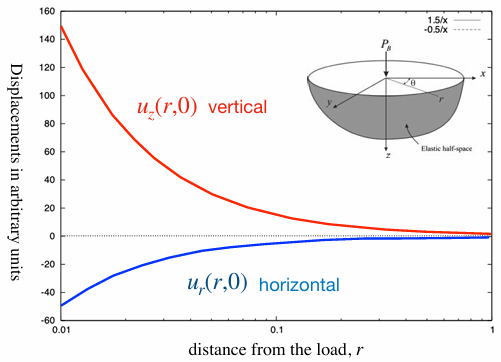
\includegraphics[width=0.5\linewidth]{fig/boussinesq.png}
    \caption{Deformazione orizzontale e verticale dovuta ad un carico nel modello di Boussinesq.}
    \label{fig:boussinesq}
\end{figure}

\noindent
Si calcolano le deformazioni sulla superficie $(z = 0)$ in questo modello compressibile (Figura \ref{fig:boussinesq}).
La componente verticale $u_z$ è sempre positiva, quindi diretta verso il basso: non c'è nessun \textit{forebulge}, ovvero una deformazione verso l'alto.
La deformazione in direzione radiale $u_r$ è negativa, quindi avviene verso il centro.
Per $x \rightarrow 0$ c'è una singolarità.\\

\noindent
Il problema di Kelvin coinvolge un carico puntiforme su corpo elastico infinito;
il problema di Cerruti riguarda invece un carico puntiforme orizzontale sulla superficie di una massa semi-infinita.
Questi due problemi possono essere applicati in geomeccanica per risolvere il problema di Boussinesq.\\

\noindent
I carichi applicabili alla Terra sono di due diversi tipi: superficiale (con contatto) o mareale (che non prevede contatto).
Lo studio delle maree non si può affrontare con il modello di Boussinesq.
Kelvin cercò di determinare la rigidità della Terra grazie alle maree, in seguito Darwin applicò un modello sferico per lo studio delle maree su una sfera fluida.
La soluzione di Kelvin può essere applicata all’isostasia glaciale.

Nel 1972 Farrell introdusse il formalismo delle funzioni di Green per una Terra sferica. 
Discusse l’approssimazione della Terra piatta per deformazioni locali e calcolò i numeri di Love fino al grado $l=10^4$. 
Il modello di Boussinesq diventa il limite della Terra sfericamente simmetrica e stratificata a piccola scala.
Coi modelli di Farrell e di Boussinesq si modella il rimbalzo post-glaciale.

\subsection{\textcolor{colore7}{Topografia, livello marino e distribuzione di acqua e ghiaccio}}

Si può caratterizzare una distribuzione superficiale di massa grazie alle \textbf{funzione oceano},
definita a partire dallo \textbf{spessore del ghiaccio} $I(\gamma, t)$ e dalla \textbf{topografia} $T(\gamma, t)$:

\begin{equation}
    \mathcal{O}(\gamma,t) \equiv \begin{cases}
        1 \text{ } & \text{ se } T + \frac{\rho^i}{\rho^w}I < 0 \\ 0 \text{ } & \text{ se } T + \frac{\rho^i}{\rho^w}I \ge 0 
    \end{cases}
\end{equation}

\noindent
con $\gamma = (\theta, \lambda)$, $\theta$ e $\lambda$ sono colatitudine e latitudine, rispettivamente.
$\rho^i$ e $\rho^w$ sono le densità costanti di acqua e ghiaccio, rispettivamente.\\

\noindent
Data la topografia $T$, si definiscono la \textbf{funzione livello del mare} $B(\gamma, t)$ come:

\begin{equation}
    B(\gamma, t) = - T(\gamma, t)
\end{equation}

\noindent
e la \textbf{funzione continente}:

\begin{equation}
    \mathcal{C}(\gamma, t) = 1 - \mathcal{O}(\gamma, t)
\end{equation}

\noindent
Si hanno cinque possibilità per i valori della funzione oceano, illustrati nella Figura \ref{fig:ocean_function}.

\begin{figure}[h!]
    \centering
    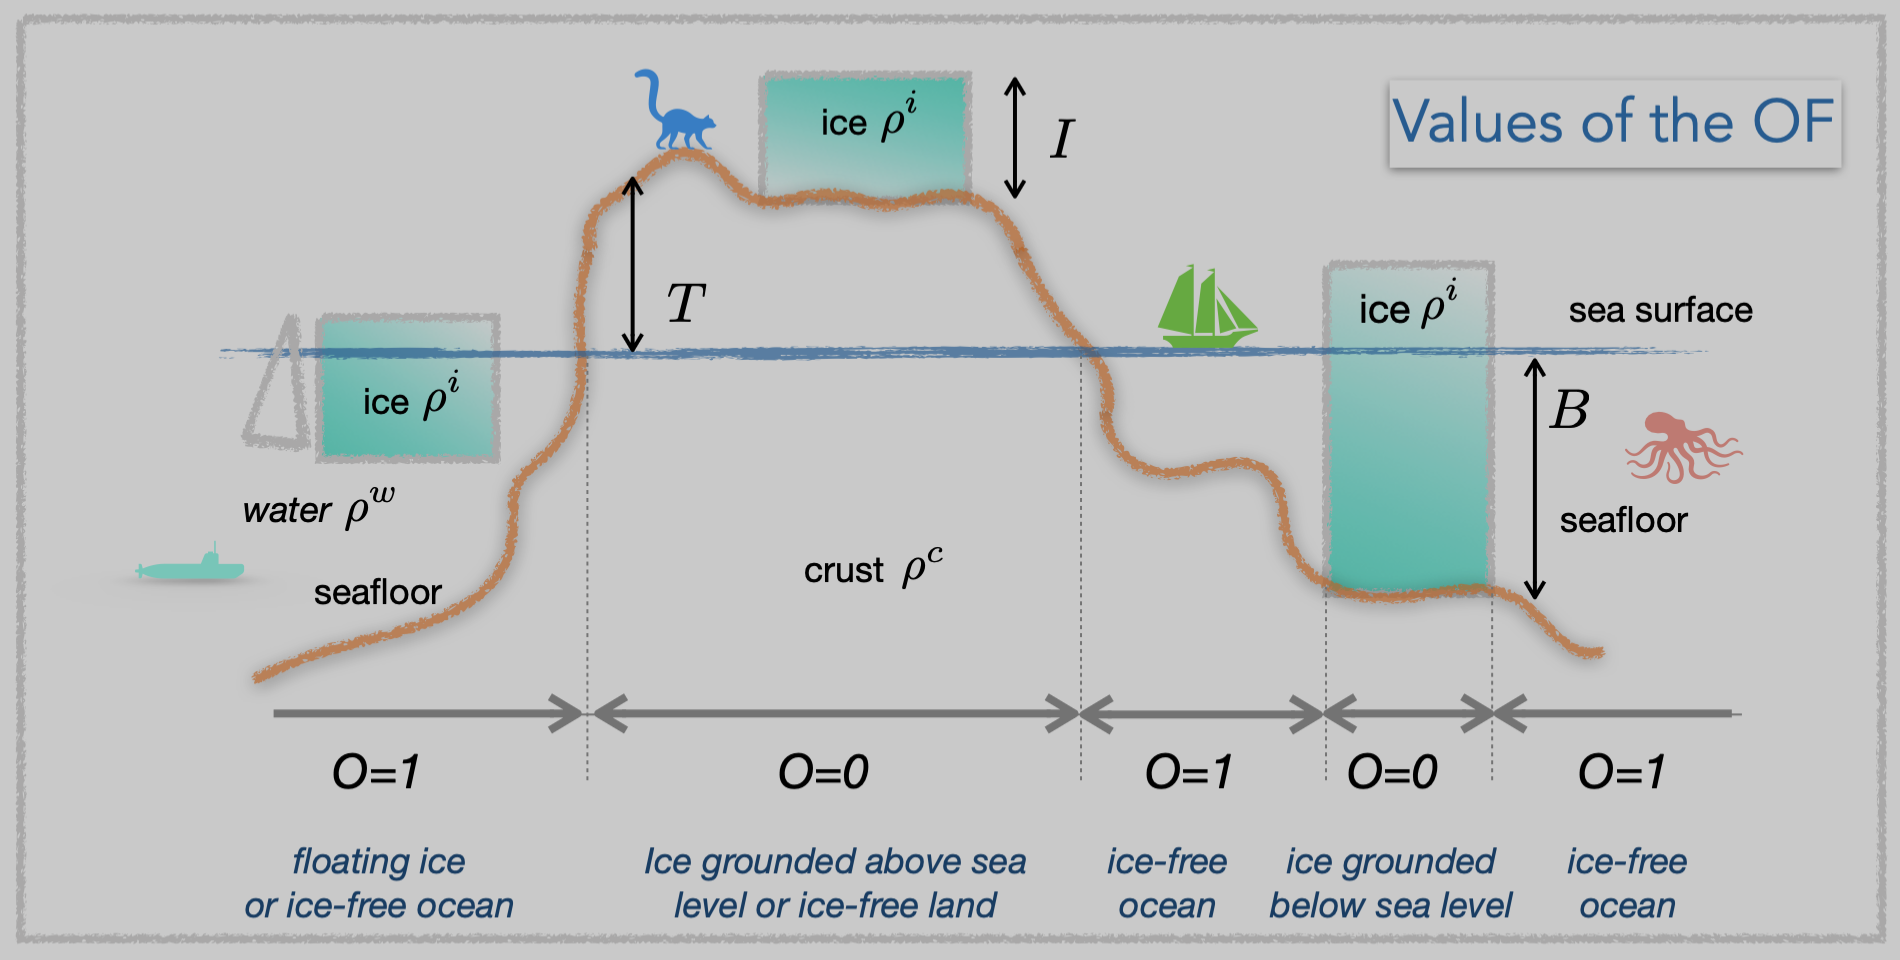
\includegraphics[width=0.5\linewidth]{fig/ocean_function.png}
    \caption{Possibili valori della funzione oceano.}
    \label{fig:ocean_function}
\end{figure}

\noindent
\textbf{Ghiaccio galleggiante} $\mathcal{O} = 1$ ($I>0$ e $T<0$)\\

\noindent
Per principio di isostasia tutte le colonne devono avere la stessa massa: $\rho^w B(\gamma, t) = \rho^i I + \rho^w y$ (Figura \ref{fig:floating_ice}),
con $y$ lo spessore dello strato d'acqua sotto la colonna di ghiaccio.
Dato che $y > 0$, segue che $T(\gamma, t) + \frac{\rho^i}{\rho^w} I(\gamma, t) < 0$, quindi il ghiaccio è più leggero della colonna d'acqua: $\mathcal{O} = 1$ e $\mathcal{C} = 0$.\\

\begin{figure}[h!]
    \centering
    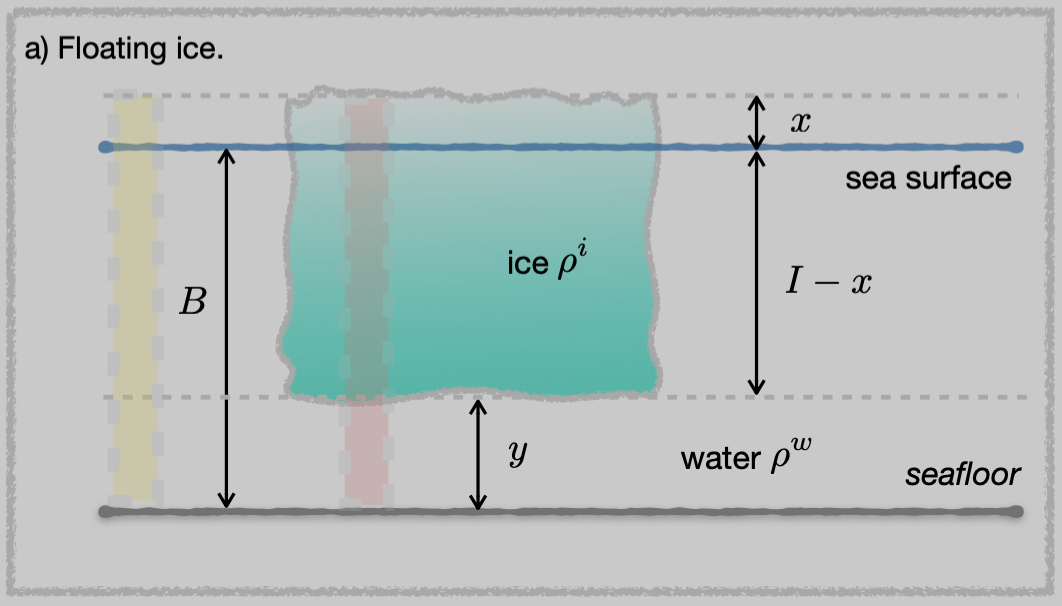
\includegraphics[width=0.5\linewidth]{fig/floating_ice.png}
    \caption{Ghiaccio galleggiante.}
    \label{fig:floating_ice}
\end{figure}

\noindent
\textbf{Ghiaccio che poggia sulla superficie sopra il livello del mare} $\mathcal{O} = 0$ e $\mathcal{C} = 1$ ($I>0$ e $T>0$)\\

\noindent
\textbf{Oceano libero dal ghiaccio} $\mathcal{O} = 1$ ($I=0$ e $T<0$)\\

\noindent
\textbf{Ghiaccio che poggia sulla superficie sotto il livello del mare} $\mathcal{O} = 0$ ($I>0$ e $T<0$)\\

\noindent
Il sistema non è in equilibrio isostatico e le colonne di ghiaccio sono più pesanti delle colonne d'acqua, quindi $T(\gamma, t) + \frac{\rho^i}{\rho^w} I(\gamma, t) \geq 0$.

\begin{figure}[h!]
    \centering
    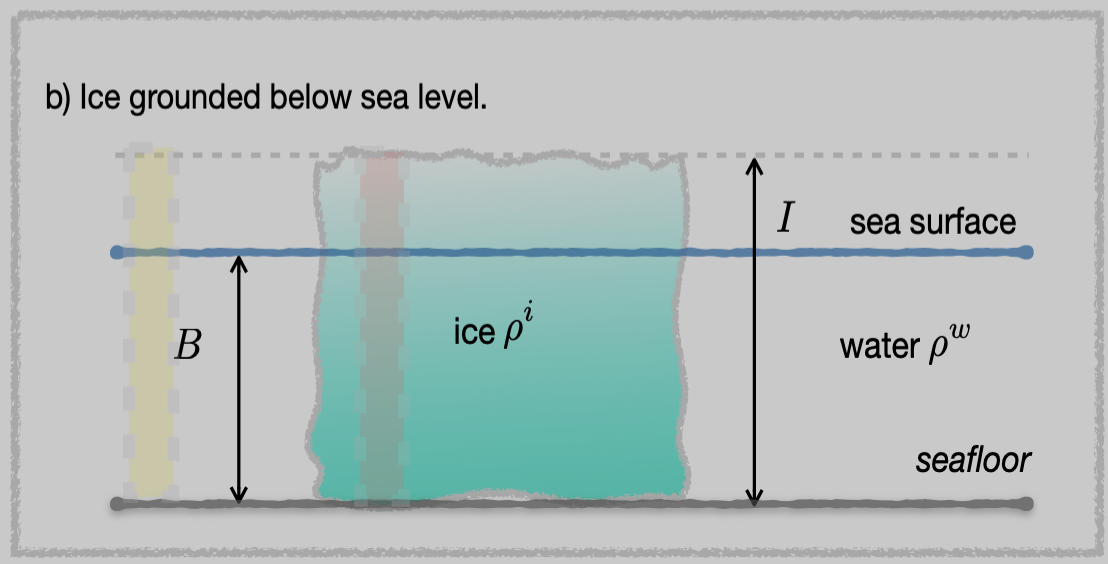
\includegraphics[width=0.5\linewidth]{fig/ice_grounded.png}
    \caption{Ghiaccio che poggia sulla superficie sotto il livello del mare.}
    \label{fig:ice_grounded}
\end{figure}

\noindent
\textbf{Terreno libero dal ghiaccio} $\mathcal{O} = 0$ e $\mathcal{C} = 1$ ($I=0$ e $T>0$)\\

\noindent
Così la funzione oceano determina cosa c'è sotto il ghiaccio.

\begin{figure}[htb]
    \centering
    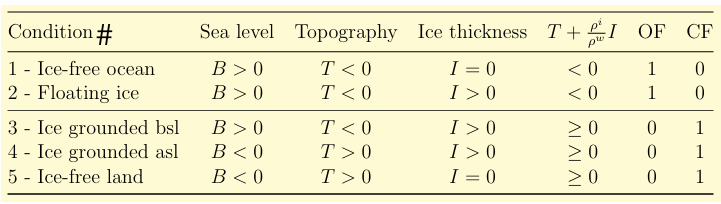
\includegraphics[width=0.7\linewidth]{fig/tabella_oceano.png}
    \caption{Valori della funzione oceano in funzione di topografia, spessore del ghiaccio e casi possibili.}
    \label{fig:tabella_oceano}
\end{figure}

\noindent
Dalla definizione di topografia discende la definizione della \textbf{variazione del livello marino}:

\begin{equation}
    S(\gamma , t) = B - B_0
\end{equation}

\noindent
Dove $B_0 = B(\gamma, t_0)$ è il livello del mare in uno stato di equilibrio di riferimento.
Al tempo presente $t = t_N$ si definisce così $B_N = B(\gamma, t_N)$.

\noindent
La \textbf{variazione della topografia} è data da:

\begin{equation}
    T(\gamma, t) - T(\gamma, t_N) = - (B - B_N) = - [(B - B_0) - (B_N - B_0)]
\end{equation}

\noindent Si definisce allora l'equazione della \textbf{paleotopografia} di Peltier:

\begin{equation}
    T(\gamma, t) = T_N - (\mathcal{S} - \mathcal{S}_N)
\end{equation}

\noindent
Nota la topografia attuale e l’evoluzione del livello marino nel passato, si può così ricostruire la topografia a un istante arbitrario.

Aggiungendo il termine dato dal ghiaccio, si ottiene infine la \textbf{paleotopografia vera}:

\begin{equation}
    PT(\gamma,t) = T + I
\end{equation}

\noindent
Dalla soluzione di questa equazione è stato possibile ricavare i ponti topografici come quello di Doggerland (GBR ed Europa) e Beringia, che hanno favorito gli spostamenti umani.\\

\noindent
Queste funzioni dipendono dallo spazio e dal tempo in maniera continua, ma può essere utile considerare una discretizzazione temporale dei campi e un intervallo costante fra gli istanti successivi.

L’asse temporale viene suddiviso in diversi time step e grazie alla funzione di Heaviside si può ricostruire $F(\gamma , t)$ tramite una somma finita:

\begin{equation}
    F(\gamma, t) = F_0 (\gamma) + \sum_{k=0}^N [F_{k+1}(\gamma) - F_k (\gamma) ] H(t-t_k)
\end{equation}

\noindent
Si ottiene una funzione costante a tratti.
La \textbf{variazione temporale} di $F(\gamma,t)$ è data dalla differenza tra il valore attuale e quello di equilibrio:

\begin{equation}
    \mathcal{F}(\gamma, t) \equiv F(\gamma, t) - F_0 (\gamma)
\end{equation}

\noindent
Anche questa può essere discrettizzata:

\begin{equation}
    \mathcal{F}(\gamma, t) = \sum_{k=0}^N [\mathcal{F}_{k+1}(\gamma) - \mathcal{F}_k (\gamma)] H(t-t_k)
\end{equation}

\subsection{\textcolor{colore7}{Funzione di carico superficiale e sue variazioni temporali}}

Il \textbf{carico superficiale} rappresenta la massa per unità di area, dipendente dalla posizione e dal tempo.
Data la \textbf{massa distribuita sulla superficie terrestre} $M(t)$, la \textbf{funzione il carico superficiale} è descritta da $L(\gamma, t)$:

\begin{equation}
    M(t) = \int_e L (\gamma, t) dA \equiv a^2 \int_0^{2\pi} \int_0^\pi L(\gamma, t) sin \theta d \theta d \lambda \Longrightarrow L(\gamma, t) = \frac{dM}{dA}
\end{equation}

\noindent
dove $a$ è il raggio terrestre. L'integrazione avviene sulla superficie della Terra coperta da acqua o ghiaccio.\\

\noindent
Ad un dato tempo $t$, si possono distinguere i contributi: $M(t) = M^i(t) + M^w (t)$, con $M^i$ e $M^w$ la massa di ghiaccio e d'acqua, rispettivamente.
Distinguiamo ulteriormente il ghiaccio \textit{grounded} (sia sopra che sotto il livello del mare) da quello \textit{floating}:

\begin{equation}
    M^i(t) = M^{i,gr}(t) + M^{i,fl}(t)
\end{equation}

\noindent
Integrando su tutta la Terra filtrando con la funzione continente si trova la massa del ghiaccio:

\begin{equation}
    M^i(t) = \rho^i \int_e ICdA + \rho^i \int_{fl}IdA
\end{equation}

\noindent In maniera analoga si trova quella dell’acqua anche grazie alle regioni con ghiaccio galleggiante.
Il water term si può scrivere anche in funzione di $y$, cioè la distanza tra il ghiaccio galleggiante e il fondale marino:

\begin{equation}
    M^w(t) = M^{w,if} + M^{w,fl} = \rho^w \int_{if}BdA + \rho^i\int_{fl}ydA
\end{equation}

\noindent
dove $if$ indica oceani privi di ghiaccio (\textit{ice-free}) e $fl$ quelli con ghiaccio galleggiante (\textit{floating ice}).
Imponendo la condizione di isostasia sulla variabile $y$ per il ghiaccio galleggiante si ottiene:

\begin{equation}
    M^w(t) = \rho^w \int_{if}BdA + \int_{fl} (\rho^wB - \rho^i I)dA
\end{equation}

\noindent Grazie alle proprietà della funzione oceano si cancellano dei termini che fanno restare:
\begin{equation}
    M(t) = \rho^i \int_e ICdA + \rho^i \int_{fl} IdA + \rho^w \int_{if}BdA + \rho^w \int_{fl}BdA - \rho^i \int_{fl} IdA = \int_e (\rho^i IC + \rho^w BO)dA
\end{equation}

\noindent Si ottiene un'espressione utilissima per il carico superficiale:

\begin{equation}
    L(\gamma , t) = \rho ^i I C + \rho^ w BO
\end{equation}

\noindent
che è estremamente simmetrica.\\

\noindent
Si definisce la \textbf{variazione temporale del carico superficiale}

\begin{equation}
    \mathcal{L}(\gamma,t) = L - L_0 = \rho^i (IC - I_0C_0) + \rho^w(BO-B_0O_0)
\end{equation}

\noindent
Si introducono anche la \textbf{variazione dello spessore del ghiaccio}

\begin{equation}
    \mathcal{I}(\gamma, t) = I - I_0
\end{equation}

\noindent
e la \textbf{variazione della funzione oceano}:

\begin{equation}
    \mathcal{O}(\gamma, t) = O - O_0
\end{equation}

\noindent
Con le definizioni viste fino a qui si ritrova così un’altra equazione molto simmetrica, per la variazione del carico superficiale:

\begin{equation}
    \mathcal{L}(\gamma, t) = \rho^i C\mathcal{I} + \rho^w O\mathcal{S} - (\rho^i I_0 + \rho^w T_0)\mathcal{O}
    \label{eq:variazione_carico}
\end{equation}

\noindent
Inoltre, è possibile suddividere la variazione nei contributi dovuti alla variazione dello spessore del ghiaccio, del livello del mare e della funzione oceano:

\begin{equation}
    \mathcal{L}(\gamma, t) = \mathcal{L}^a + \mathcal{L}^b + \mathcal{L}^c
\end{equation}

\noindent
dove $\mathcal{L}^a (\gamma, t) \equiv \rho^i \mathcal{W}$,
$\mathcal{L}^b (\gamma, t) \equiv \rho^w \mathcal{Z}$,
$\mathcal{L}^c (\gamma, t) \equiv \rho^r \mathcal{X}$.

Con $\mathcal{W} (\gamma, t) \equiv \mathcal{C} \mathcal{I}$,
$\mathcal{Z} (\gamma, t) \equiv \mathcal{O} \mathcal{S}$,
$\mathcal{X} (\gamma, t) \equiv \mathcal{Q} \mathcal{O}$,
associati alle variazioni dello spessore del ghiaccio, del livello del mare e della funione oceano, rispettivamente.

\subsection{\textcolor{colore7}{Conservazione della massa}}

\begin{figure}[h!]
    \centering
    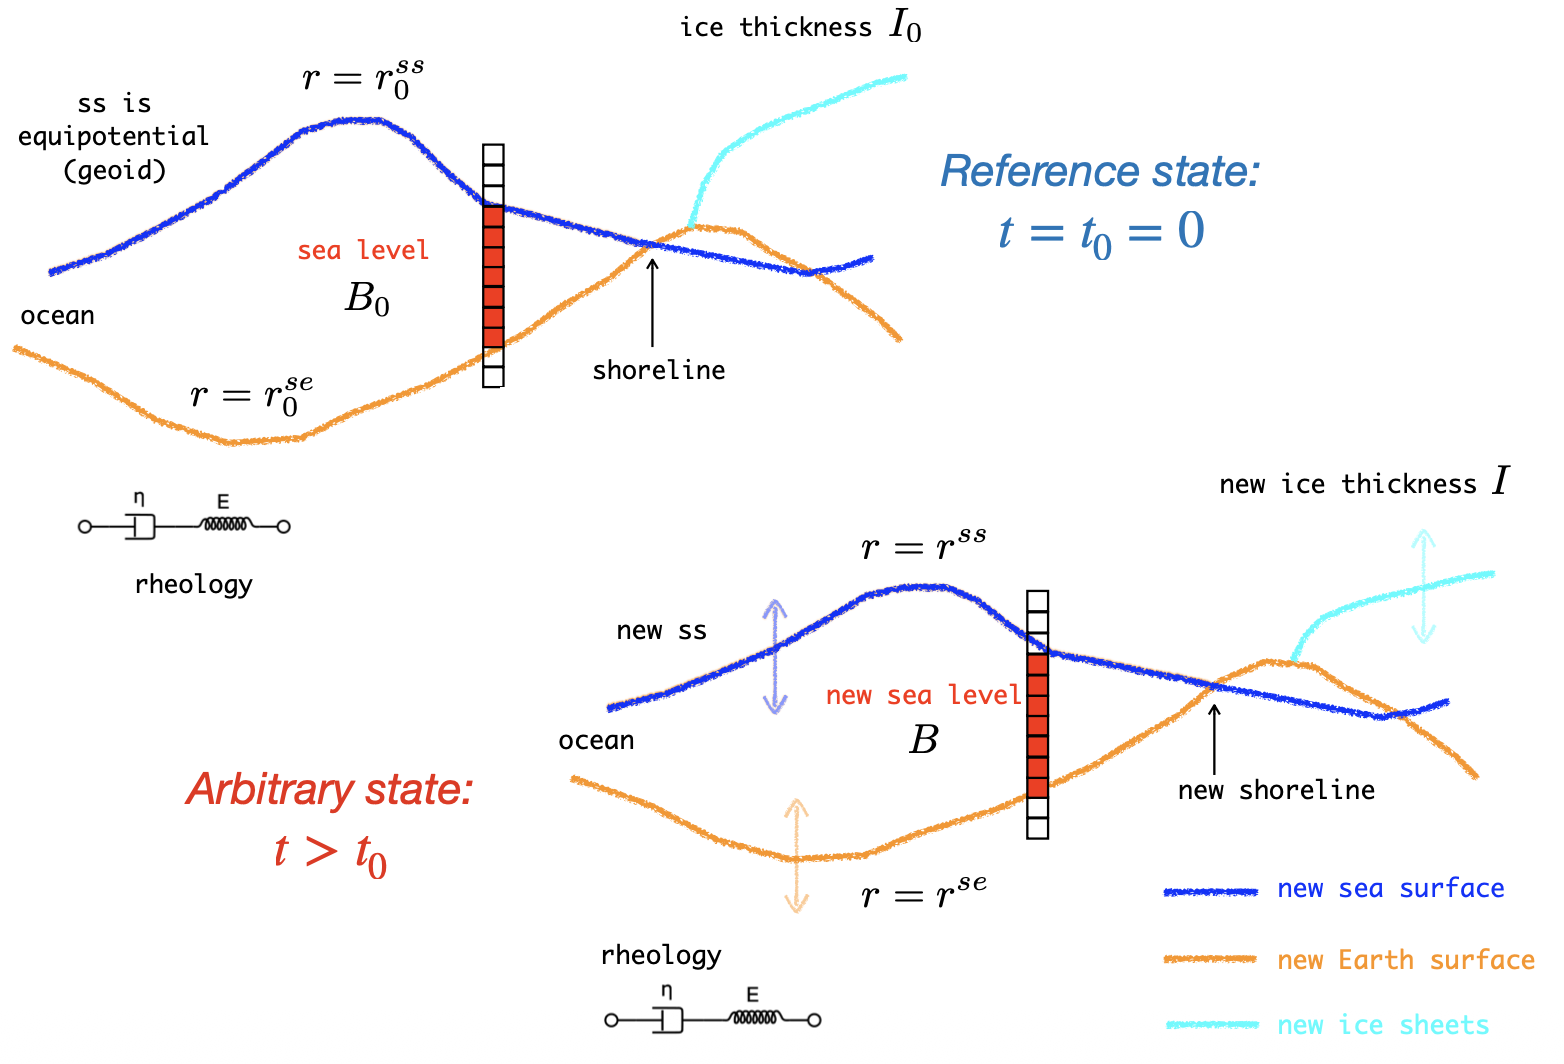
\includegraphics[width=0.6\linewidth]{fig/mass_conservation_01.png}
    \caption{Conservazione della massa.}
\end{figure}

\noindent
Si considerano un istante iniziale $t_0$, in cui si ha equilibrio e la reologia è latente, e uno arbitrario $t$, in cui le funzioni hanno assunto nuovi valori.
Il vincolo fondamentale dell'equazione del livello marino è il \textbf{principio di conservazione della massa}, che si può applicare in diversi modi.
Nella forma base, vale $M(t) = M_0$.
In forma integrale 

\begin{equation}
    \mathcal{M}(t) \equiv M - M_0 \equiv \int_e \mathcal{L}dA = 0
\end{equation}

\noindent
che si può esprimere anche tramite la media della variazione del carico superficiale sulla superficie della Terra:

\begin{equation}
    \langle \mathcal{L}(\gamma, t) \rangle^e \equiv \frac{1}{A^e} \int_e \mathcal{L}(\gamma, t) dA
\end{equation}

\noindent
Con $A^e = \int_e dA = 4\pi a^2$ l'area della superficie terrestre. 
Grazie allo sviluppo in funzioni armoniche, inoltre, vale:

\begin{equation}
    F(\gamma, t) = \sum_{lm} F_{lm} (t) \mathcal{Y}_{lm}(\gamma) \quad \Longrightarrow \quad \langle F(\gamma, t)\rangle = \frac{1}{4\pi} \int_\gamma F(\gamma, t) dA = F_{00}(t)
\end{equation}

\noindent
Con $F_{00}(t)$ è il grado zero armonico nell'espansione in armoniche sferiche in forma complessa.
Perciò la conservazione della massa si può esprimere anche tramite:

\begin{equation}
    \mathcal{L}_{00}(t)=0
\end{equation}

\noindent
Un'altra forma si può ottenere a partire dall'espressione all'eq. \ref{eq:variazione_carico}:

\begin{equation}
    \mathcal{M}(t) \equiv \int_e \mathcal{L}dA = \rho^i \int_e (IC - I_0C_0)dA + \rho^w \int_e (BO-B_0O_0)dA=0
\end{equation}

\noindent Esprimendo ora la \textbf{variazione della massa del ghiaccio grounded} con:

\begin{equation}
    \mu(t) = \rho^i \int_e (IC-I_0C_0)dA
\end{equation}

\noindent Si ottiene un'altra forma del principio di conservazione della massa, relativa al solo ghiaccio grounded:

\begin{equation}
    \mu(t) + \rho^w \int_e (BO-B_0O_0)dA = 0
\end{equation}

\noindent Riscrivendo la differenza:

\begin{align}
    BO-B_0O_0 &= (B-B_0+B_0)O-B_0O_0 \\ &= (B-B_0)O + (B_0(O-O_0) \\ &= \mathcal{S}O + B_0 \mathcal{O} \\ &= \mathcal{S}O - T_0\mathcal{O}
\end{align}

\noindent Così si può riscrivere il principio di conservazione della massa come:

\begin{equation}
    \mu(t) + \rho^w \int_e (BO - B_0O_0)dA = \mu(t) + \rho^w \int_e \mathcal{S}O dA - \rho^w \int_e T_0 \mathcal{O}dA = 0 
\end{equation}

\noindent Da cui si ottiene un'altra forma fondamentale:

\begin{equation}
    \mu(t) + \rho^w A^o <\mathcal{S}>^o - \rho^wA^e <T_0 \mathcal{O}>^e = 0
    \label{eq:MCP3}
\end{equation}

\noindent
dove $<...>^o$ rappresenta la media sull'oceano, che è una superficie variabile nel tempo.\\

\noindent
Per il principio di conservazione della massa, tutta la massa del sistema (acqua + ghaiccio) resta costante.\\

\noindent \textbf{\textcolor{colore7}{Forme del principio di conservazione della massa}}:

\begin{enumerate}
    \item $M(t) = M_0$ o $\mathcal{M}(t) = 0$;
    \item $<\mathcal{L}(\gamma, t)>^e = 0$ o $\mathcal{L}_{00} (t) = 0$;
    \item $\mu(t) + \rho^w \int_e (BO - B_0O_0)dA = 0$ o $\mu(t) + \rho^w A^o <\mathcal{S}>^o - \rho^w A^e<T_0 \mathcal{O}>^e = 0$.
\end{enumerate}

\subsection{\textcolor{colore7}{Numeri di Love e funzioni di Green}}

\subsubsection{\textcolor{colore7}{Modelli sfericamente simmetrici della Terra}}

Nei sistemi a simmetria sferica, come il modello 1D della Terra, si possono applicare questi strumenti.
I modelli 1D sono abbastanza realistici se le discrepanze sono poco rilevanti.
Le assunzioni di base sono:

\begin{enumerate}
    \item Terra isotropa, autogravitante (il campo gravitazionale non cambia) e incomprimibile, quindi si assume che il volume non cambia;
    \item nucleo fluido, uniforme e inviscido;
    \item mantello stratificato sfericamente e con reologia viscoelastica di Maxwell;
    \item litosfera elastica e di spessore uniforme.
\end{enumerate}

\noindent
Questi modelli sono detti 1D perché, data la simmetria sferica, i parametri reologici $\eta$, le costanti di Lame $\lambda$ e $\mu$ e la densità $\rho$ dipendono solo dal raggio $r$.
Tuttavia, dato che il carico superficiale è distribuito in maniera non uniforme, la risposta dei modelli 1D deve essere tridimensionale e dipendente dal tempo.\\

\noindent
Il vantaggio di questi modelli è l'esistenza di soluzioni analitiche ben note.
Ad esempio, per i modelli 1D GIA (Aggiustamento Isostatico Glaciale), la risposta della Terra è ben descritta dai numeri di Love,
per i quali sono disponibili soluzioni a forma chiusa.
A partire da tali assunzioni è poi possibile complicare i modelli includendo la stratificazione e la comprimibilità ed escludendo l'autogravitazione,
usando ad esempio la teoria dei \textit{modi normali viscoelastici}.

\subsubsection{\textcolor{colore7}{Funzione diretta di Green (Terra rigida)}}

Si consideri una massa puntiforme sulla superficie di una Terra rigida e sfericamente simmetrica.
Per effetto della rigidià, lo stress di superficie esercitato dalla massa dovuto al suo stesso peso non causa deformazione.
Il carico, tuttavia, induce una variazione del potenziale gravitazionale della Terra.

\begin{figure}[htb]
    \centering
    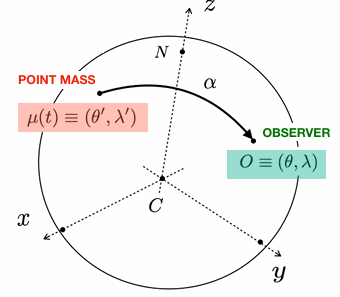
\includegraphics[width=0.3\linewidth]{fig/massa_puntiforme.png}
    \caption{Sistema sorgente osservatore del problema.}
    \label{fig:massa_puntiforme}
\end{figure}

\noindent
La massa puntuale è indicata con una massa effettiva $\mu(t) = \delta(t) \delta m$, dove $\delta m$ è piccolo rispetto alla massa della Terra: $\delta m \ll m_e$.
Il carico superficiale associato è dato da:

\begin{equation}
    \mathcal{L}^\delta (\alpha, t) = \frac{\mu(t)}{a^2} \frac{\delta (\theta - \theta') \delta(\lambda - \lambda')}{sin \theta}
\end{equation}

\noindent
con:

\begin{equation}
    \mathcal{L}^\delta (\alpha, t) dA = \mu(t)
\end{equation}

\noindent La variazione del potenziale gravitazionale presso l'osservatore $O \equiv (\theta, \lambda)$ è detta \textbf{contributo diretto} al potenziale gravitazionale, l'unico nel caso della Terra rigida.

\begin{equation}
    \varphi ^r (\alpha,t) = \frac{G \mu(t)}{d(\alpha)}
\end{equation}

\noindent Dalla trigonometria:

\begin{equation}
    d(\alpha) = 2a sin\left( \frac{a}{2} \right) \Longrightarrow \varphi ^r (\alpha, t) = \delta(t) \frac{ag\delta m}{2m^e sin (\alpha/2)}
\end{equation}

\noindent
dove

\begin{equation}
    g = \frac{G m^e}{a^2}
\end{equation}

\noindent La \textbf{variazione del potenziale per unità di massa e di tempo} è fornita dalla funzione di Green per il potenziale gravitazionale diretto:

\begin{equation}
    \Gamma^{\varphi,r} (\alpha, t) \equiv \frac{\varphi^r (\alpha, t)}{\delta m} = \delta (t) \frac{ag}{m^e} \left( \frac{1}{2sin(\alpha/2)} \right)
\end{equation}

\noindent Siccome la massa è adimensionale, la funzione diverge per $\alpha \longrightarrow 0$, poi decade velocemente con la distanza angolare.
Una forma più utile si ottiene sfruttando i polinomi di Legendre:

\begin{equation}
    \frac{1}{2sin(\alpha/2)} \equiv \sum_{l=0}^\infty P_l (cos \alpha)
\end{equation}

\noindent Si può dare una \textbf{rappresentazione spettrale} della funzione di Green:

\begin{equation}
    \Gamma^{\varphi,r} (\alpha, t) = \delta (t) \sum_{l=0}^\infty \varphi _l^r P_l (cos \alpha)
\end{equation}

\noindent
Dove i coefficienti armonici $\varphi _l^r \equiv \frac{ag}{m^e}$ sono uguali: lo spettro è bianco.

\subsubsection{\textcolor{colore7}{Funzioni di Green incrementali (Terra elastica)}}

Se la Terra è deformabile, la variazione della distribuzione di massa aggiunge un \textbf{contributo indiretto} alla variazione del potenziale gravitazionale,
per cui la funzione di Green corrispondente si può esprimere tramite la seguente espansione:

\begin{equation}
    \Gamma^{\varphi,e} (\alpha, t) \equiv \frac{\varphi ^e (\alpha, t)}{\delta m} = \delta (t) \sum_{l=0}^\infty \varphi_l^e P_l (cos \alpha)
\end{equation}

\noindent Il valore dei coefficienti armonici $\varphi_l^e$ si ricava risolvendo equazioni di equilibrio (mi aspetto che $\varphi_l^e \neq \varphi_l^r$).
Il \textbf{principio di Love} sostiene che tra i coefficienti armonici elastici e quelli relativi alla variazione diretta di potenziale gravitazionale vi sia una relazione diretta:

\begin{equation}
    \varphi_l^e = k_l^{L,e}\varphi_l^r
\end{equation}

\noindent
dove il coefficiente adimensionale $k_l^{L,e} = \varphi_l^e / \varphi_l^r$ è il \textbf{Numero di carico elastico di Love per il potenziale}.
La "$L$" all'apice indica che si riferisce al carico, mentre per le maree si ha una "$T$".
Per una Terra rigida $k_l^{L,e} = 0$, mentre nel caso reale il valore è compreso fra 0 e 1.\\

\noindent La \textbf{funzione di Green per il potenziale totale di una Terra elastica} è:

\begin{equation}
    \Gamma^\varphi (\alpha, t) \equiv \Gamma^{\varphi,r} + \Gamma^{\varphi,e} = \delta(t) \frac{ag}{m^e} \sum_{l=0}^\infty (1 + k_l^{L,e})P_l(cos\alpha)
\end{equation}


\noindent Applicando la formula di Brun (eq. \ref{eq:Brun}), si può ottenere un'espressione per la \textbf{funzione di Green per la variazione dell'altezza del geoide} per unità di massa e di tempo:
\begin{equation}
    \Gamma^g (\alpha, t) \equiv \frac{\Gamma^\varphi}{g} = \delta (t) \frac{a}{m^e} \sum_{l=0}^\infty (1 + k_l^{L,e})P_l(cos \alpha)
\end{equation}

\noindent
Dove nelle parentesi compaiono il termine $1$ che descrive la variazione diretta e il termine $k_l^{L,e}$ che descrive l'effetto indiretto dovuto all'elasticità della Terra.
A causa degli effetti elastici, si ha anche uno spostamento verticale, per cui si esprime anche la \textbf{funzione di Green elastica dello spostamento verticale}:

\begin{equation}
    \Gamma^{u}(\alpha, t) = \delta(t) \frac{a}{m^e} \sum_{l=0}^\infty h_l^{L,e} P_l (cos \alpha)
\end{equation}

\noindent E analogamente la \textbf{funzione di Green elastica dello spostamento orizzontale}: 

\begin{equation}
    \vec{\Gamma}^v (\alpha, t) \equiv \delta(t) \frac{a}{m^e} \sum_{l=0}^\infty l _l^{L,e} \partial_\alpha P_l (cos \alpha) \hat{\alpha}
\end{equation}

\noindent
dove $_l$ e $l_l$ sono i Loading Love Number verticali e orizzontali.\\

\noindent Si hanno così tre funzioni di Green: una per l'altezza del geoide, una per lo spostamento verticale e una per quello orizzontale.
Per una Terra rigida si avrebbe $(h,k,l)_l^{L,e} \equiv 0$, mentre per una elastica i numeri di Love sono del tipo $j_l^L (t) = j_l ^{L,e} \delta (t)$, con $j = h, k ,l$.

\subsubsection{\textcolor{colore7}{Numeri di Love elastici}}

I numeri di Love $(h, k, l)$ sono parametri adimensionali che misurano la suscettibilità della forma di un corpo planetario a un potenziale perturbativo (originariamente mareale).
Introdotti originariamente da Love (1909) per la risposta elastica globale alle maree, il termine può indicare:

\begin{itemize}
    \item Tidal Love numbers: per le deformazioni indotte dalle maree;
    \item Loading Love numbers (LLN): utilizzati per calcolare le funzioni di Green, quindi la risposta della Terra a carichi superficiali;
    \item Dislocation Love numbers: dove la sorgente è interna e impulsiva, come nel caso dei terremoti.
\end{itemize}

\noindent
I numeri di Love dipendono dalle proprietà fisiche della Terra: la geometria del modello sferico, lo spessore, la densità e le costanti elastiche dei vari strati,
dalle condizioni al contorno e dalla lunghezza d'onda del carico.\\

\noindent
A causa di questa complessità, non esiste un'espressione analitica chiusa generale, ma si ricorre a modelli numerici.
Nel lavoro di Farrell (1972), i numeri di Love elastici da carico sono stati calcolati in funzione del grado armonico $n$.\\

\subsubsection{\textcolor{colore7}{Funzioni di Green viscoelastiche}}

Nello studio dei modi normali viscoelastici introdotto da Paltier (1974) si dimostra che la risposta della Terra a un carico impulsivo non è istantanea,
ma presenta un contributo ritardato nel tempo dovuto al riassestamento viscoso del mezzo.\\

\noindent
Per un modello di Terra 1D a simmetria sferica con reologia lineare i numeri di Love da carico sono funzioni causali (nulle per $t < 0$) e caratterizzate da due componenti fisicamente distinte:

\begin{itemize}
    \item Componente elastica: in fase con il carico impulsivo ($\delta$ di Dirac), dipendente esclusivamente dalle costanti elastiche e dalla densità degli strati.
    \item Componente viscosa: ritardata rispetto al carico, sensibile al profilo reologico oltre che ai parametri elastici.
\end{itemize}

\noindent
La componente viscosa assume una forma multiesponenziale determinata dallo spettro dei modi normali viscoelastici.
Quindi, l'espressione per i numeri di Love da carico in funzione del tempo e del grado armonico $l$ è:

\begin{equation}
    k_l^L (t) = k_l^{L,e} \delta (t) + H(t) \sum_{i=1} ^M k_{li}^L e^{s_{li}t}
\end{equation}

\noindent
dove 
\begin{itemize}
    \item $H(t)$ è la funzione gradino di Heaviside che garantisce la causalità della risposta;
    \item $M$ rappresenta il numero di modi viscoelastici, che dipende dal numero di strati;
    \item $k_{li}^L$ è l'ampiezza del termine viscoso associato al $k$-esimo LLN;
    \item $s_{li} = - 1/\tau_{li}<0$ è la matrice di frequenze complesse che descrive il decadimento tramite i tempi scala caratteristici del modello $\tau_{li}$.\\
\end{itemize}

\noindent
I valori dei numeri di Love al grado $l=1$ dipendono dalla scelta del sistema di riferimento;
per convenzione, essi vengono espressi nel sistema centrato al centro di massa (CM) del sistema Terra + Carico.\\

\noindent \textbf{\textcolor{colore7}{Numeri di Love per spostamenti verticali e orizzontali}}

\noindent
Nel formalismo dei modi normali viscoelastici (VNM), indicando con $x(t)$ un generico numero di Love da carico (LLN) associato a una forzante impulsiva $\delta$,
la scomposizione spettrale per un modello di Terra 1D assume la forma generale:

\begin{equation}
    x_l (t) = x_l^{e} \delta (t) + H(t) \sum_{i=1} ^M x_{li}^L e^{s_{li}t}
\end{equation}

\noindent
Per i rispettivi LLN di spostamento verticale ($h_l^L$) e orizzontale ($\ell_l^L$), le espressioni nel dominio del tempo sono:

\begin{equation}
    h_l^L (t) = h_l^{L,e} \delta (t) + H(t) \sum_{i=1} ^M h_{li}^L e^{s_{li}t}
\end{equation}

\begin{equation}
    l_l^L (t) = l_l^{L,e} \delta (t) + H(t) \sum_{i=1} ^M l_{li}^L e^{s_{li}t}
\end{equation}

\noindent
dove $0 \le l \le \infty$ e $i = 1,..., M$.
Le funzioni di Green hanno la stessa forma del caso elastico, ma i numeri di Love hanno anche una parte ritardata.\\

\noindent \textbf{\textcolor{colore7}{Numeri di Love di Heaviside}}

\noindent
Se il sistema è soggetto ad un carico costante nel tempo applicato istantaneamente a $t=0$, la sorgente viene modellata tramite la funzione di Heaviside $H(t)$.
Il corrispondente numero di Love di Heaviside $x^H(t)$ si ricava per convoluzione dal coefficiente impulsivo:

\begin{equation}
    x^H(t) \equiv x(t) * H(t) \equiv x_e - \sum_i \frac{x_i}{s_i} (1-e^{s_i t})
\end{equation}

\noindent
Il \textbf{limite elastico} $(t\longrightarrow 0)$ descrive la risposta elastica istantanea del mezzo al momento dell'applicazione del carico:

\begin{equation}
    \lim_{t \longrightarrow 0} x^H(t) = x_e
\end{equation}

\noindent
Il \textbf{limite fluido} $(t\longrightarrow \infty)$ descrive lo stato asintotico a lungo periodo in cui le tensioni viscose si sono completamente rilassate e il mezzo raggiunge l'equilibrio:

\begin{equation}
    \lim_{t \longrightarrow \infty} x^H(t) = x_f = x_e - \sum_i \frac{x_i}{s_i}
\end{equation}

\noindent
Nei casi intermedi si hanno transizioni complesse che vengono considerate per processi come l'isostasia glaciale.\\

\subsection{\textcolor{colore7}{Calcolo dei numeri di Love}}

\subsubsection{\textcolor{colore7}{Equazioni di equilibrio}}

Il calcolo dei numeri di Love richiede una stima degli spostamenti e delle variazioni del potenziale gravitazionale di una Terra 1-dimensionale,
soggetta ad un carico superficiale unitario.
Le equazioni di equilibrio con le opportune condizioni di regolarità e al contorno da risolvere sono:

\begin{enumerate}
    \item Conservazione del momento in un continuo: $\nabla \cdot \sigma + \rho \vec{g} = 0$;
    \item Equazione di Laplace per il potenziale gravitazionale: $\nabla^2 \varphi = 0$;
    \item Conservazione della massa tramite equazione di continuità: $\nabla \cdot \vec{u} = 0$;
    \item Equazione costitutiva, data dalla legge di Hooke: $\sigma = \sigma (\varepsilon, \dot{\varepsilon}, ..., \vec{p})$.
\end{enumerate}

\noindent
Si sfrutta la simmetria del problema per separare la parte angolare da quella radiale, dal quale si ottiene un sistema di equazioni differenziali ordinarie del I ordine, che si risolve nel dominio di Laplace con il metodo dei propagatori.

\subsubsection{\textcolor{colore7}{Modello di Kelvin e altri modelli analitici}}

Il modello di Kelvin (KM) rappresenta un caso di fondamentale importanza nella geodinamica globale grazie alla sua semplicità analitica e un sufficiente grado di realismo:
viene infatti considerato un "modello di Terra medio".
Esso consiste in una sfera omogenea, elastica (o viscoelastica) e incompressibile, definita univocamente da tre soli parametri indipendenti:
il raggio $a$, la densità $\rho$ e la rigidità $\mu$.
L'accelerazione di gravità alla superficie per questo modello è espressa da $g = \frac{4}{3}\pi G \rho a$.
Nel caso viscoelastico (VE KM), il modello viene caratterizzato aggiungendo un opportuno numero di parametri reologici (es. viscosità).\\

\noindent
Per il modello di Kelvin puramente elastico, è possibile ricavare le espressioni analitiche esplicite per i numeri di Love di carico per ogni grado armonico $l \ge 2$:

\begin{equation}
    k_l^{L,e} = -\frac{1}{1 + \lambda_l \xi}, \quad h_l^{L,e} = -\frac{(2l + 1)/3}{1 + \lambda_l \xi}, \quad \ell_l^{L,e} = -\frac{1/l}{1 + \lambda_l \xi}
\end{equation}

\noindent
dove $\lambda_l = \frac{2l^2 + 4l + 3}{l}$ è una costante geometrico-armonica e $\xi = \frac{\mu}{\rho g a}$ rappresenta un parametro adimensionale che pesa il rapporto tra le forze elastiche (rigidità) e quelle gravitazionali.
Per i gradi elastici più bassi, il caso $l=0$ assume LLN nulli per motivi di conservazione della massa del carico superficiale, mentre il caso $l=1$ dipende strettamente dalla scelta del sistema di riferimento.\\

\noindent
Applicando il "Principio di Corrispondenza" della viscoelasticità lineare, è possibile determinare la risposta viscoelastica sostituendo formalmente il modulo di rigidità elastico $\mu$ con il modulo complesso $\tilde{\mu}(s)$.
Ad esempio, adottando una reologia Maxwelliana, la sostituzione assume la forma:

\begin{equation}
    \mu \longmapsto \tilde{\mu}(s) = \frac{\mu s}{s + 1/\tau}
\end{equation}

\noindent
dove $\tau$ è il tempo di rilassamento di Maxwell.
Sostituendo $\tilde{\mu}(s)$ nelle espressioni dei numeri di Love si ottiene la risposta nel dominio delle frequenze, la quale, per frequenze che tendono a zero ($s \to 0$) o per rigidità che svanisce ($\tilde{\mu} \to 0$),
converge ai cosiddetti \textit{fluid limits}:

\begin{equation}
    k_n^{L,f} = -1, \quad h_n^{L,f} = -\frac{2n+1}{3}, \quad \ell_n^{L,f} = -\frac{1}{n}
\end{equation}

\noindent
Nel caso elastico di Kelvin i numeri di Love sono monoesponenziali, mentre nei casi con un maggior numero di strati si ha una dipendenza da esponenziali multipli.

Forme analitiche dei numeri di Love sono disponibili anche per modelli a 2 strati, ma sono complesse e rendono più comodo l'uso di approcci numerici.

\subsubsection{\textcolor{colore7}{Approcci numerici ai numeri di Love}}

Partendo da un semplice modello con una litosfera elastica, un mantello a tre strati e un nucleo fluido omogeneo, si scopre che i numeri di Love trovati da diversi codici numerici differiscono fra loro.
Le sfere stratificate hanno molti tempi scala caratteristici che dipendono dal grado armonico considerato.

\newpage

\section{\textcolor{colore7}{Surface loading ed equazione del livello marino II}}

\subsection{\textcolor{colore7}{Risposta a carichi superficiali finiti}}

\subsubsection{\textcolor{colore2}{Motivazione}}

Si passa dalla schematizzazione ideale di carichi puntiformi e impulsivi allo studio di problemi di carico reali,
caratterizzati da distribuzioni di massa estese e variabili sia nello spazio che nel tempo.

I carichi reali non sono statici né localizzati in un singolo punto; essi comprendono tutte le masse instabili presenti al di sopra della superficie terrestre, tra cui l'atmosfera, l'idrosfera, la criosfera e le strutture vulcaniche.

\subsubsection{\textcolor{colore2}{Surface response functions (SRF)}}

Si considerano carichi distribuiti nello spazio che evolvono nel tempo.
A partire dalle soluzioni delle equazioni di equilibrio per una sfera stratificata si ricavano i numeri di Love.
Da un'opportuna combinazione lineare di essi si ricavano le funzioni di Green.
Si accoppiano le funzioni di Green con un carico superficiale grazie a una convoluzione tridimensionale per ottenere le \textbf{Surface response function} (\textbf{SRF}).
In seguito, si fa conduce un'analisi spettrale.
Si può arrivare alle SRF a partire dalla soluzione dell'equazione del livello marino o da un'assunzione di carico uniforme.

\begin{figure}[h!]
    \centering
    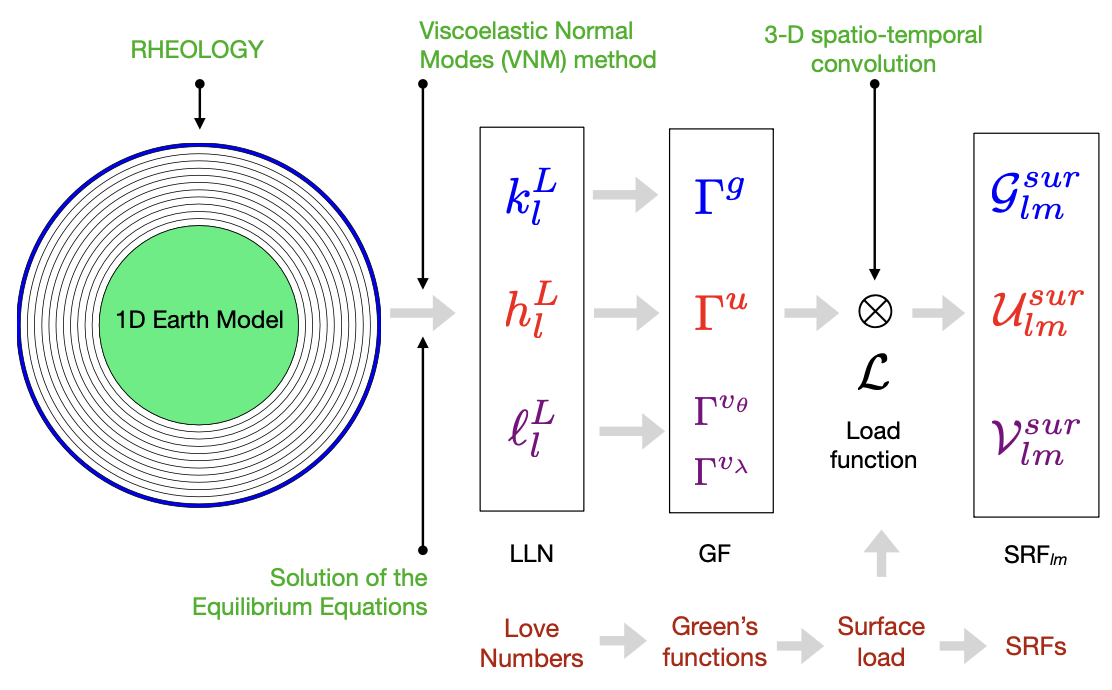
\includegraphics[width=0.7\linewidth]{fig/SRF.png}
    \caption{Flusso per determianre le SRF.}
\end{figure}

\noindent
Una SRF rappresenta la risposta della Terra ad una variazione di un carico finito nello spazio e nel tempo:

\begin{equation}
    \mathcal{L} = \mathcal{L}(\gamma, t)
\end{equation}

\noindent
Permette di conoscere la variazione dell'altezza del geoide ($\mathcal{G}(\gamma, t)$), lo spostamento orizzontale ($\mathcal{V}_\theta (\gamma,t)$ e $\mathcal{V}_\lambda (\gamma,t)$) e verticale ($\mathcal{U}(\gamma,t)$) e la variazione del livello marino ($\mathcal{R} (\gamma, t) = \mathcal{G} - \mathcal{U}$).

\subsubsection{\textcolor{colore7}{Convoluzione tridimensionale}}

Le SRF hanno forma generale:

\begin{equation}
    SRF(\gamma,t) = (\Gamma \otimes \mathcal{L} )
\end{equation}

\noindent
dove $\Gamma = \Gamma (\gamma, t)$ è una funzione di Green e $\mathcal{L} = \mathcal{L}(\gamma, t)$ è una funzione di carico.
La convoluzione tridimensionale (data da due dimensioni spaziali e una temporale) è quindi:

\begin{equation}
    SRF(\gamma,t) = (\Gamma \otimes \mathcal{L} ) (\gamma,t) \equiv \int_{-\infty}^{+\infty} dt' \int_e \Gamma (\alpha, t-t') \mathcal{L}(\gamma', t') dA'
\end{equation}

\noindent
$\Gamma (\gamma,t)$ dipende solo dai numeri di Love e dalle proprietà del modello, con gli effetti diretti e indiretti,
mentre $\mathcal{L} (\gamma,t)$ dipende dalla geometria e dall'evoluzione spaziale e temporale del carico, come per esempio quello di ghiaccio e acqua.

\subsubsection{\textcolor{colore7}{Forma spettrale delle SRF}}

Si espande la funzione di carico superficiale in armoniche sferiche:

\begin{equation}
    \mathcal{L}(\gamma,t) = \sum_{lm} \mathcal{L}_{lm}(t) \mathcal{Y}_{lm} (\gamma)
\end{equation}

\noindent
con coefficienti:

\begin{equation}
   \mathcal{L}_{lm}(t) = \frac{1}{4\pi} \int_\gamma \mathcal{L}(\gamma,t) \mathcal{Y}_{lm}^* (\gamma) d\gamma
\end{equation}

\noindent
Si riscrive la forma generale della funzione di Green:

\begin{equation}
    \Gamma (\alpha, t) = \frac{a}{m^e} \sum_{l=0}^\infty x_l (t) P_l (cos \alpha)
\end{equation}

\noindent
dove $x_l$ rappresenta una combinazione di numeri di Love che dipende dalla SRF:

\begin{equation}
x_l(t) \equiv 
\left\{
\begin{aligned}
  \delta(t) + k_l^L(t), &\quad \mapsto \Gamma = \Gamma^g &\quad \mapsto SRF = \mathcal{G}; \\
  h_l^L(t),              &\quad \mapsto \Gamma = \Gamma^u &\quad \mapsto SRF = \mathcal{U}; \\
  \delta(t) + k_l^L(t) - h_l^L(t), &\quad \mapsto \Gamma = \Gamma^g - \Gamma^u &\quad \mapsto SRF = \mathcal{R};
\end{aligned}
\right.
\end{equation}

\noindent La SRF dipende dai numeri di Love e dai coefficienti spettrali $\mathcal{L}_{lm}$ del carico superficiale complessivo $\mathcal{L}(\gamma,t)$, che dipende da tre termini distinti:

\begin{equation}
    \mathcal{L}(\gamma,t) = \rho^i C \mathcal{I} + \rho^w O \mathcal{S} - (\rho^i I_0 + \rho^w T_0) \mathcal{O}
\end{equation}

\noindent
dove:
\begin{itemize}
    \item $\mathcal{I}$: variazioni del carico di ghiaccio;
    \item $\mathcal{S}$: variazioni del livello del mare;
    \item $\mathcal{O}$: variazioni della funzione oceano.
\end{itemize}

\noindent
Mentre il carico glaciale può essere assunto come "noto" (input del modello),
le variazioni del livello del mare e della funzione oceano sono incognite interdipendenti.
Esse non possono essere conosciute a priori senza prima aver risolto la \textbf{Sea Level Equation (SLE)}, ovvero l'equazione fondamentale del GIA.\\

\noindent
Di conseguenza, come primo passo, si adotta un \textbf{approccio semplificato al problema del carico superficiale}, introducendo tre assunzioni:

\begin{itemize}
    \item il ghiaccio è "dato" (noto);
    \item la variazione del livello del mare è nota e uniforme;
    \item la funzione oceano ($\mathcal{O}$) è costante.
\end{itemize}

\subsubsection{\textcolor{colore7}{Approccio semplificato al carico superficiale}}

Mentre la Sea Level Equation (SLE) rappresenta l'equazione fondamentale per l'Aggiustamento Isostatico Glaciale (GIA), il suo utilizzo richiede un approccio gravitazionalmente coerente risolvibile solo per via numerica e iterativa. Per tale motivo, risulta utile introdurre un \textbf{problema di carico semplificato} che ammette una \textbf{soluzione analitica in forma chiusa} senza necessità di iterazioni. 
Sebbene questo approccio trascuri l'autogravitazione e presenti limitazioni, esso consente di determinare l'ordine di grandezza delle variabili coinvolte nel GIA, di modellare in modo molto realistico il Rimbalzo Post-Glaciale (PGR).\\

\noindent
Nel modello si assume che la distribuzione di massa superficiale $\sigma^{iw}(\gamma,t)$ sia una combinazione lineare del carico del ghiaccio ($\sigma^i$) e del carico dell'acqua di fusione ($\sigma^w$):

\begin{equation}
    \sigma^{iw}(\gamma,t) = \sigma^i (\gamma,t) + \sigma^w (\gamma,t) = \rho^i d^i(\gamma) \chi^i(\gamma) f^i(t) + \rho^w d^w(t) \chi^w(\gamma)
\end{equation}

\noindent
Dove:
\begin{itemize}
    \item $\rho^i, \rho^w$ sono le densità di ghiaccio e acqua;
    \item $d^i(\gamma)$ è lo spessore (noto) del ghiaccio nella posizione $\gamma$, mentre $f^i(t)$ ne modula la storia temporale;
    \item $\chi^i(\gamma)$ e $\chi^w(\gamma)$ sono le funzioni maschera (0 o 1) definite su domini spaziali disgiunti (ipotesi di assenza di ghiaccio marino e shorelines fisse);
    \item $d^w(t)$ è lo spessore dello strato di meltwater, assunto \textbf{spazialmente uniforme} sulla superficie oceanica (ipotesi eustatica).
\end{itemize}

\noindent
L'andamento temporale dello spessore del livello del mare $d^w(t)$, inizialmente incognito, viene ricavato imponendo il \textbf{Principio di Conservazione della Massa} (MCP), il quale richiede che la media globale del carico sulla superficie terrestre sia nulla:

\begin{equation}
    \langle \sigma^{iw}(\gamma,t) \rangle^e = 0
\end{equation}

\noindent
Da questa condizione si ottiene analiticamente lo spessore del livello del mare:

\begin{equation}
    d^w(t) = -\frac{\rho^i}{\rho^w} \frac{\langle d^i(\gamma)\chi^i(\gamma) \rangle^e}{\langle \chi^w(\gamma) \rangle^e} f^i(t)
\end{equation}

\noindent
dove il segno meno indica che un aumento dello spessore glaciale è compensato da un abbassamento uniforme del livello del mare (e viceversa).\\

\noindent
Generalizzazione ad \textbf{elementi multipli}:
Il problema si generalizza  al caso di $n^i$ elementi glaciali disgiunti e non sovrapposti all'oceano:

\begin{equation}
    \sigma^{iw}(\gamma,t) = \rho^i \sum_{n=1}^{n^i} \left( d^{i,n}(\gamma) \chi^{i,n}(\gamma) f^{i,n}(t) \right) + \rho^w d^w(t) \chi^w(\gamma)
\end{equation}

\noindent
Generalizzazione ad \textbf{geometrie specifiche}:
Il problema è risolvibile analiticamente per carichi superficiali assialsimmetrici attorno all'asse $z$.
In particolare, se lo spessore $h$ è costante si parla di \textit{Mascon}, ma si possono considerare anche casi in cui lo spessore varia con l'angolo colatitudinale, ovvero $d^i = d^i(\theta)$.\\

\subsubsection{\textcolor{colore7}{Carichi discoidali, carichi di calotte e altri carichi}}

Nel caso di un carico dato da un disco, è possibile utilizzare il modello per descrivere carichi dalla geometria più complessa (anche se con sovrapposizioni e interstizi).
Siccome la litosfera funge da filtro passa-basso, questo problema non costituisce una limitazione.

Nel caso, più realistico, di ghiacciai con il profilo parabolico, tipico delle lenzuola glaciali, si ottiene un paraboloide sulla superficie di una sfera, che ha una descrizione analitica data dai polinomi di Legendre grazie ai \textit{polinomi di Chebyshev} $T_n(\alpha) = cos (n \alpha)$.

Con dei carichi rettangolari si evita il problema di sovrapposizione e interstizi, ma sono meno realistici.
In ogni caso si può imporre la conservazione della massa su tutto il globo o solo su aree specifiche.

\subsubsection{\textcolor{colore7}{Esempio di codice basato sul modello di Peltier}}

Con \textbf{TABOO} si può simulare un ghiacciaio che si assottiglia senza ritirarsi, distinguendo tre fasi: equilibrio isostatico iniziale con spessore costante, fase di deglaciazione (assunta lineare), rimbalzo post-glaciale.
Così si osserva che sotto a un ghiacciaio di circa 2000 metri di spessore si ha una depressione della litosfera di circa 500 metri (in accordo con le densità relative di ghiaccio e mantello); inoltre, si osserva anche un innalzamento laterale al bordo del carico.
TABOO permette anche di calcolare i numeri di Love, ma non di risolvere l'equazione del livello marino.

\subsection{\textcolor{colore7}{Introduzione all'equazione del livello marino}}

Si tratta di un'equazione integrale o implicita, per cui esistono diverse forme di complessità crescente.
Tiene in considerazione la reologia, la variazione dei ghiacci e del livello del mare (definito come la distanza tra la superficie della Terra solida e la superficie del mare).\\

\noindent
\textbf{\textcolor{colore7}{Forma base}}\\

\begin{figure}[h!]
    \centering
    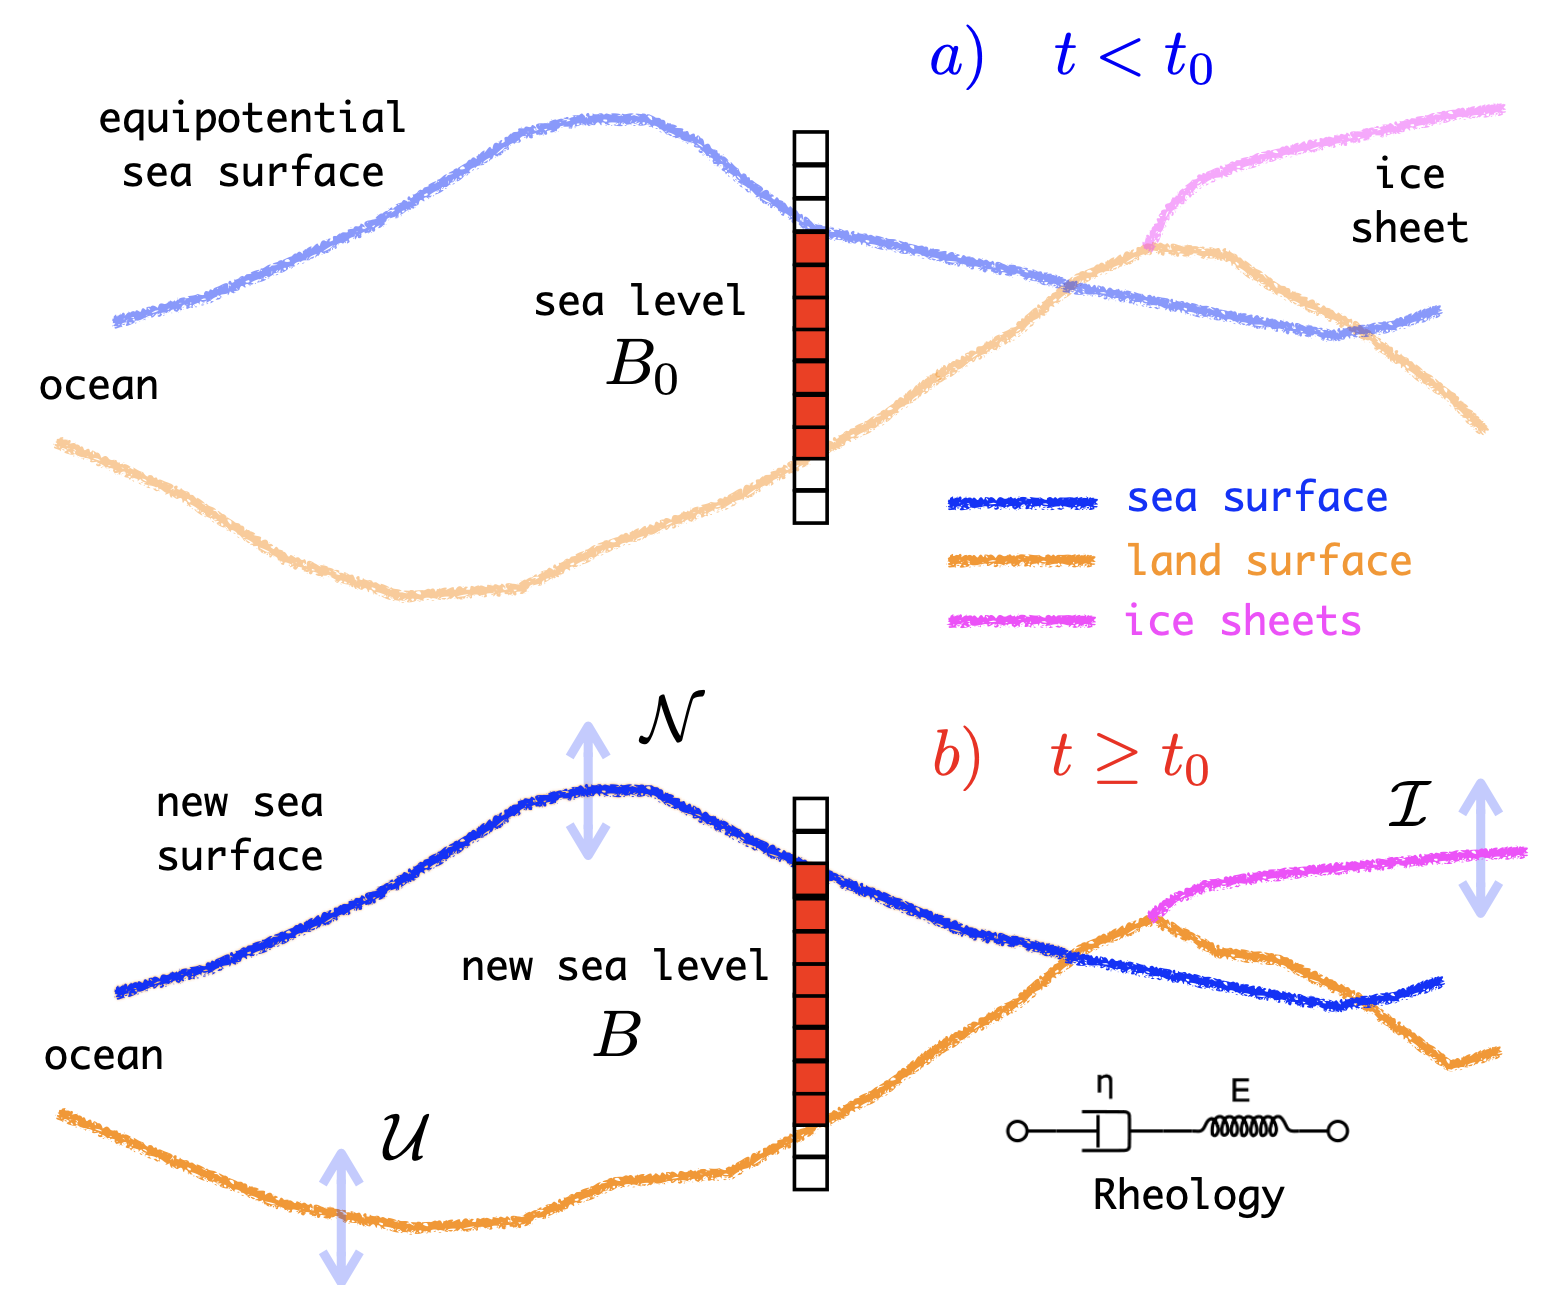
\includegraphics[width=0.5\linewidth]{fig/mass_conservation_02.png}
    \caption{Conservazione della massa.}
    \label{fig:mass_cons}
\end{figure}

\noindent
Al tempo $t$ e in $\gamma$, il livello del mare può essere definito come l'offset tra la superficie del mare e la superficie solida della Terra.
Di conseguenza, per stabilire una forma base per la SLE, confrontiamo i due stati del sistema (Terra Solida + Criosfera + Oceani) mostrati in Figura \ref{fig:mass_cons}, quindi
uno stato di riferimento iniziale ed uno a un tempo arbitrario:

\begin{equation}
    B_0 (\gamma) = r_0^{ss} - r_0^{se}
\end{equation}

\begin{equation}
    B(\gamma, t) = r^{ss} - r^{se}
\end{equation}

\noindent
dove $ss$ si riferisce alla superficie del mare e $se$ a quella della Terra solida.\\

\noindent
La \textbf{variazione del livello marino relativo} è data dalla differenza:

\begin{equation}
    \mathcal{S}(\gamma, t) = B(\gamma, t) - B_0 (\gamma) = (r^{ss} - r_0^{ss}) - (r^{se} - r_0^{se})
\end{equation}

\noindent
La \textbf{variazione del livello marino assoluto} è dato da:

\begin{equation}
    \mathcal{N}(\gamma, t) = r^{ss} - r_0^{ss}
\end{equation}

\noindent
Lo \textbf{spostamento verticale della superficie della Terra solida} è data da:

\begin{equation}
    \mathcal{U}(\gamma, t) = r^{se} - r_0^{se}
\end{equation}

\noindent
Si ricava così la \textbf{forma base dell'equazione del livello marino}:

\begin{equation}
    \mathcal{S}(\gamma, t) = \mathcal{N} - \mathcal{U}
\end{equation}

\noindent
che fornisce la variazione della superficie del mare rispetto al fondale, come viene misurata da un mareografo.\\

\noindent
$\mathcal{N}$ è legato alla variazione dell'altezza del geoide, ma differisce perché la massa dell'oceano cambia a causa della variazione della massa glaciale.
La variazione dell'altezza del geoide è fornita dalla formula di Brun:

\begin{equation}
    \mathcal{G}(\gamma,t) = \frac{\Phi}{g}
\end{equation}

\noindent
dove $\Phi$ è la variazione del potenziale di gravità totale del Sistema Terra.
Si definisce così una costante non trascurabile (varia di circa $0.2 \div 0.3$ mm/anno) $c$ da cui:

\begin{equation}
    \mathcal{N} = \mathcal{G} + c
\end{equation}

\noindent Mettendo insieme queste informazioni, si ricava la \textbf{prima forma dell'equazione del livello marino}:

\begin{equation}
    \mathcal{S}(\gamma, t) = \mathcal{G} - \mathcal{U} + c
\end{equation}

\noindent Per passare a forme più complesse, si considera la media sull'oceano:

\begin{equation}
    <\mathcal{S}>^o (t) = <\mathcal{G} - \mathcal{U}>^o + <c>^o
\end{equation}

\noindent
dove $<F>^o \equiv \frac{1}{A^o} \int_o F(\gamma, t) dA$.\\

\noindent Siccome $c$ è costante nello spazio, si ricava così:

\begin{equation}
    c(t) = <\mathcal{S}>^o - <\mathcal{G} - \mathcal{U}>^o
\end{equation}

\noindent Si ottiene così la \textbf{seconda forma dell'equazione del livello marino}:

\begin{equation}
    \mathcal{S}(\gamma, t) = (\mathcal{G} - \mathcal{U}) + \mathcal{S}^{ave} - <\mathcal{G} - \mathcal{U}>^o
\end{equation}

\noindent
dove $\mathcal{S}^{ave} \equiv <\mathcal{S}>^o$.\\

\noindent
Applicando la terza forma del principio di conservazione della massa (eq. \ref{eq:MCP3}), si ottiene:

\begin{equation}
    \mathcal{S}^{ave} (t) = \mathcal{S}^{equ} + \mathcal{S}^{ofu} \equiv - \frac{\mu}{\rho^w A^o} + \frac{A^e}{A^o} <T_0 \mathcal{O}>^e
\end{equation}

\noindent
dove $\mathcal{S}^{equ}$ è la variazione del livello marino equivalente (non eustatico) e $\mathcal{S}^{ofu}$ è il termine associato alla variazione della funzione oceano.
Queste due quantità sono così dinamiche, dipendendo dal tempo e dalla reologia, a differenza del livello eustatico.\\

\noindent
La variazione dell'altezza del geoide $\mathcal{G}(\gamma, t)$ e lo spostamento verticale $\mathcal{U}(\gamma, t)$ dipendono da un carico superficiale (\textit{sur}) e dalla deformazione rotazionale (\textit{rot}):

\begin{equation}
    \mathcal{G}(\gamma, t) = \mathcal{G}^{sur} + \mathcal{G}^{rot} , \quad \mathcal{U}(\gamma, t) = \mathcal{U}^{sur} + \mathcal{U}^{rot}
\end{equation}

\noindent Si introduce la \textbf{funzione di risposta totale del livello marino}:

\begin{equation}
    \mathcal{R}(\gamma,t) = \mathcal{G} - \mathcal{U} = \mathcal{R}^{sur} + \mathcal{R}^{rot}
\end{equation}

\noindent
con $\mathcal{R}^{sur} (\gamma, t) = \mathcal{G}^{sur} - \mathcal{U}^{sur}$ e con $\mathcal{R}^{rot} (\gamma, t) = \mathcal{G}^{rot} - \mathcal{U}^{rot}$.\\

\noindent Si ottiene così la \textbf{terza forma dell'equazione del livello marino}:

\begin{equation}
    \mathcal{S}(\gamma,t) = \mathcal{R} + \mathcal{S}^{ave} - \langle R \rangle^0 = (\mathcal{R}^{sur} - \langle \mathcal{R}^{sur} \rangle^o ) + \mathcal{S}^{ave} + (\mathcal{R}^{rot} - \langle\mathcal{R}^{rot} \rangle^o)
\end{equation}

\subsubsection{\textcolor{colore7}{Forma pseudo-spettrale dell'equazione del livello marino}}

L'equazione del livello marino può essere scritta in forma pseudo-spettrale,
particolarmente adatta per la discretizzazione spaziale e temporale e per soluzioni numeriche.
La funzione di risposta totale del livello del mare si ottiene tramite una convoluzione tridimensionale:

\begin{equation}
    \mathcal{R}^{sur}(\gamma,t) = \Gamma^{s} \otimes \mathcal{L}
\end{equation}

\noindent
quindi, tramite decomposizione della variazione del carico superficiale $\mathcal{L} (\gamma, t) = \mathcal{L}^a + \mathcal{L}^b + \mathcal{L}^c$,
si decompone anche $\mathcal{R}^{sur} (\gamma, t) = \mathcal{R}^a + \mathcal{R}^b + \mathcal{R}^c$.\\

\noindent
Si definisce la variabile: $\mathcal{Z}(\gamma,t) = O \mathcal{S}$, si ottiene così la \textbf{forma pseudospettrale dell'equazione del livello marino}:

\begin{equation}
    \mathcal{Z}(\gamma,t) = \mathcal{K}^a + \mathcal{K}^b (\mathcal{Z}) + \mathcal{K}^c + \mathcal{Z}^{ave} + \mathcal{K}^{rot} (\mathcal{Z})
\end{equation}

\noindent L'equazione del livello marino può essere espansa in serie di armoniche sferiche,
tuttavia, dato che la sua soluzione si ottiene numericamente su una griglia sferica, l'approccio pseudo-spettrale è più appropriato di quello spettrale.

\subsubsection{\textcolor{colore7}{Equazione del livello marino di Farrell e Clark}}

L'equazione del livello marino (SLE, \textit{Sea Level Equation}) nella sua formulazione classica è stata introdotta nel lavoro fondamentale di Farrell e Clark (1976 - FC76).\\

\noindent
Nella teoria classica di FC76 vengono fatte tre assunzioni semplificative, rimosse successivamente nella teoria generale della SLE:

\begin{enumerate}
    \item Si trascurano gli effetti della \textbf{rotazione terrestre} sul livello marino.
    \item Si assume che le coste abbiano un \textbf{profilo verticale} (tipo scogliera) coincidente con i confini attuali tra oceani e masse continentali. Come descritto dagli stessi autori, la topografia e la batimetria irregolare vengono ignorate, a meno di non voler considerare la variazione del dominio di integrazione introducendo una funzione oceanica ($OF$) variabile nel tempo.
    \item Si trascura il ghiaccio marino \textbf{grounded}.
\end{enumerate}

L'equazione proposta da FC76 è un'equazione implicita ($\mathcal{S}$ compare sia a destra sia a sinistra del segno di uguale):

\begin{equation}
    \mathcal{S}(\gamma,t) = \rho^i \Gamma^s \otimes_i \mathcal{I} + \rho^w \Gamma^s \otimes_o \mathcal{S} + \mathcal{S}^{eus} - \rho^i < \Gamma^s \otimes_i \mathcal{I}>^o - \rho^w <\Gamma^s \otimes_o \mathcal{S}>^o
\end{equation}

\noindent
Dove:
\begin{itemize}
    \item $\otimes_i$ e $\otimes_o$ rappresentano le convoluzioni spazio-temporali eseguite, rispettivamente, sulle regioni coperte dai ghiacciai e sull'oceano;
    \item $\Gamma^s$ è la Green's function per il carico superficiale;
    \item $\mathcal{I}$ è la variazione dello spessore del ghiaccio e $\mathcal{S}$ è la variazione del livello marino;
    \item $\langle \dots \rangle^o$ indica l'operatore di media spaziale sulla superficie degli oceani;
    \item $\mathcal{S}^{eus}(t)$ è il \textbf{termine eustatico}, definito come:
    \begin{equation}
        \mathcal{S}^{eus}(t) = - \frac{\mu(t)}{\rho^w A^{op}}
    \end{equation}
    dove $A^{op}$ è l'area attuale (costante) degli oceani e $\mu$ è la variazione della massa del ghiaccio.
\end{itemize}

\subsubsection{\textcolor{colore7}{Natura dell'equazione del livello marino}}

L'incognita $\mathcal{S}$ compare sia a destra che a sinistra, anche all'interno di convoluzioni integrali,
per cui si tratta di un'\textit{equazione di Fredholm inomogenea del II tipo}, che ha la forma:

\begin{equation}
    u(x) = f(x) + \int_a^b K(x,x')u(x') dx'
\end{equation}

\noindent Si inizia così da una \textit{reasonable guess}, cioè assumendo $u = u^{(0)}(x)$, poi si reitera ottenendo varie approssimazioni fino a una soglia prestabilita.

\subsection{\textcolor{colore7}{Soluzione dell'equazione del livello marino}}

\subsubsection{\textcolor{colore7}{Soluzione eustatica}}

Omettendo nell'equazione FC76 tutti i termini in cui compaiono le funzioni di Green, si ottiene la \textbf{soluzione eustatica}:

\begin{equation}
    \mathcal{S}(\gamma,t) = \mathcal{S}^{eus}(t) \equiv - \frac{\mu}{\rho^w A^{op}}
\end{equation}

\noindent
Una condizione sufficiente affinché si verifichi questa soluzione è che le funzioni di spostamento verticale ($\mathcal{U}$) e di perturbazione del potenziale gravitazionale ($\mathcal{G}$) siano nulle ($\mathcal{U}=0$, $\mathcal{G}=0$).
Ciò equivale ad assumere:
\begin{enumerate}
    \item Una \textbf{Terra perfettamente rigida} (trascurando la reologia terrestre).
    \item Una \textbf{Terra non gravitante} (assumendo la costante di Newton $G=0$), per cui la ridistribuzione di massa sulla superficie non ne perturba il potenziale gravitazionale.
\end{enumerate}

\noindent
Sotto queste ipotesi, poiché la superficie della Terra non si deforma ($\mathcal{U}=0$), il livello marino relativo ($\mathcal{S}$) coincide esattamente con la variazione assoluta della superficie marina ($\mathcal{N}$), ovvero $\mathcal{S} = \mathcal{N}$. Non vi è quindi alcuna differenza tra variazione del livello marino assoluto e relativo.\\

\noindent
Sebbene la soluzione eustatica sia una pessima approssimazione della realtà, esiste una relazione formale tra quest'ultima e la soluzione effettiva della SLE.
Calcolando la media oceanica $\langle \dots \rangle^o$ di entrambi i membri della SLE di FC76 si ottiene:

\begin{equation}
    \langle \mathcal{S}(\gamma,t) \rangle^o = \mathcal{S}^{eus}(t)
\end{equation}

\noindent
Fisicamente, questo significa che \textbf{la media oceanica della soluzione non eustatica (dinamica) corrisponde esattamente alla soluzione eustatica}.
Questa uguaglianza è una diretta conseguenza della conservazione della massa ed è pertanto indipendente dalla cronologia dei ghiacciai, dalla reologia del mantello, dalla geometria delle coste e dagli effetti rotazionali.

\subsubsection{\textcolor{colore7}{Soluzione di Woodward}}

Per comprendere l'effetto dell'autogravitazione terrestre senza le complicazioni della reologia,
si fa riferimento al modello idealizzato di Woodward.\\

\noindent
Assumendo una \textbf{Terra rigida ed elastica, coperta da un oceano uniforme}, si studia l'effetto dell'istantaneo scioglimento o accumulo di una massa di ghiaccio puntiforme.
A causa dell'attrazione gravitazionale tra la massa d'acqua oceanica e la massa glaciale concentrata:
\begin{itemize}
    \item Il livello del mare \textbf{aumenta} nelle vicinanze della massa glaciale, poiché l'attrazione gravitazionale del ghiaccio "attira" l'acqua verso di sé;
    \item Il livello del mare \textbf{diminuisce} a grande distanza angolare dalla massa di ghiaccio.
\end{itemize}

\noindent
Il livello marino reale corrisponde al valore eustatico medio \textbf{solamente a una distanza angolare critica di circa $20^\circ$} dalla massa perturbatrice. A distanze inferiori l'effetto gravitazionale locale sovrasta il valore medio eustatico, mentre a distanze superiori il livello scende al di sotto di esso.

\subsubsection{\textcolor{colore7}{Forma completa dell'equazione del livello marino}}

\begin{equation}
    S = \frac{\rho_i}{\gamma} G_s \otimes_iI + \frac{\rho_w}{\gamma} G_s \otimes_o S - \frac{m_i}{\rho_w A_o} - \frac{\rho_i}{\gamma} \overline{G_s \otimes_iI} - \frac{\rho_w}{\gamma} \overline{G_s \otimes_oS}
\end{equation}

\noindent
dove:

\begin{itemize}
    \item $S$ è la variazione del livello del mare;
    \item $\rho_i, \rho_w$ sono le densità di ghiaccio e acqua;
    \item $G_s$ è la funzione di Green del livello del mare;
    \item $I$ è la variazione dello spessore del ghiaccio;
    \item $m_i$ è la variazione della massa del ghiaccio;
    \item $A_o$ è l'area degli oceani;
    \item $\otimes_i, \otimes_o$ sono le convoluzioni;
    \item $\overline{(...)}$ è la media sull'oceano.
\end{itemize}

\end{document}